% REMEMBER TO SET LANGUAGE!
\documentclass[a4paper,10pt,english]{article}
\usepackage[a4paper,top=2cm,bottom=2.5cm,left=2.7cm,right=2.7cm,marginparwidth=1.75cm]{geometry}
\usepackage[utf8]{inputenc}
\usepackage[english]{babel}
% Standard stuff
\usepackage{amsmath,graphicx,varioref,verbatim,amsfonts,geometry}
\usepackage{wasysym}
\usepackage{enumitem}
\usepackage{bm}
\newcommand{\uveci}{{\bm{\hat{\textnormal{\bfseries\i}}}}}
\newcommand{\uvecj}{{\bm{\hat{\textnormal{\bfseries\j}}}}}
\DeclareRobustCommand{\uvec}[1]{{%
  \ifcsname uvec#1\endcsname
     \csname uvec#1\endcsname
   \else
    \bm{\hat{\mathbf{#1}}}%
   \fi
}}
% colors in text
\usepackage[usenames,dvipsnames,svgnames,table]{xcolor}
% Hyper refs
\usepackage[colorlinks]{hyperref}
\usepackage{float}
\usepackage{wrapfig}  % For text-wrapping around figures
\usepackage{subcaption}
\usepackage{changepage}

% Document formatting
\setlength{\parindent}{0mm}
\setlength{\parskip}{1.5mm}

%Color scheme for listings
\usepackage{textcomp}
\definecolor{listinggray}{gray}{0.9}
\definecolor{lbcolor}{rgb}{0.9,0.9,0.9}

%Listings configuration
\usepackage{listings}
%Hvis du bruker noe annet enn python, endre det her for å få riktig highlighting.
\lstset{
	backgroundcolor=\color{lbcolor},
	tabsize=4,
	rulecolor=,
	language=python,
        basicstyle=\scriptsize,
        upquote=true,
        aboveskip={1.5\baselineskip},
        columns=fixed,
	numbers=left,
        showstringspaces=false,
        extendedchars=true,
        breaklines=true,
        prebreak = \raisebox{0ex}[0ex][0ex]{\ensuremath{\hookleftarrow}},
        frame=single,
        showtabs=false,
        showspaces=false,
        showstringspaces=false,
        identifierstyle=\ttfamily,
        keywordstyle=\color[rgb]{0,0,1},
        commentstyle=\color[rgb]{0.133,0.545,0.133},
        stringstyle=\color[rgb]{0.627,0.126,0.941}
        }

\newcounter{subproject}
\renewcommand{\thesubproject}{\alph{subproject}}
\newenvironment{subproj}{
\begin{description}
\item[\refstepcounter{subproject}(\thesubproject)]
}{\end{description}}

%Lettering instead of numbering in different layers
%\renewcommand{\labelenumi}{\alph{enumi}}
%\renewcommand{\thesubsection}{\alph{subsection}}

%opening
\title{GEO2320 Oceanography - Cruise Report}
\author{Alessio Canclini}

\begin{document}
\maketitle

\section{Introduction}
Physical Oceanography requires a great deal of observational data due to the complexity of the geophysical system. Certain relations such as the oceanic equation of state, lack a fully physical description and are based on empirical results. When it comes to the momentum equations on the other hand, these are known, but can only be solved approximately due to the high non-linearity. This is done numerically by discretizing the continuous derivatives in the equations resulting in difference equations. The accuracy of computations, when used for prediction, will always be limited by temporal and spatial resolution, which both come at a great computational cost. The discretization, time steps and gird size as well as input data all come with some error.

Thus, ocean observations are extremely important for several reasons. It is what we feed into the models, so the accuracy of the measurements is extremely important for the validity of any prediction. Furthermore, we need observational data to verify fore- and hind casting results from a model. Lastly, since both the models and observations come with their individual uncertainties, a combination of the two often gives the best result. This data assimilation is in essence a weighted sum of the observational and modeled results. The weights being adjusted based on which result is most reliable.

On the 28.09.2023 hydrographic measurements where taken on the University of Oslo's F/F Trygve Braarud research vessel. The vessel covered a hydrographic section starting at the Lysakerelva outlet then sailing towards Bunnefjorden. Students taking GEO2320 at UiO where split into two groups for two separate cruises throughout the day. Similar sections were covered in the morning (starting 6:15z) and afternoon (starting 10:15z). The three main objectives on this cruise where
\begin{enumerate}[label=(\roman*)]
        \item Taking hydrographic (CTD) measurements at several locations
        along the section, some of which were taken both morning and afternoon.
        \item Taking weather and air-sea flux
        measurements at these same locations.
       \item Deploying and tracking drifters with drogues at
        various depths to provide qualitative information about the drift currents and upper ocean velocity shear.
        \item Taking Secchi depth measurements at each location
\end{enumerate}
These methods will be presented more thoroughly in section \ref*{sec:methods} followed by a presentation of the results in section \ref*{sec:results}. In addition to the mentioned in-situ measurements, this section will include ocean circulation model results for the same time and positions. Finally, these results will be discussed in section \ref*{sec:discussion}.% followed by some concluding remarcs in section \ref*{sec:conclusion}.

\section{Data and methods}\label{sec:methods}
All data analysis and plotting was done in Python using the Pandas and Matplotlib libraries. The scripts can be found in two notebooks \href{https://github.com/Alessimc/geo2320_oceanography/blob/main/cruise/hydrographic_plots.ipynb}{here} and \href{https://github.com/Alessimc/geo2320_oceanography/blob/main/cruise/combinedplots.ipynb}{here}. These, although functional, are unfortunately not very readable.

% map
\setlength{\intextsep}{-30pt}
\begin{wrapfigure}{r}{0.45\textwidth}  % Adjust the width as needed
        \centering
        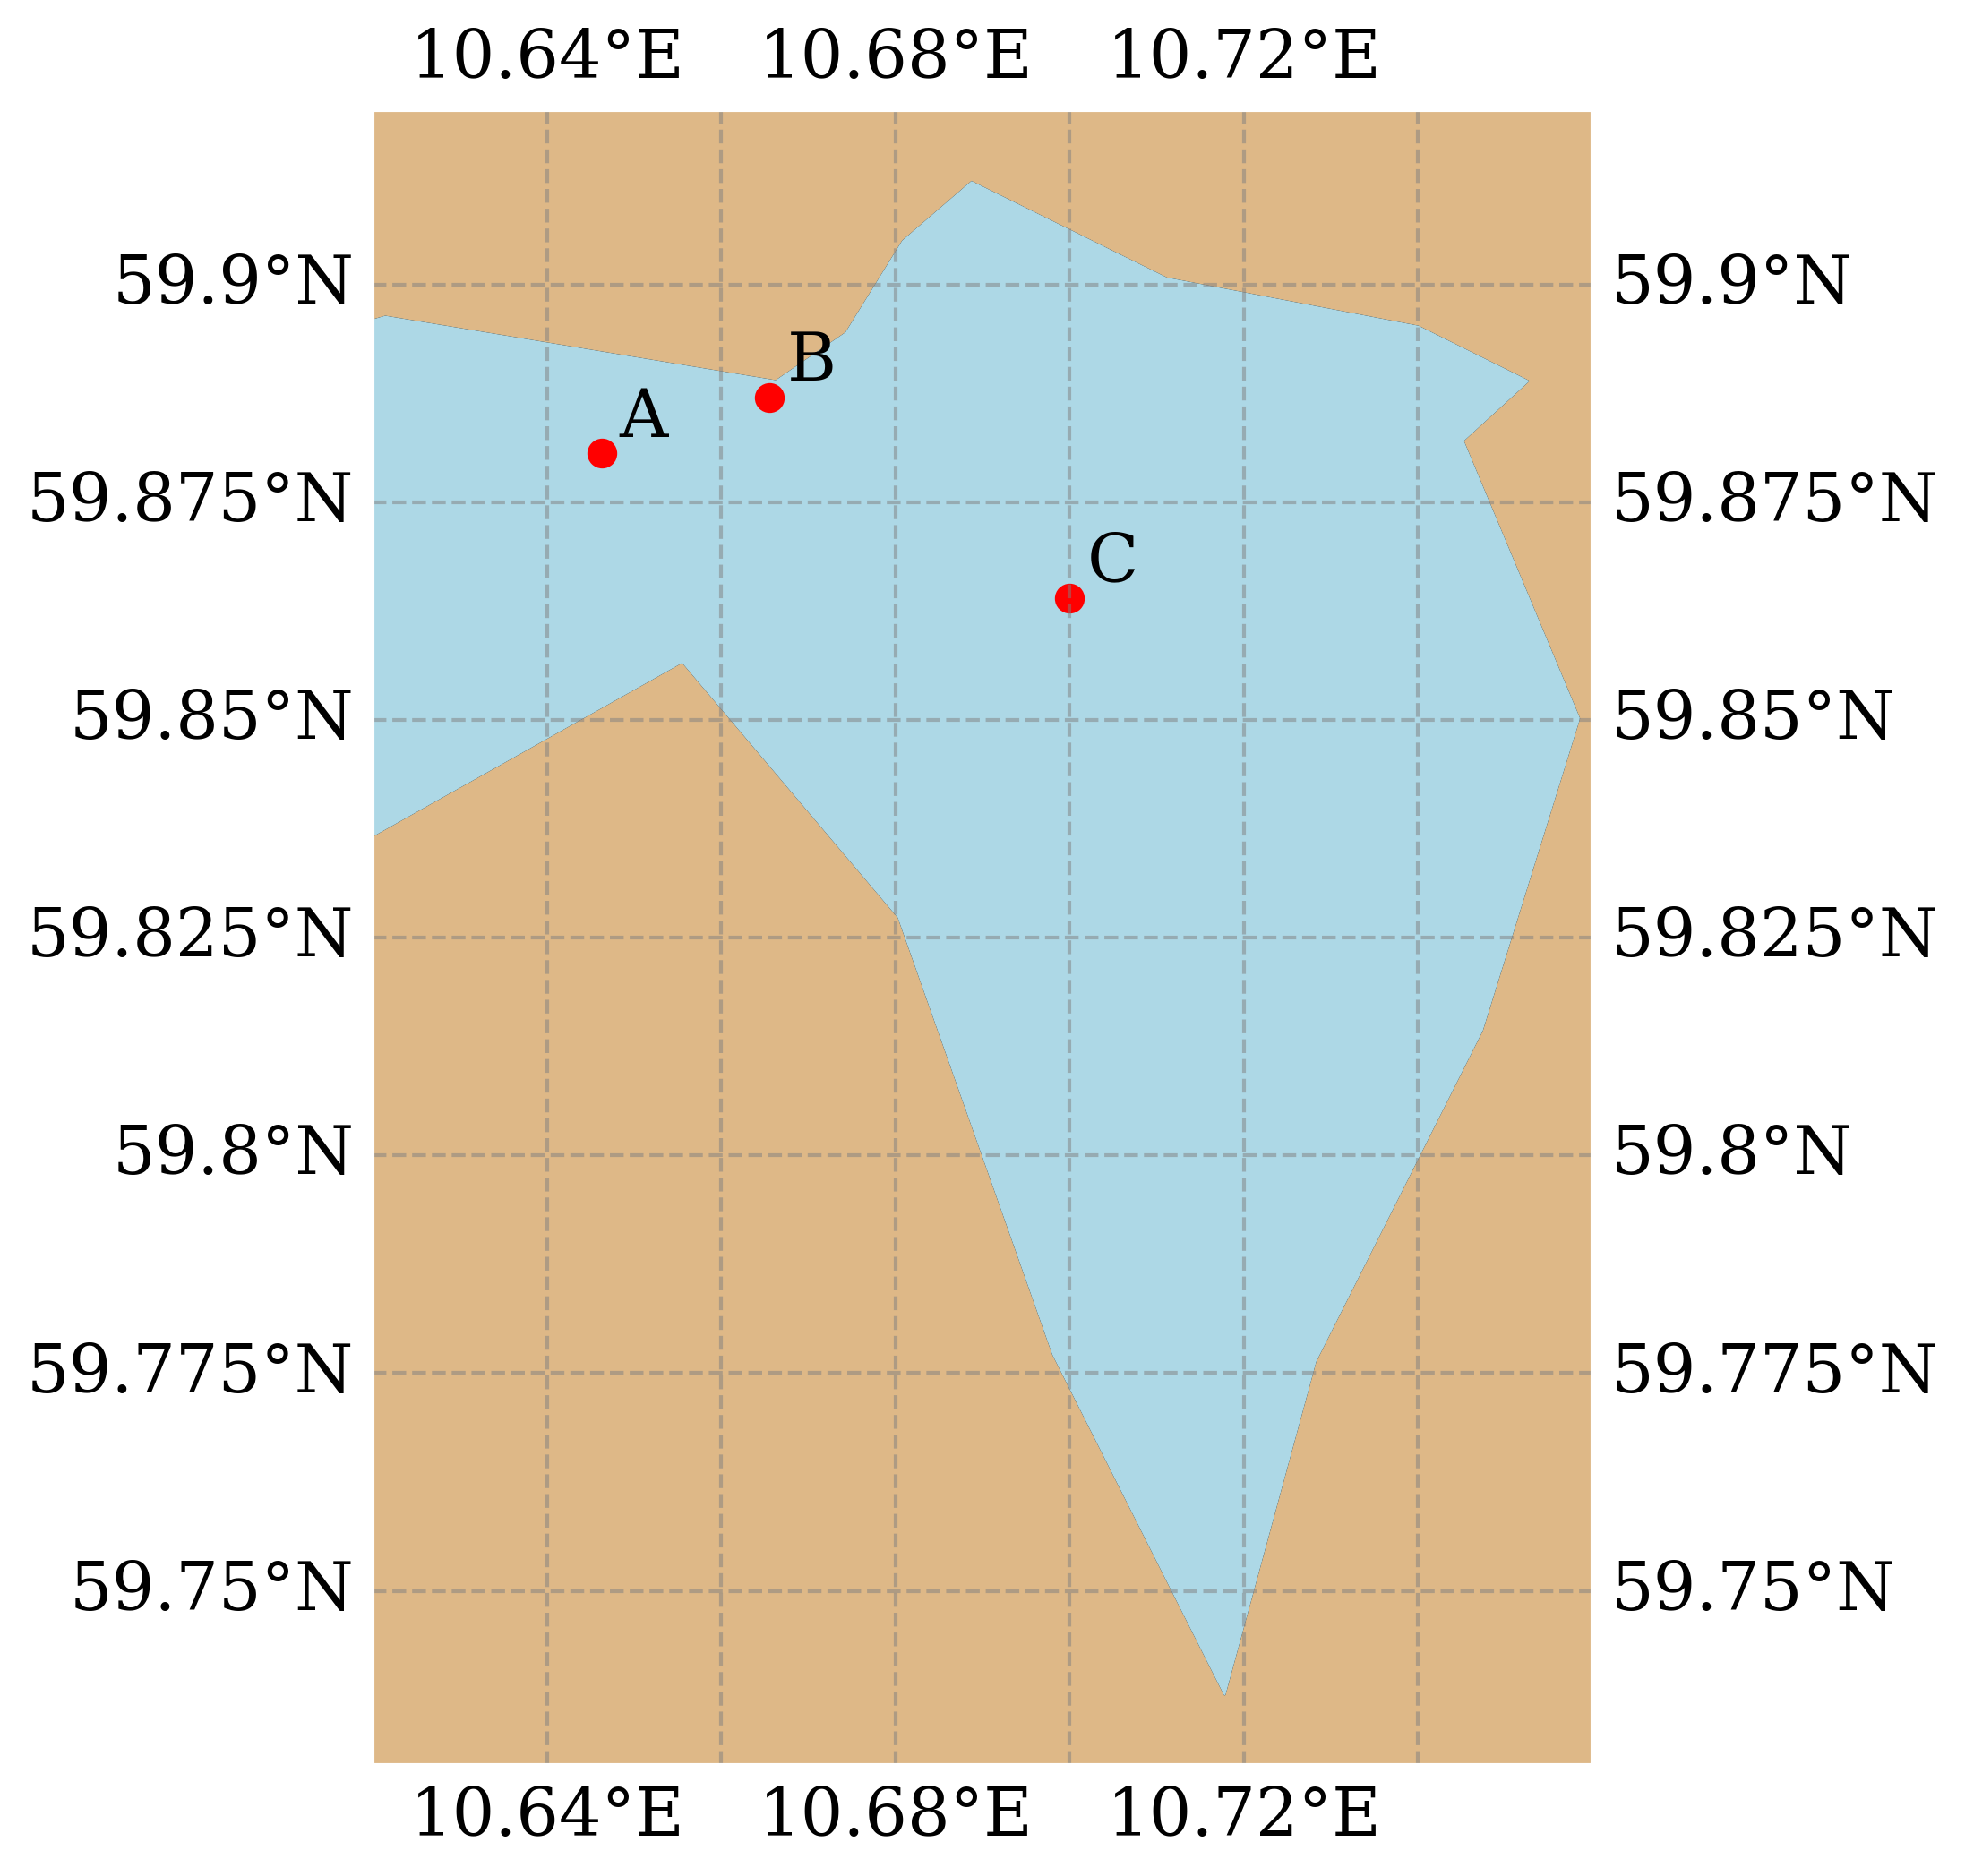
\includegraphics[width=\linewidth]{../figures/station_map_3_stations.png}
        \caption{Three hydrographic measurement locations in the inner Oslo fjord.}
        \label{fig:map_ctd}
\end{wrapfigure}
\newpage
\subsection{CTD measurements}
A CTD measures conductivity, temperature and depth. The conductivity is then used to calculate salinity. CTD measurements where taken at three different locations in the Oslo fjord shown in figure \ref*{fig:map_ctd} during two separate cruises. The morning cruise only gathered CTD data from locations A and C. The afternoon cruise gathered data from all three locations. 

Measurements where in all cases taken with a handheld CastAway CTD attached to a rope that was fed manually by students, and a ship mounted SeaBird CTD. The ship mounted CTD was lowered into the water by the crew using a crane. The water depth was checked by computation with the bridge to avoid the CTD sitting at the bottom. CastAway measurements were limited by the length of the rope.

\subsection{ROMS model}
The model data used is from MET Norway's ROMS (Regional Ocean Modeling System) model. This data was extracted from MET's treadds server.
Salinity and potential temperature data are extracted directly from the model. Due to density data being unavailable, this was calculated using the GSW (Gibbs Seawater) library in Python. Model based profiles are generated for the CTD measurement locations in figure \ref*{fig:map_ctd} on the 28.09.2023. For the time of day, the closest full hour to the measurement times was chosen. The general method for extracting data from ROMS can be found \href{https://github.com/kaihc/GEO2320/blob/main/cruise/extract_salt_temp_roms_from_metno_thredds.ipynb}{here}.


\subsection{Drifters}
Drifter distance traveled is computed using the Geopy library. This with the logged start and finish times are used to compute an average linear velocity. This only looks at the velocity along a straight line between the two points and does not take into account the actual drifter path. Two drifters were equipped with GPS trackers to log the full path.

\subsection{Sea-air fluxes}
For the computation of fluxes data was collected from panels on the bridge. The following parameters were noted:
\begin{enumerate}[label=--, itemsep=0pt,parsep=0pt]
        \item wind speed and direction (m/s and degrees clockwise from N),
        \item relative humidity (\%),
        \item sea surface temperature (C),
        \item air temperature (C),
        \item mean sea level pressure (hPa).
\end{enumerate}

Additionally, significant wave height (in meters) and total cloud cover (in oktas) were taken by manual observation. A note was also made if it was raining.

These parameters are then used as input for the COARE 3.5 model to compute bulk long- and shortwave as well as sensible- and latent heat fluxes. The COARE script can be found \href{https://github.com/kaihc/GEO2320/blob/main/cruise/airsea_data.ipynb}{here}.

\subsection{Secchi disc}
A Secchi disc is a white disk attached to the end of a rope. This can be lowered into the water to assess the waters turbidity or transparency. The disk is lowered slowly until it is no longer visible, this depth is the `'`Secchi depth''. For a more accurate result, the disk was lowered twice with several students observing it. Each student kept their Secchi depth to themselves until the experiment was over. The average of these is then taken as the actual Secchi depth. 


\section{Results}\label{sec:results}
\setlength{\intextsep}{12pt}


\subsection{CTD Profiles}
Data was successfully gathered for locations A and C in figure \ref*{fig:map_ctd} on both the morning ang afternoon cruise. Data from location B was unfortunately only gathered in the afternoon. This section will therefore focus on locations A and C. Exact location coordinates and timestamps for all profiles can be found in appendix \ref*{app:CTD} and \ref*{app:model}.

\begin{figure}[H]
    \begin{adjustwidth}{-2.5cm}{-2.5cm}  % Adjust the values to change the margins
    \begin{subfigure}{0.65\textwidth}
            \centering
            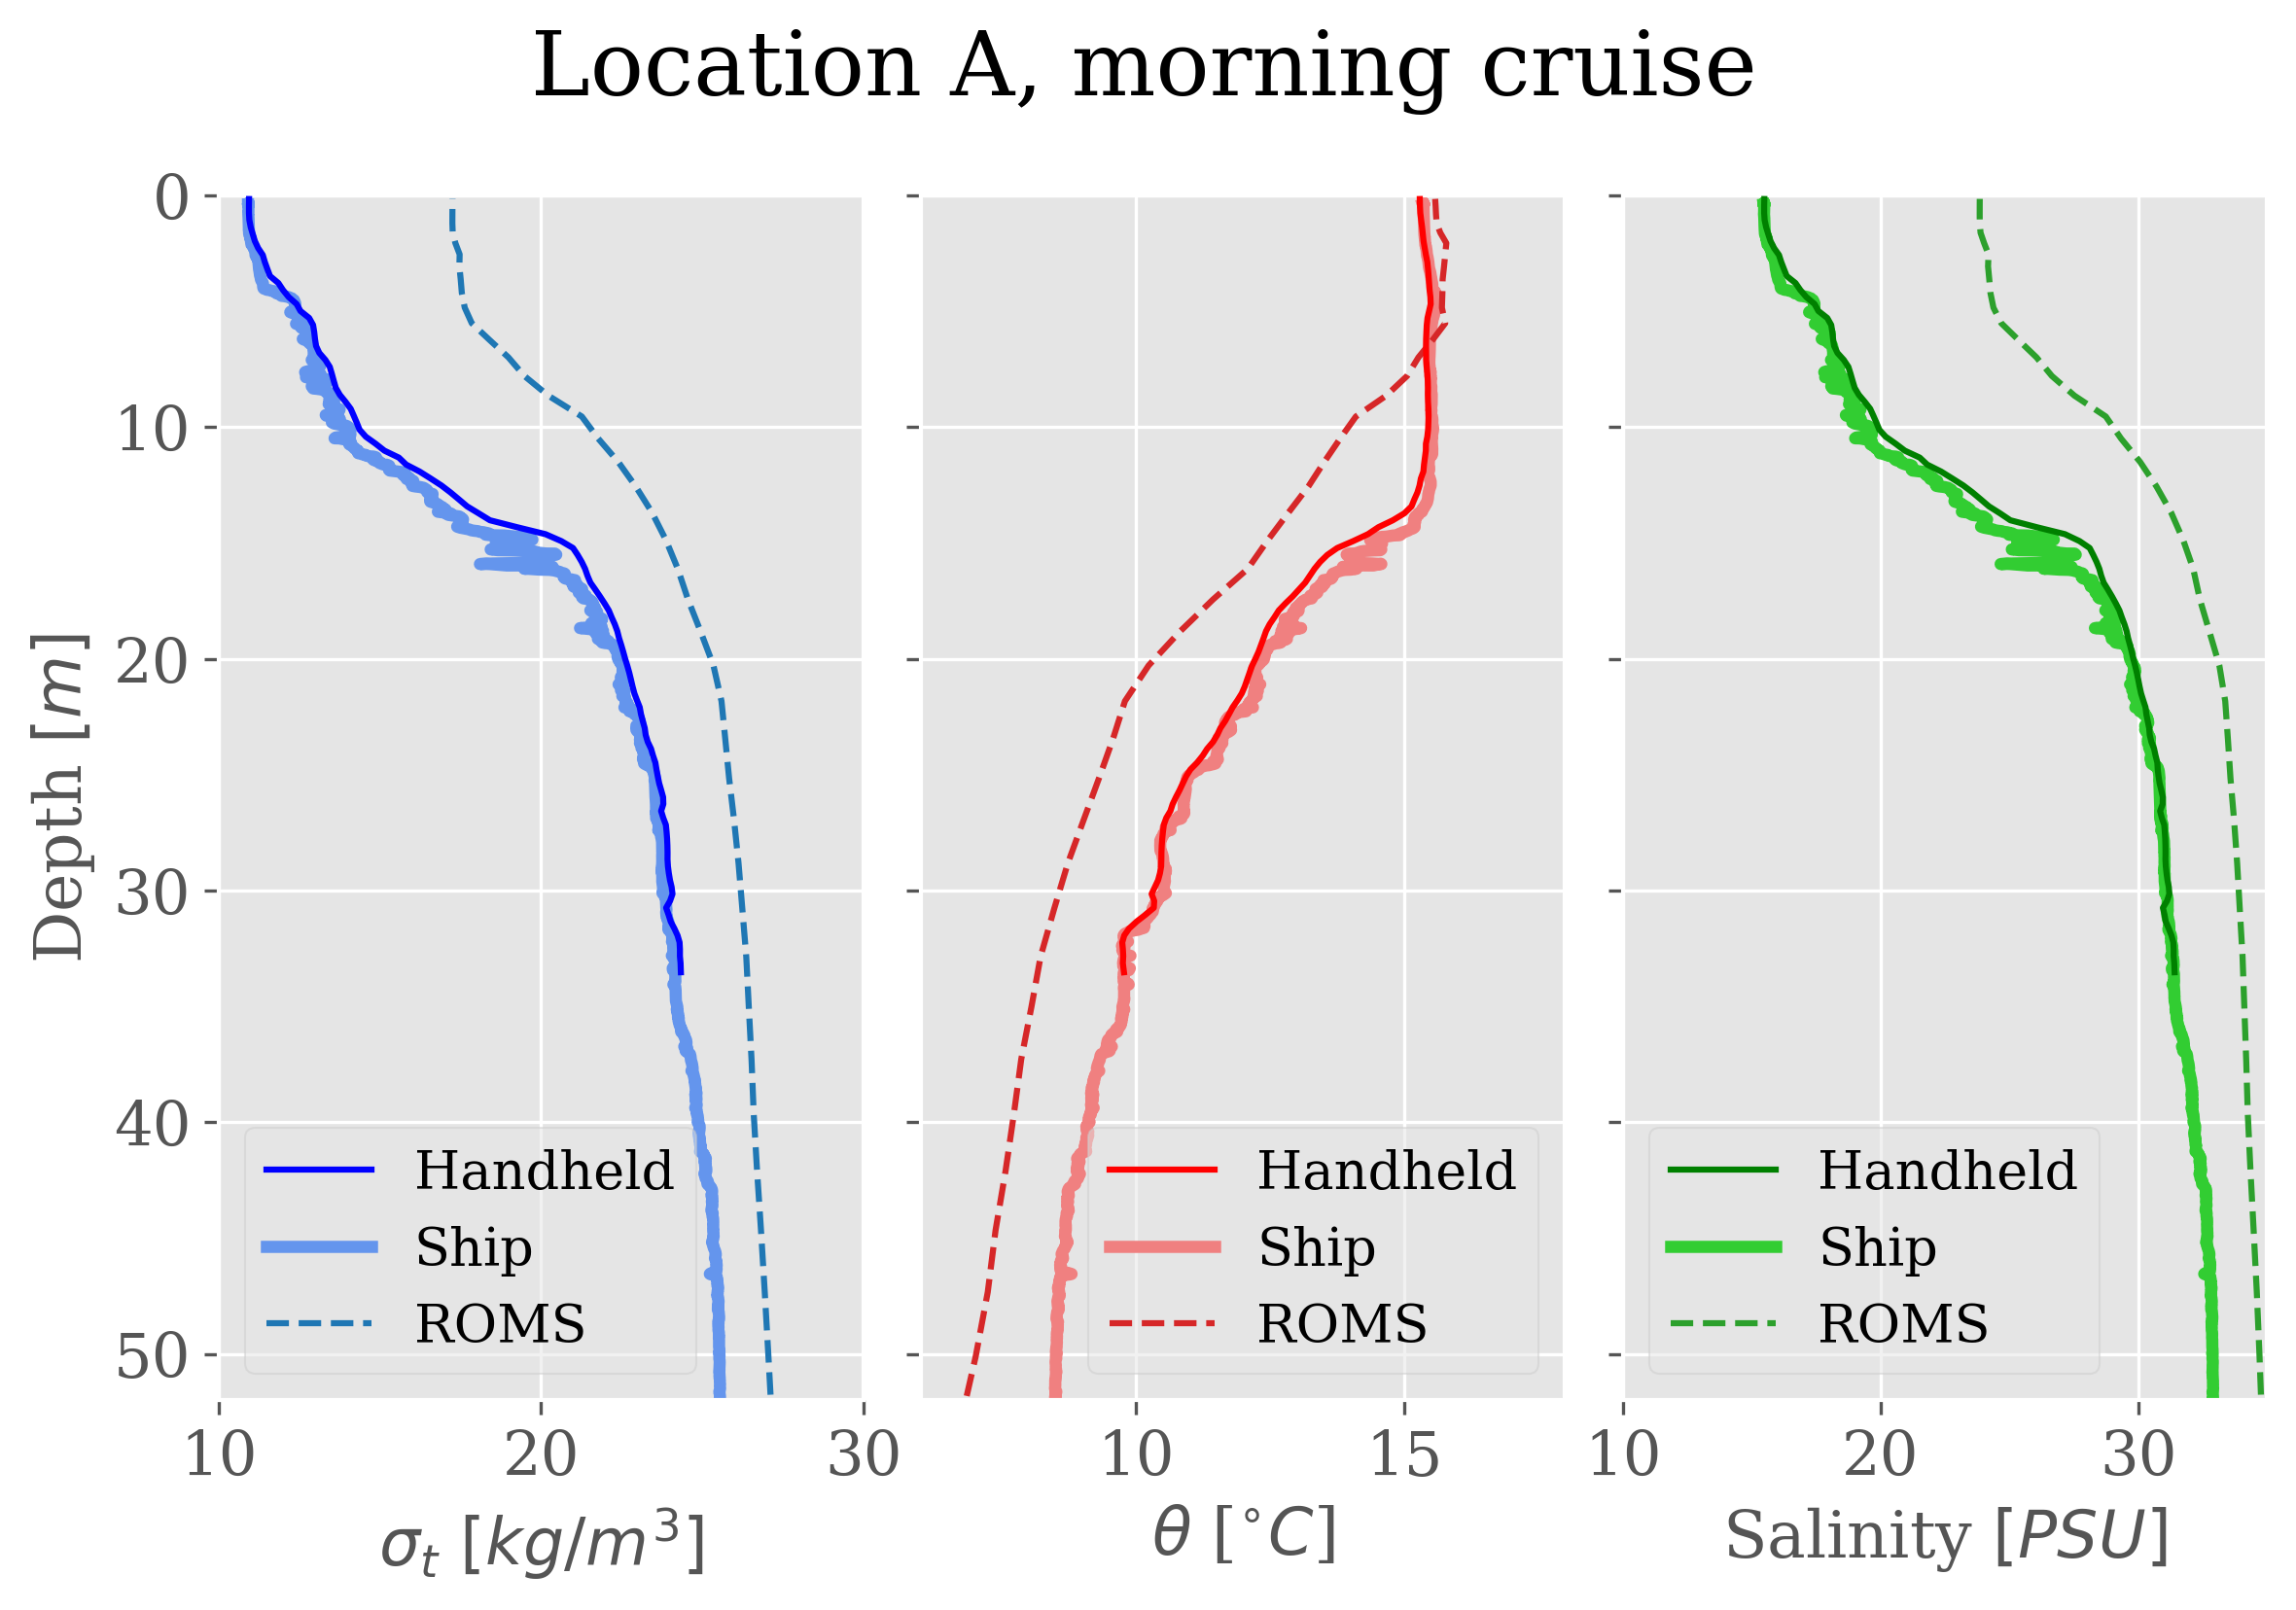
\includegraphics[width=1.\linewidth]{../figures/combined_profiles/Location_A_morning_cruise.png}
            \caption{}
            \label{fig:morning_A}
    \end{subfigure}%
    \begin{subfigure}{0.65\textwidth}
            \centering
            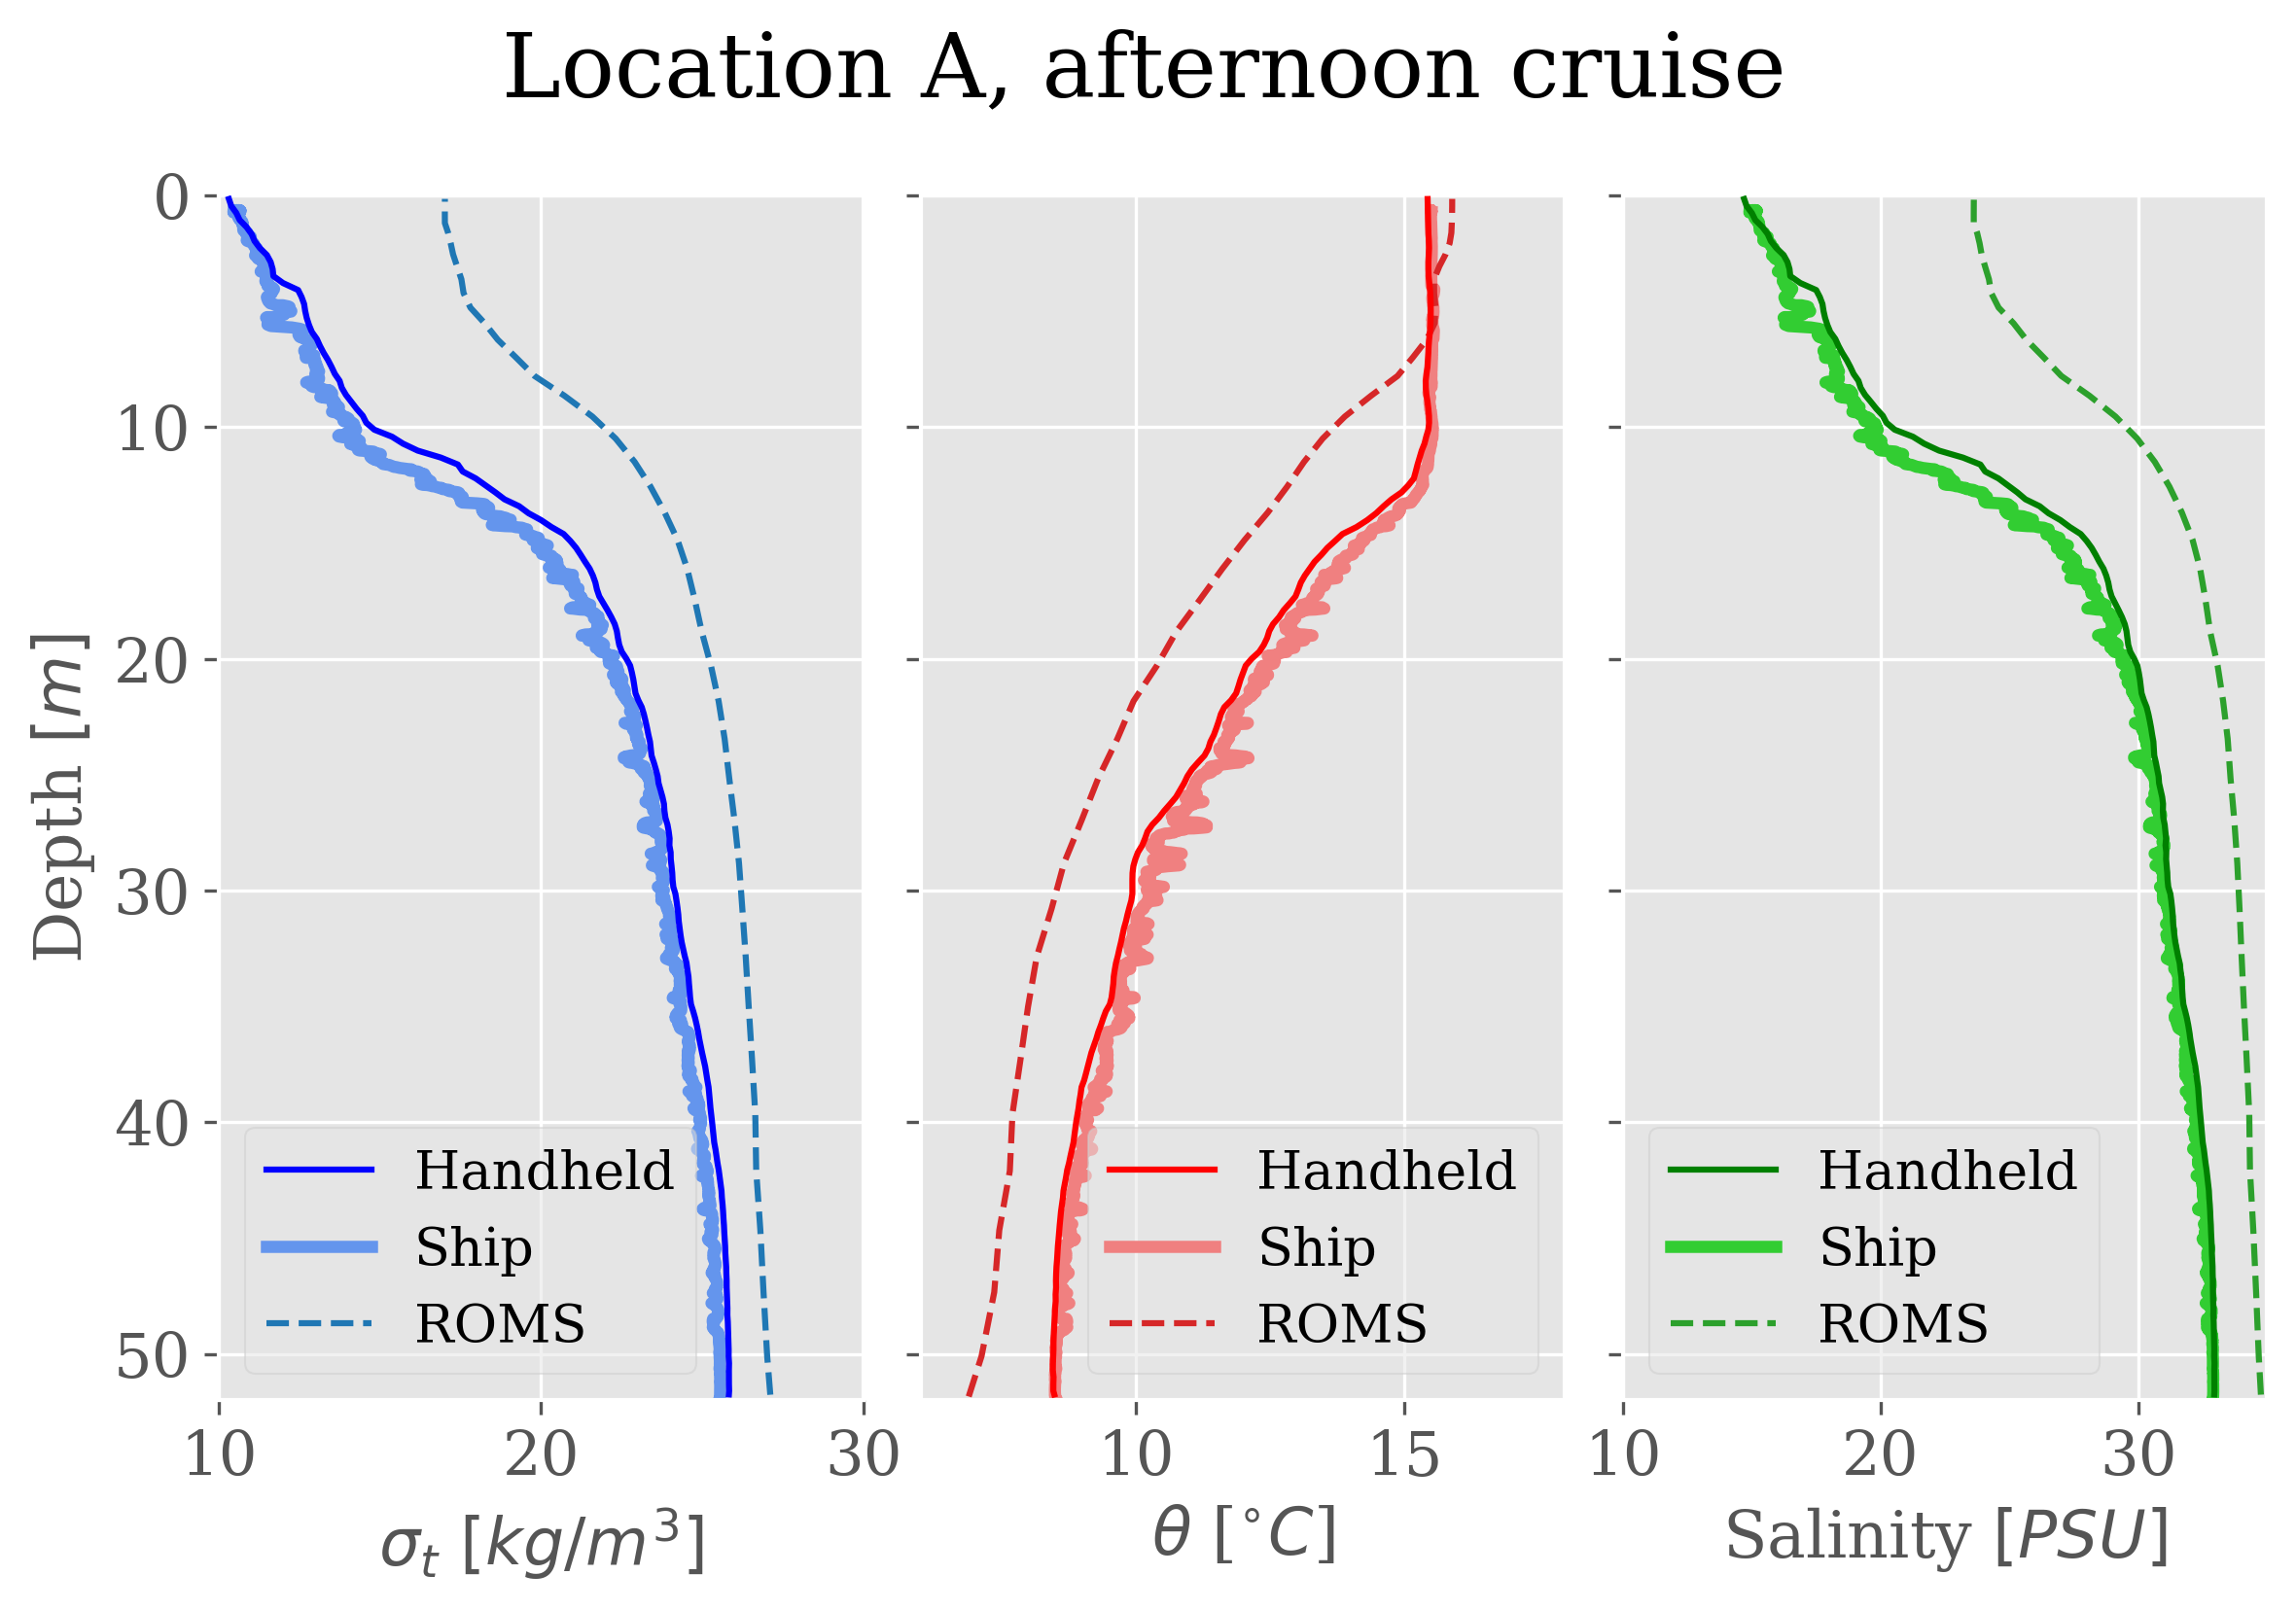
\includegraphics[width=1.\linewidth]{../figures/combined_profiles/Location_A_afternoon_cruise.png}
            \caption{}
            \label{fig:afternoon_A}
    \end{subfigure}
    \end{adjustwidth}
    
    \caption{Depth profile of potential density, potential temperature and salinity at location A from handheld and ship CTDs as well as the ROMS model}
    \label{fig:location_A}
\end{figure}

\begin{figure}[H]
    \begin{adjustwidth}{-2.5cm}{-2.5cm}  % Adjust the values to change the margins
    \begin{subfigure}{0.65\textwidth}
            \centering
            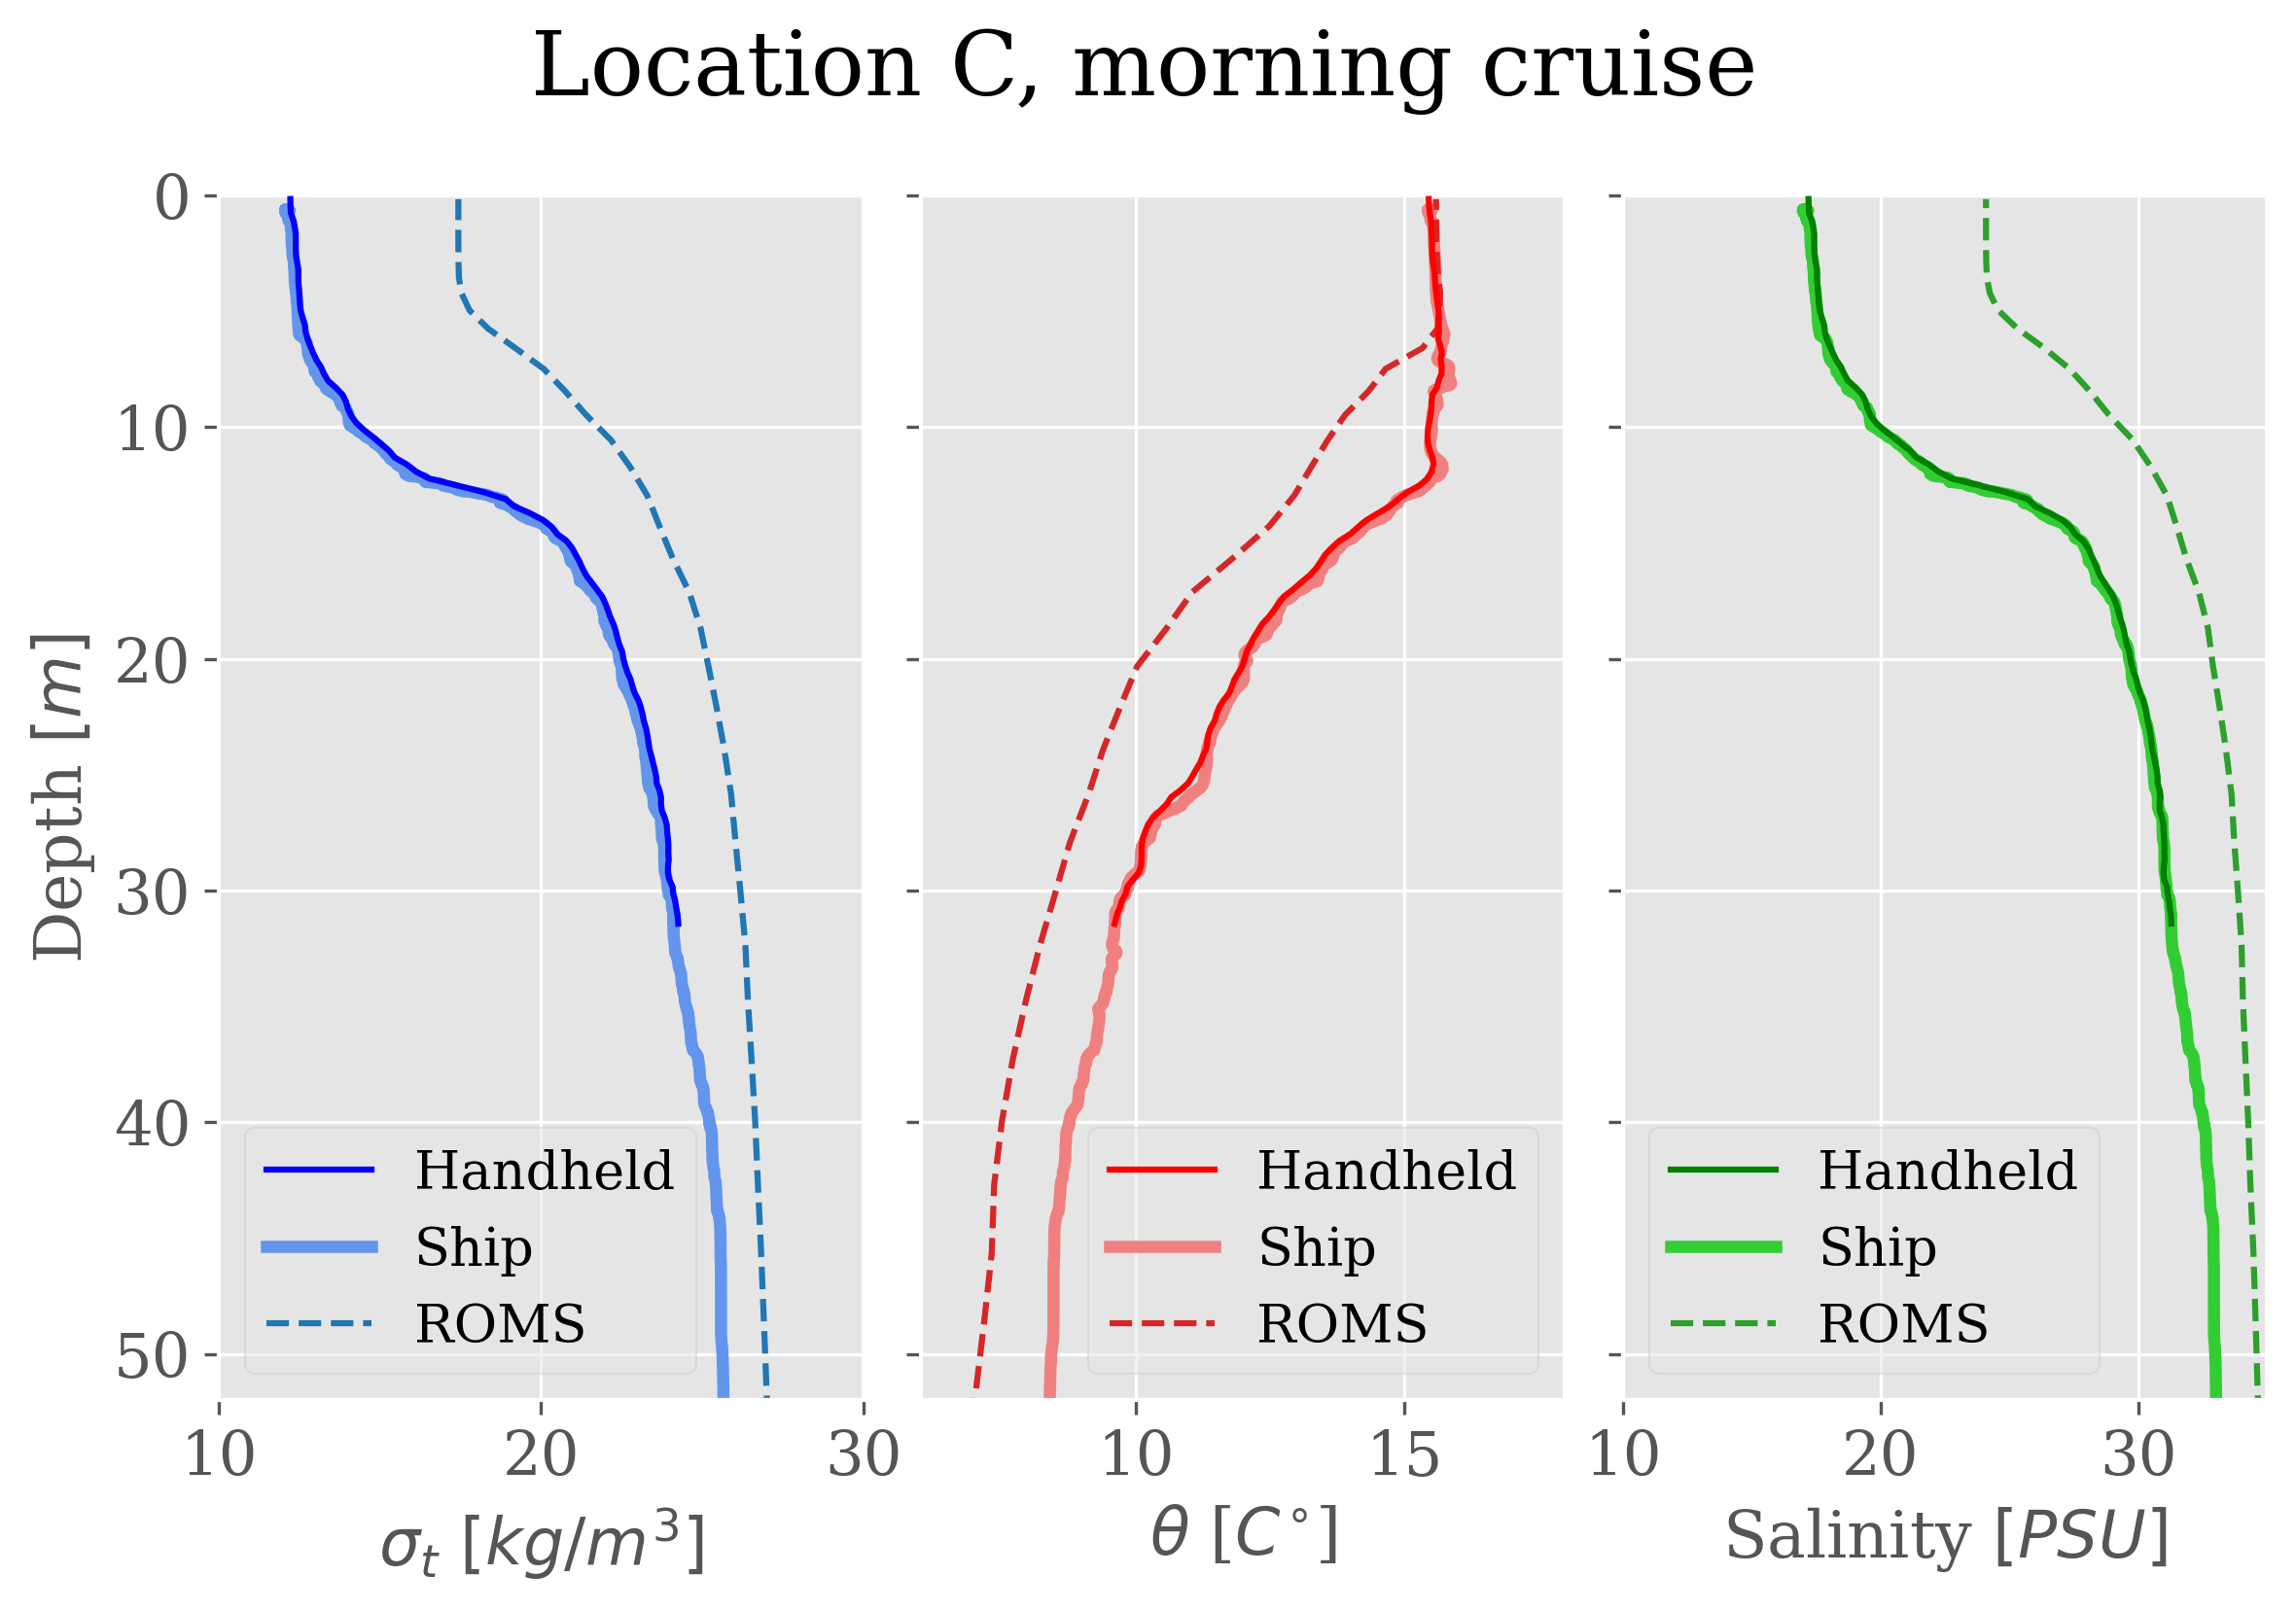
\includegraphics[width=1.\linewidth]{../figures/combined_profiles/Location_C_morning_cruise.png}
            \caption{}
            \label{fig:morning_C}
    \end{subfigure}%
    \begin{subfigure}{0.65\textwidth}
            \centering
            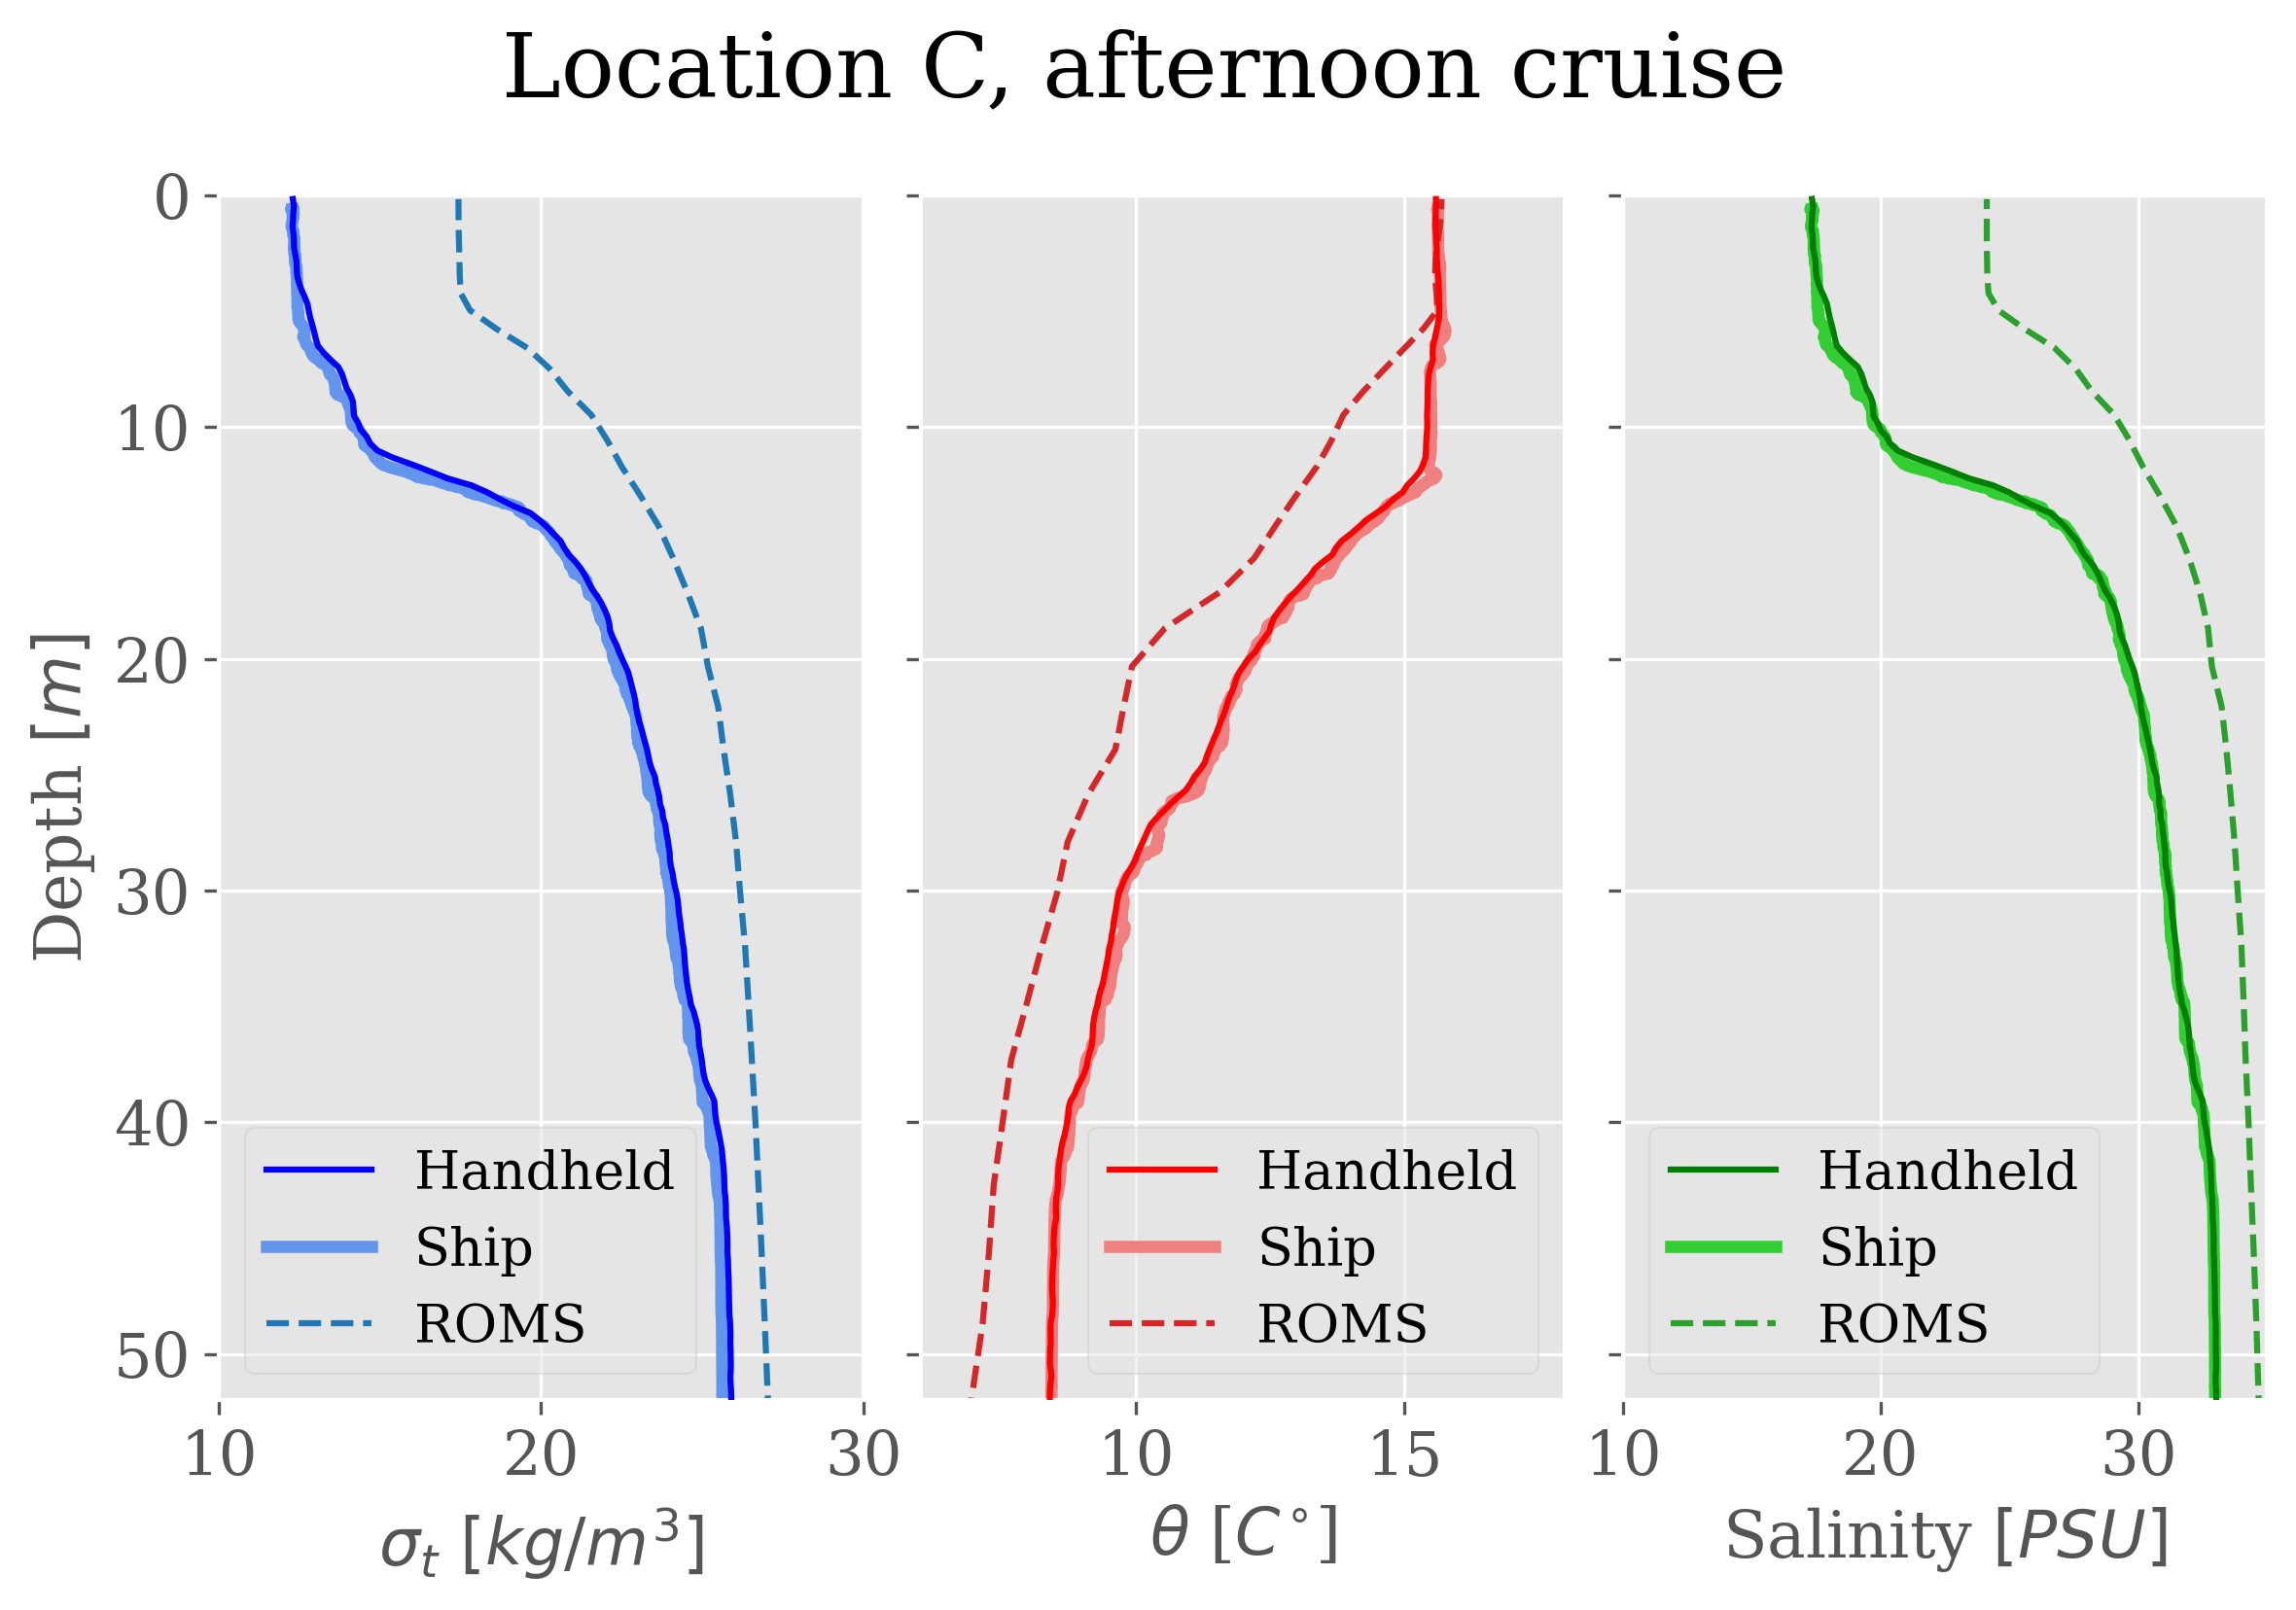
\includegraphics[width=1.\linewidth]{../figures/combined_profiles/Location_C_afternoon_cruise.png}
            \caption{}
            \label{fig:afternoon_C}
    \end{subfigure}
    \end{adjustwidth}
    
    \caption{Depth profile of potential density, potential temperature and salinity at location C from handheld and ship CTDs as well as the ROMS model}
    \label{fig:location_C}
\end{figure}

\newpage
Figure \ref*{fig:location_A} shows depth profiles for location A in figure \ref*{fig:map_ctd} with \ref*{fig:morning_A} showing results from the morning cruise and \ref*{fig:afternoon_A} for the afternoon. Blue lines show potential density data, red is potential temperature and green is salinity. In each profile, the thinner dark line shows results from the handheld CTD, the lighter and thicker line shows results from the ship mounted CTD and the dashed line shows results from MET Norway's ROMS model. Figure \ref*{fig:location_C} shows equivalent results for location C.

The handheld and ship CTD data agrees very well, especially in location C. In location A, the ship CTD shows slightly lower values and more noise than the handheld profile for potential density and salinity. It also has more noise but shows higher values for potential temperature below 10 m. 

The ROMS model replicates the shape of the potential temperature and salinity profiles well but has a positive bias for salinity. Notably this bias decreases with depth. For the potential temperature the ROMS model matches the observational data well for the first 5-7 m, but then has a negative bias for deeper values. The plotted potential density for ROMS is not considered since this is computed separately based on model salinity and potential temperature, and not actual model density data.

All profiles show a similar shape with the greatest change in the observed parameter occurring between 10 and 15 m of depth.

There are some minor changes in the top few meters when comparing morning and afternoon measurements. For location A, surface potential density and salinity decrease from morning to afternoon whereas potential temperature increases. For location C, all three parameters show a very slight increase in the uppermost layer.

Comparing locations A and C, A is more stratified in the top 10 m, whereas C seems to have a relatively well mixed homogeneous top layer. Below 20 m the locations are very similar.

\subsection{Drifters}

% drifters 
\begin{figure}[H]
    % \begin{adjustwidth}{-2.5cm}{-2.5cm}  % Adjust the values to change the margins
    \begin{subfigure}{0.5\textwidth}
            \centering
            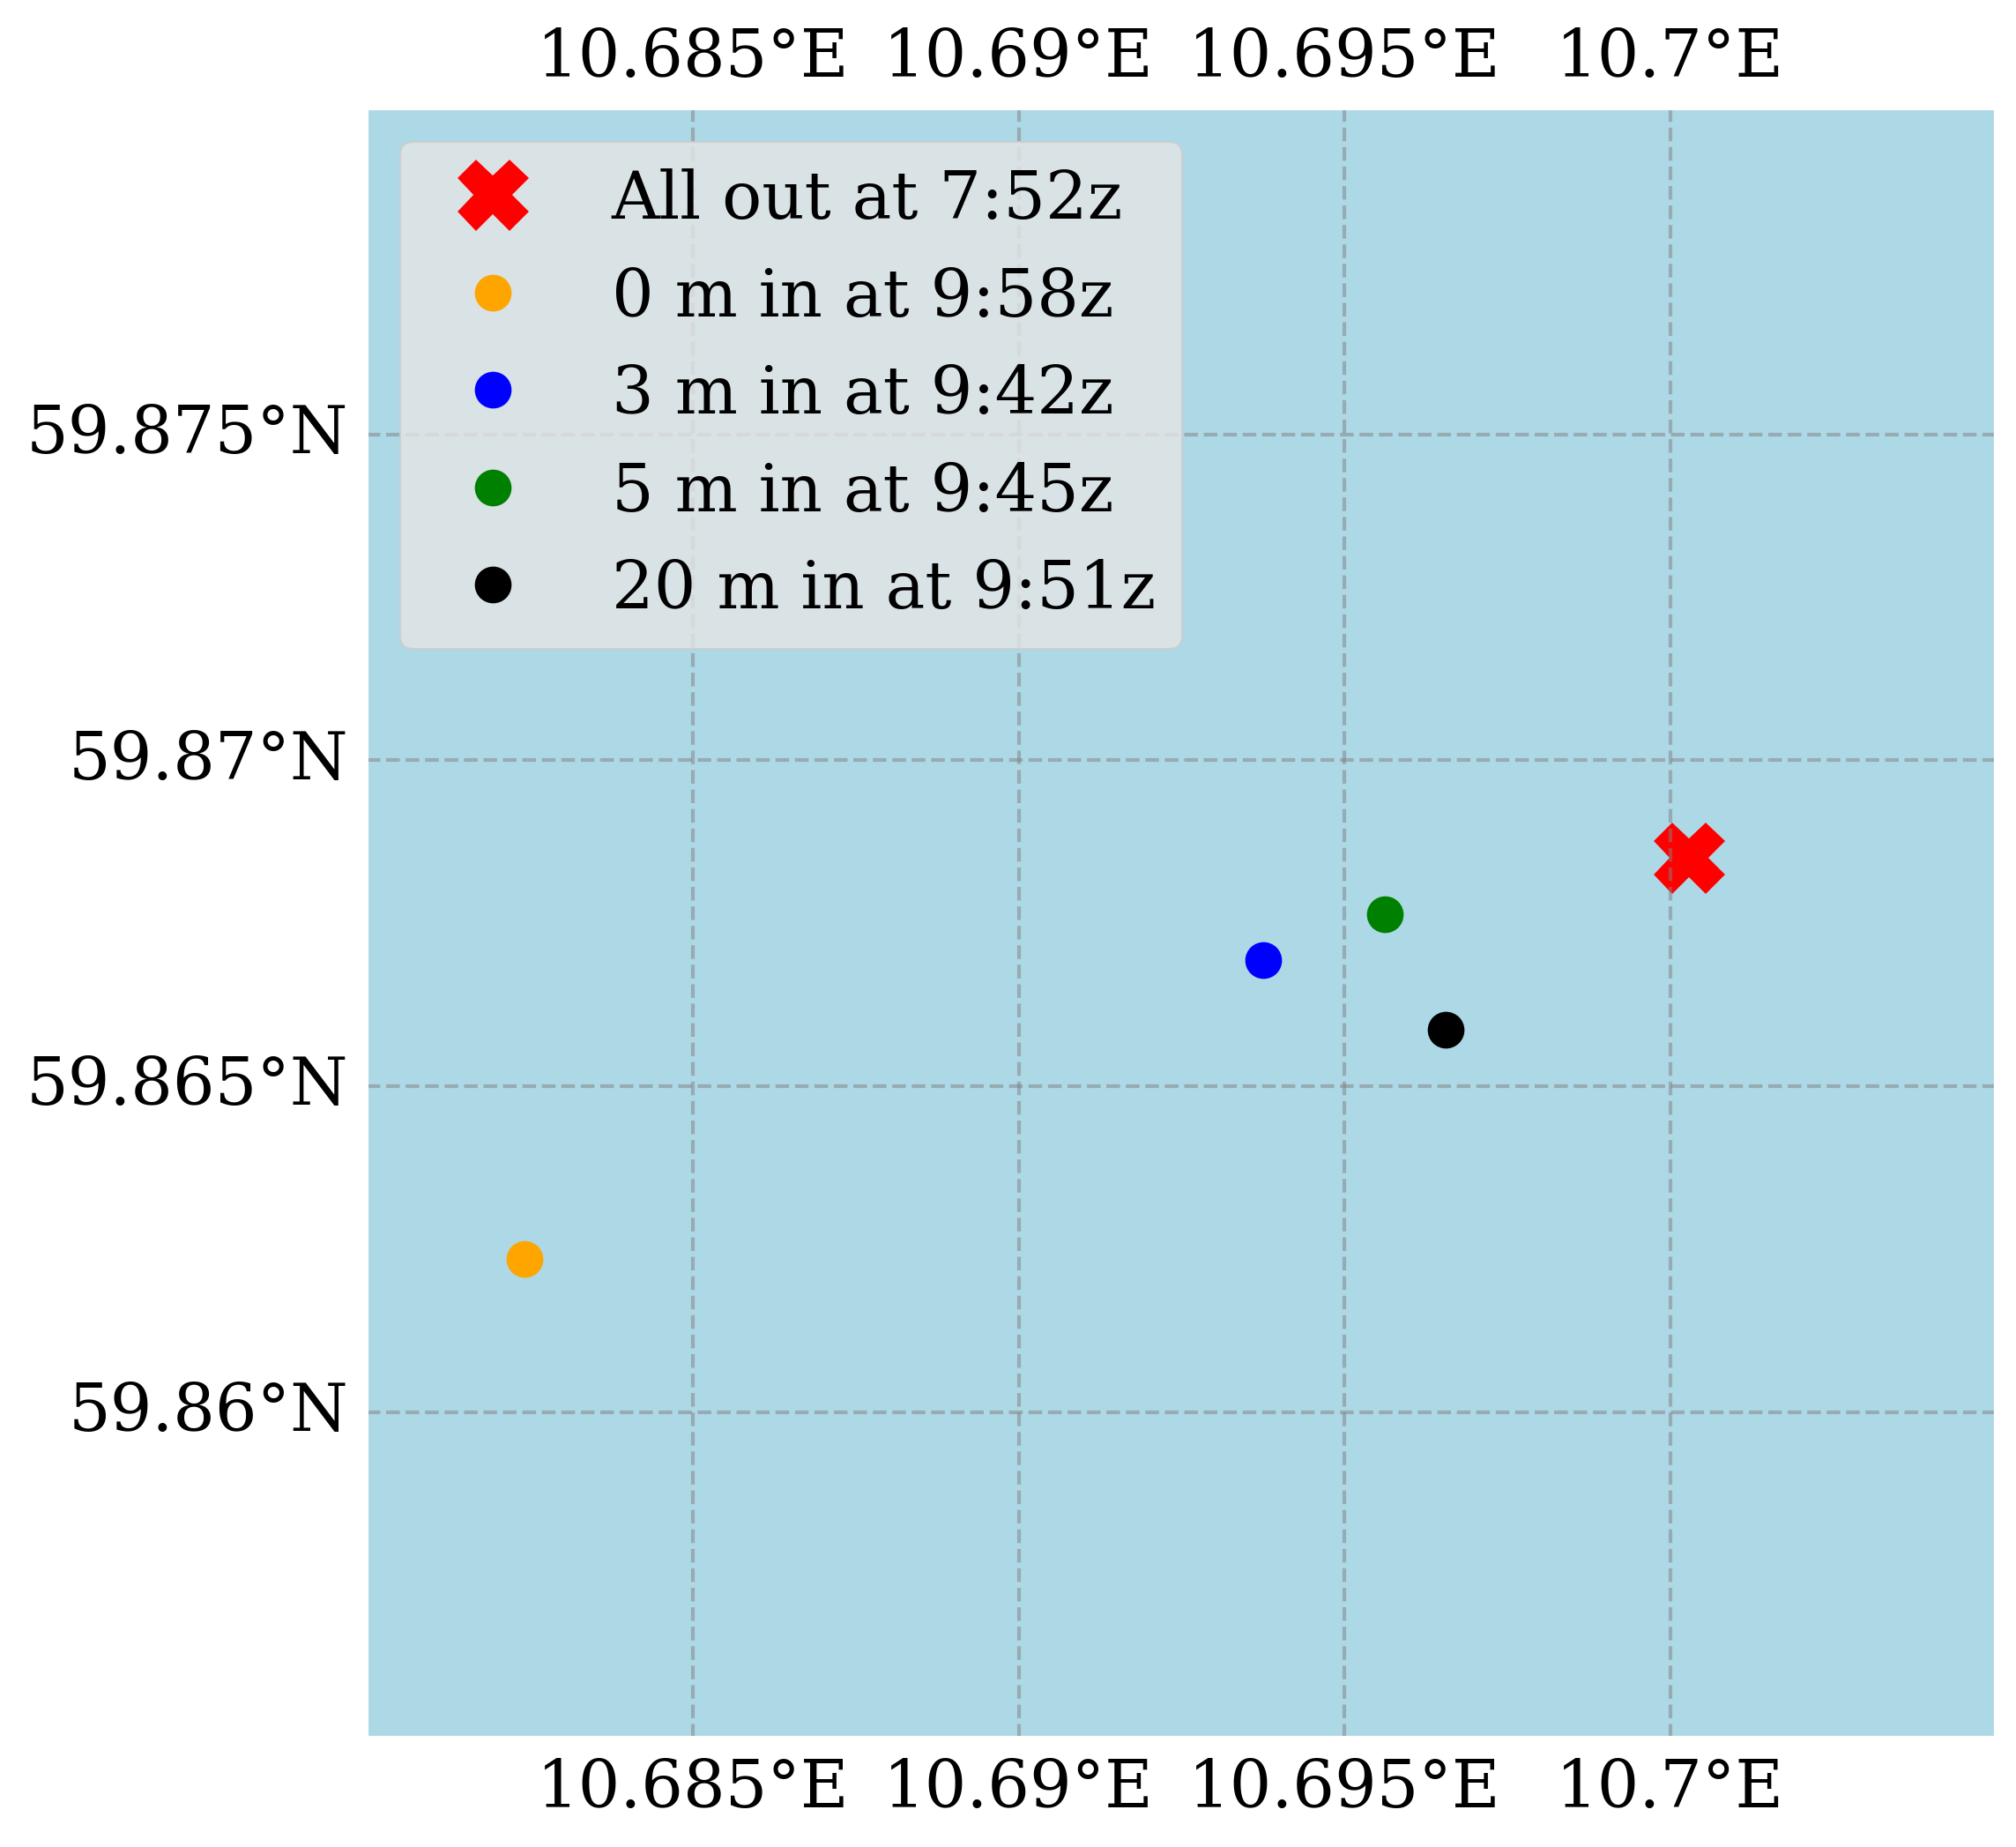
\includegraphics[width=1.\linewidth]{../figures/drifters/drifters_tokt1.png}
            \caption{Morning cruise}
            \label{fig:drifter_1}
    \end{subfigure}%
    \begin{subfigure}{0.5\textwidth}
            \centering
            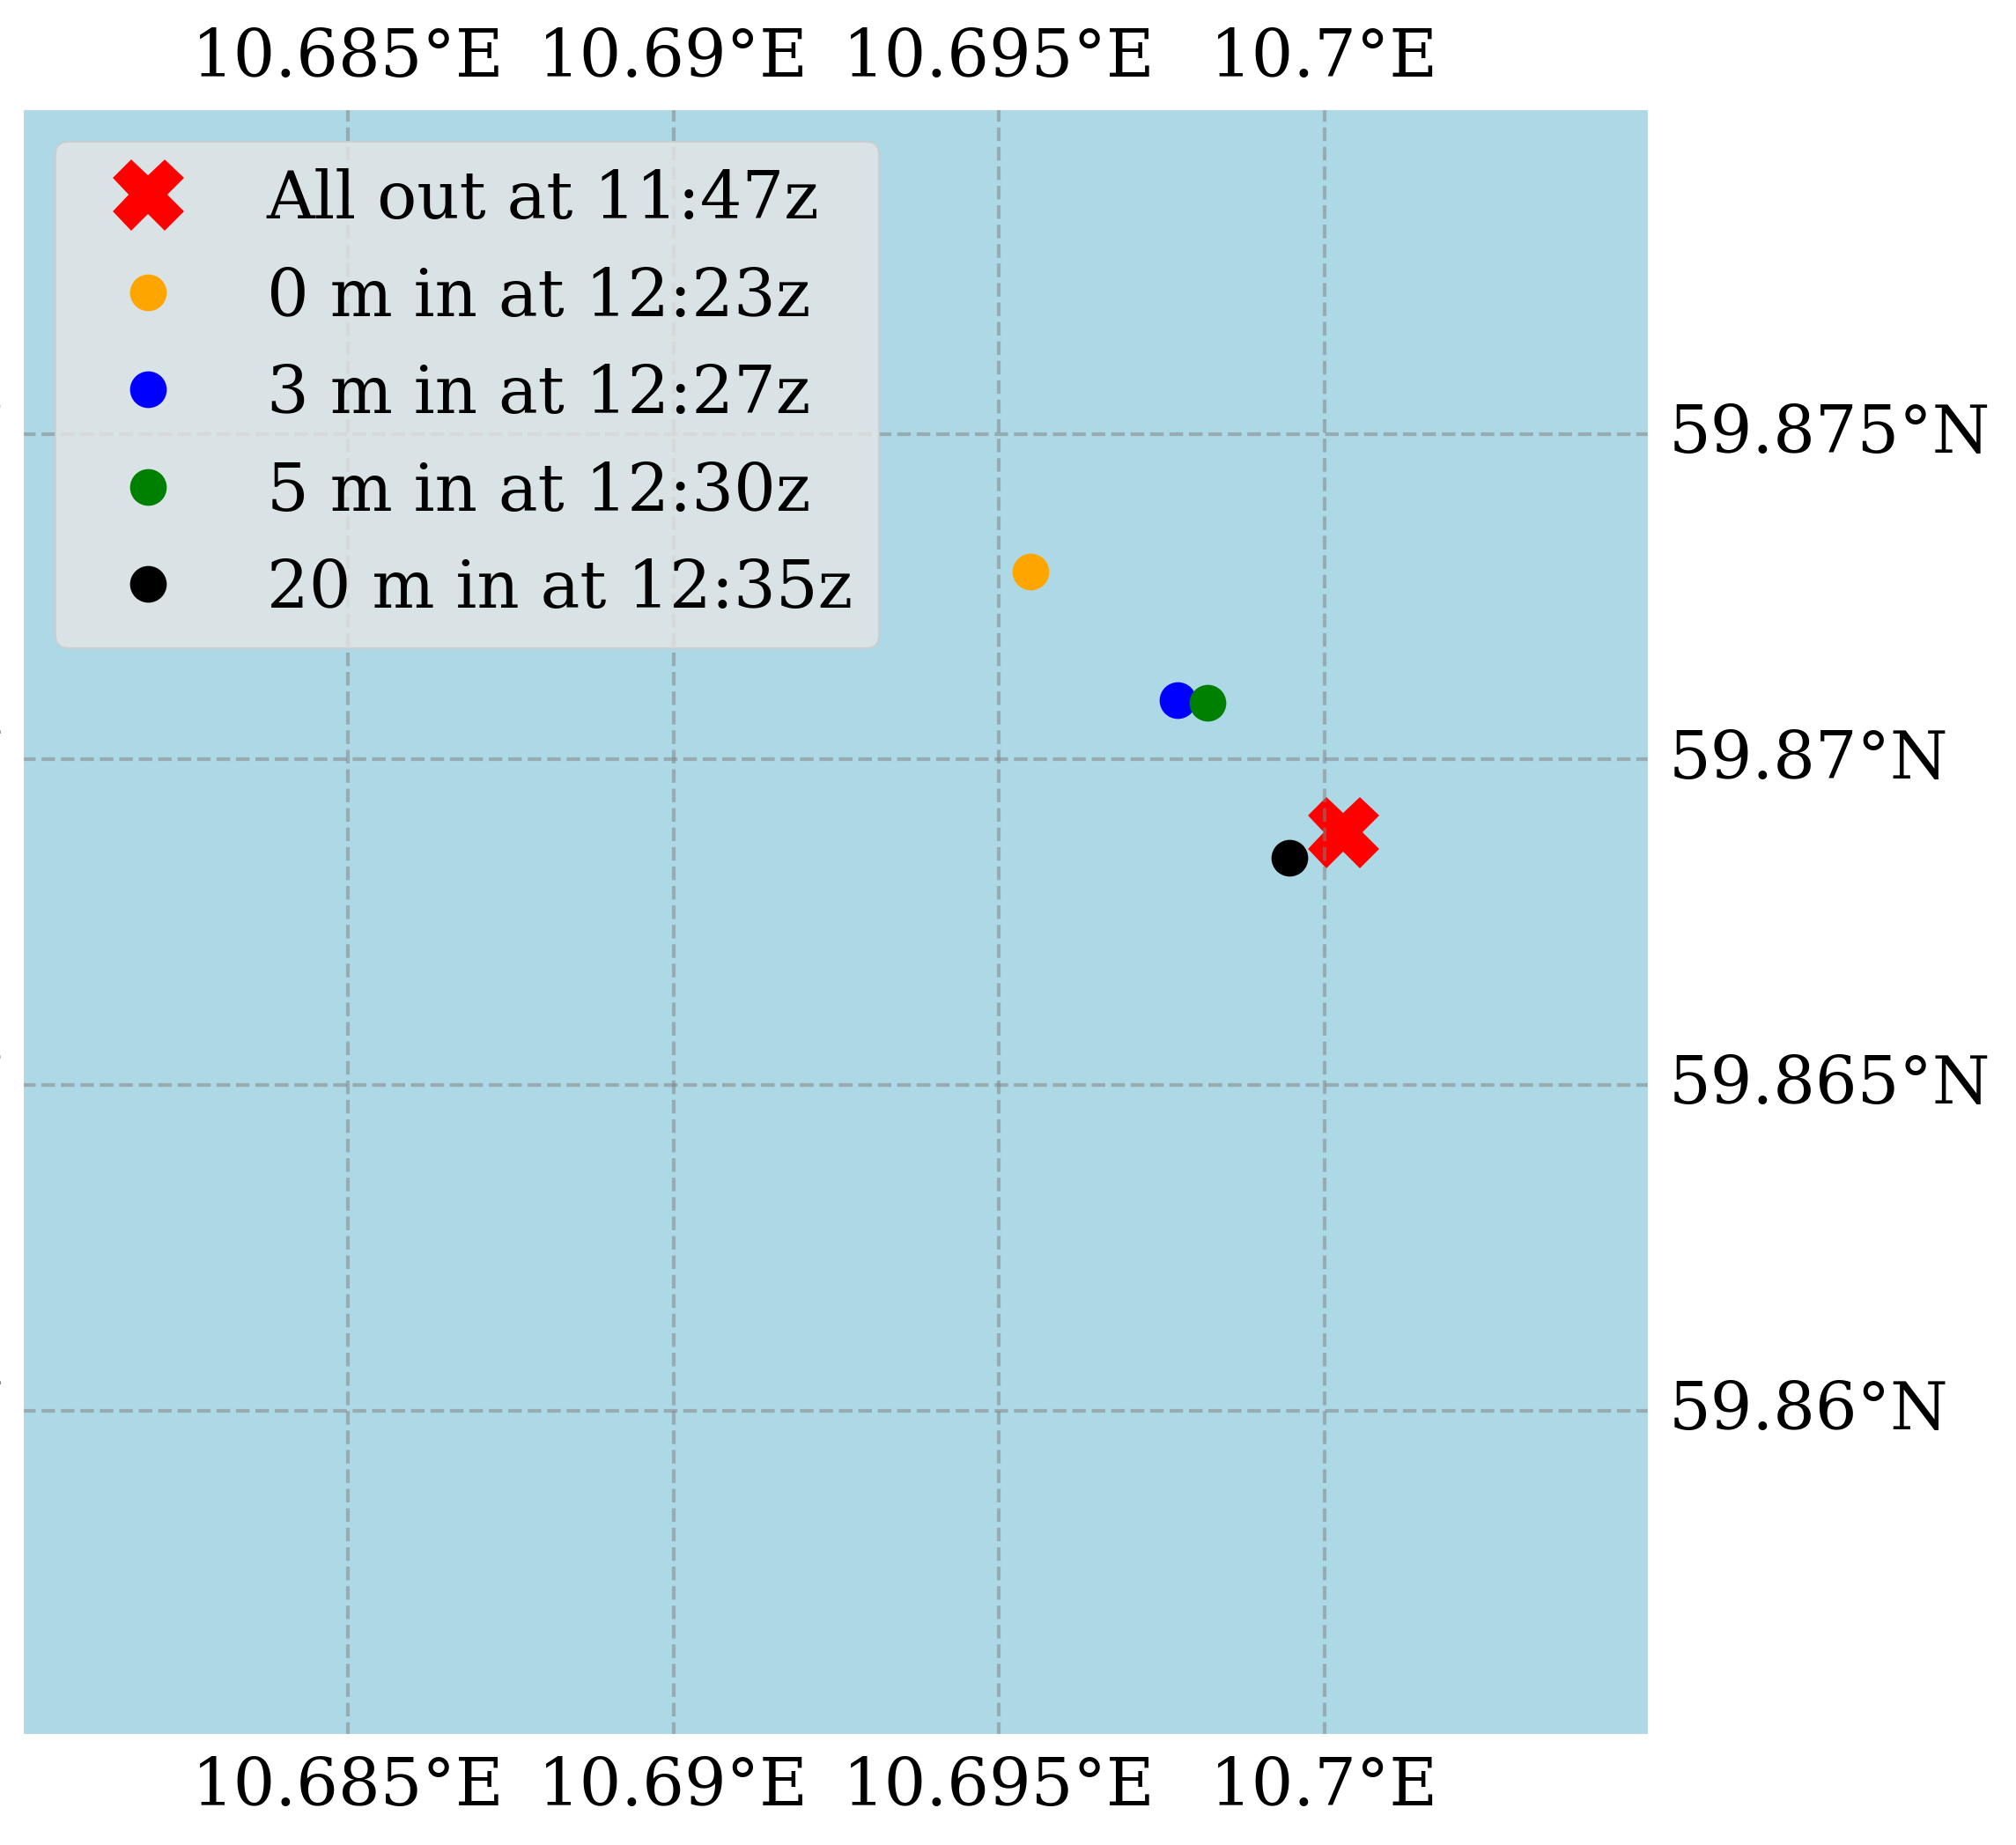
\includegraphics[width=1.\linewidth]{../figures/drifters/drifters_tokt2.png}
            \caption{Afternoon cruise}
            \label{fig:drifter_2}
    \end{subfigure}
    % \end{adjustwidth}
    
    \caption{Start and end locations for four drifters with drogues at different depths. The red cross marks the joint starting location for all four drifters. Dots mark the stop/collection points. The same four drifters were released in tho morning (\ref*{fig:drifter_1}) and afternoon (\ref*{fig:drifter_2})}
    \label{fig:drifters}
\end{figure}

Figure \ref*{fig:drifters} shows the start and end positions of four drifters with drogues at different depths (0m, 3m, 5m and 20m). Figure \ref*{fig:drifter_1} shows results from the morning cruise and figure \ref*{fig:drifter_2} the afternoon. Most notably, the yellow drifter with the 0m drogue travels furthest from the starting position (red cross) in both cases. The other three do not drift as far and remain closer together.

% drifter tracks
\begin{figure}[H]
        \centering
        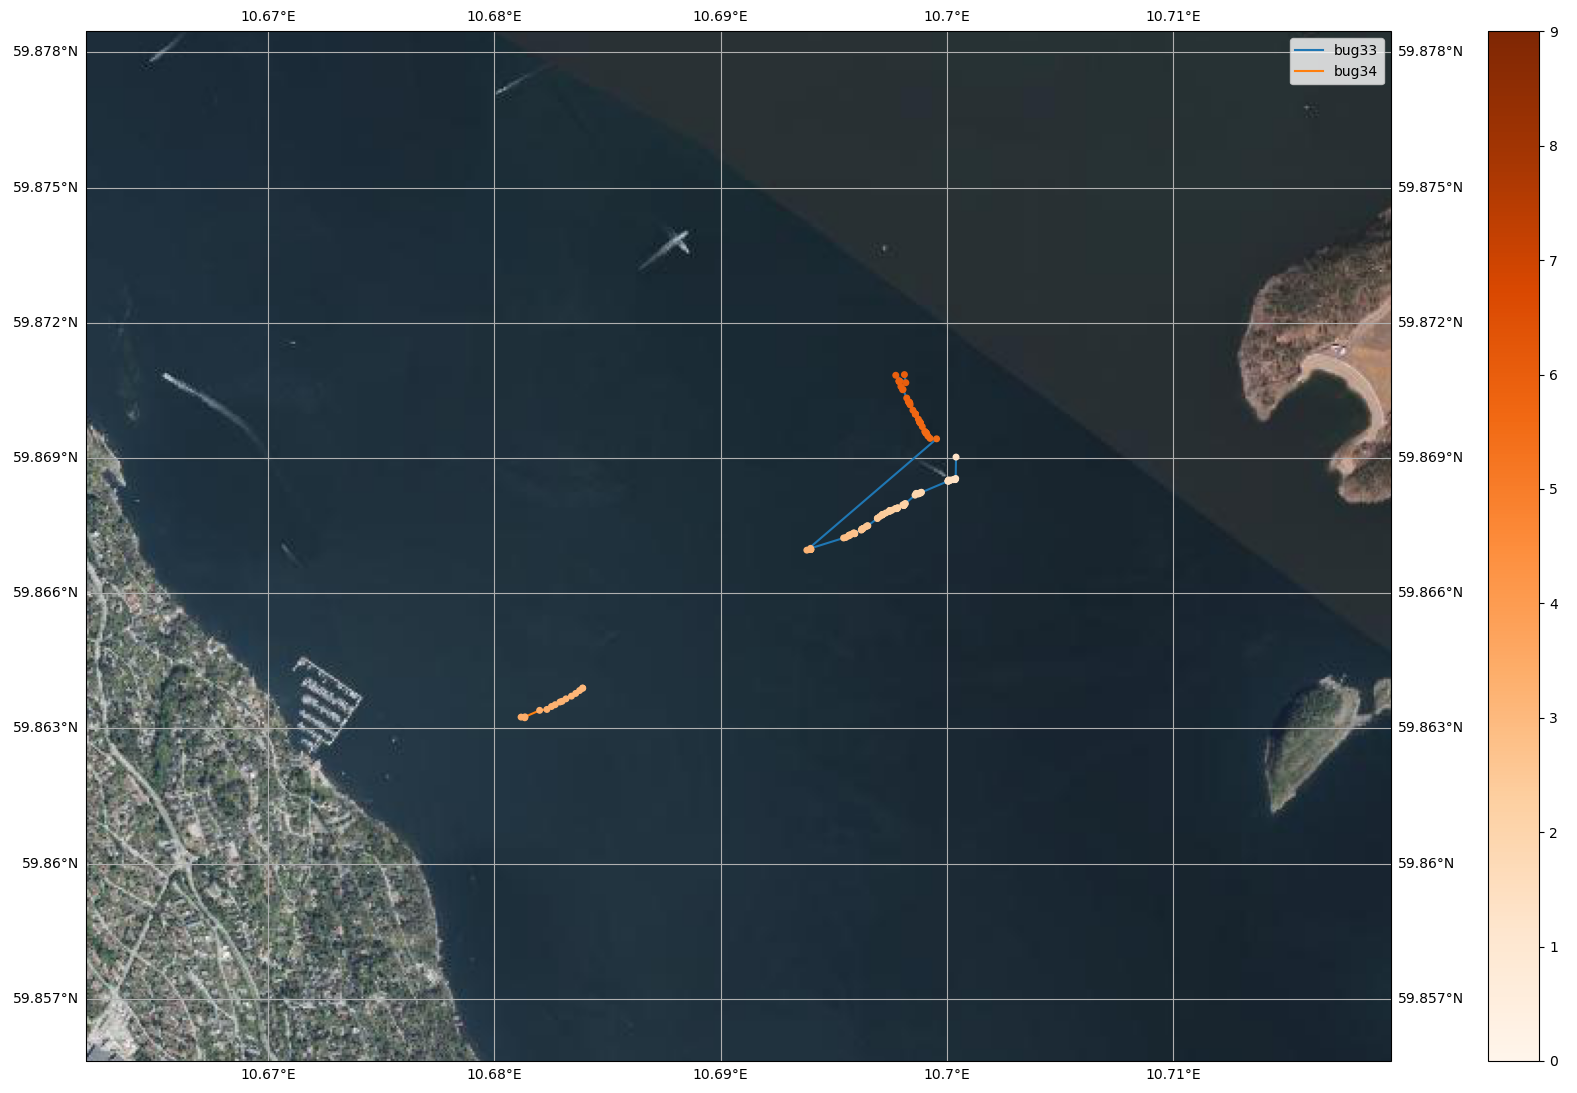
\includegraphics[width=1.\linewidth]{/Users/alessiocanclini/geo2320_oceanography/cruise/data/drifters/studenttokt_20230928.png}
        \caption{Morning cruise}
        \caption{Three drifter tracks. The colorbar indicates time in hours
        after 0830 LT.}
        \label{fig:drifter_tracks}
    \end{figure}

All the drifter tracks in figure \ref*{fig:drifter_tracks} show movement in fairly straight lines from the starting point.

% morning cruise drift table
\begin{table}[H]
    \captionsetup{skip=0pt} % Adjust the skip value to reduce or increase the space
    \caption{Distance traveled, time elapsed and average velocity of the drifters released on the morning cruise.}
    \label{tab:v1}
    \begin{center}
    \begin{tabular}{|
    >{\columncolor[HTML]{EFEFEF}}l |l|l|l|}
    \hline
    \cellcolor[HTML]{C0C0C0}Drogue depth & \cellcolor[HTML]{C0C0C0}Distance (m) & \cellcolor[HTML]{C0C0C0}Time (min) & \cellcolor[HTML]{C0C0C0}Velocity (cm/s) \\ \hline
    0 m                                  & 1213.04                              & 126.0                              & 16.05                                   \\ \hline
    3 m                                  & 405.5                                & 110.0                              & 6.14                                    \\ \hline
    5 m                                  & 278.7                                & 113.0                              & 4.11                                    \\ \hline
    20 m                                 & 360.3                                & 119.0                              & 5.05                                    \\ \hline
    \end{tabular}
    \end{center}
\end{table}



\begin{table}[H]
    \captionsetup{skip=0pt} % Adjust the skip value to reduce or increase the space
    \caption{Distance traveled, time elapsed and average velocity of the drifters released on the afternoon cruise.}
    \label{tab:v2}
    \begin{center}
    \begin{tabular}{|
    >{\columncolor[HTML]{EFEFEF}}l |l|l|l|}
    \hline
    \cellcolor[HTML]{C0C0C0}Drogue depth & \cellcolor[HTML]{C0C0C0}Distance (m) & \cellcolor[HTML]{C0C0C0}Time (min) & \cellcolor[HTML]{C0C0C0}Velocity (cm/s) \\ \hline
    0 m                                  & 520.47                               & 36.0                               & 24.1            \\ \hline
    3 m                                  & 267.32                               & 40.0                               & 11.14                                   \\ \hline
    5 m                                  & 249.89                               & 43.0                               & 9.69                                    \\ \hline
    20 m                                 & 63.87                                & 48.0                              & 2.22                                    \\ \hline
    \end{tabular}
    \end{center}
\end{table}

Table \ref*{tab:v1} and \ref*{tab:v2} show the distance traveled, time out drifting and average velocity for morning and afternoon drifters respectively. The drifters where out a lot longer in the morning than in the afternoon. In both cases the surface drifter (0m) had the highest average velocity. The drifter with a 3m drogue was second fastest in both cases. For the morning drifters in table \ref*{tab:v1}, the 3 drifters with drogues (3m,5m and 20m) all have speeds of about $4 \pm 1$ cm/s. In contrast, the afternoon drifters clearly show a decreaseing velocity with depth. 
    


\subsection{Sea-air fluxes}

% flux params
\begin{table}[H]
        \captionsetup{skip=0pt} % Adjust the skip value to reduce or increase the space
        \caption{Sea-air bulk parameters recorded at different locations and times of day for flux computation and additionally Secchi depth. Locations marked with PM are afternoon measurements with no available time data.}
        \label{tab:flux_params}
        \begin{center}
        \begin{tabular}{|
        >{\columncolor[HTML]{EFEFEF}}l |l|l|l|l|l|}
        \hline
        \cellcolor[HTML]{C0C0C0}Location (time) & \cellcolor[HTML]{C0C0C0}Location A (07:05z) & \cellcolor[HTML]{C0C0C0}Location C (08:15z) & \cellcolor[HTML]{C0C0C0} Location A (PM) & \cellcolor[HTML]{C0C0C0} Location C (PM) \\ \hline
        Wind speed (direction) & 4 m/s (NE) & 2 m/s (NE) & 3.6 m/s (SE) & 5 m/s (SE)\\ \hline
        Relative humidity & 83\% & 88\% & 89\% & 101\% \\ \hline
        Air temperature & 13.0\textdegree C & 13.1\textdegree C & 15.6\textdegree C & 15.7\textdegree C \\ \hline
        Sea temperature & 15.2\textdegree C & 15.4\textdegree C & 15.3\textdegree C & 15.3\textdegree C \\ \hline
        Pressure & 1014.3 hPa & 1013.0 hPa & 1010.1 hPa & 1009.3 hPa \\ \hline
        Wave height & 0.2 m & 0.2 m & - & - \\ \hline
        Cloud cover (0-8) & 8 & 8 & - & - \\ \hline
        Rain & Yes & No & - & - \\ \hline
        Secchi depth & 4.5 m & 4.2 m & - & - \\ \hline
        \end{tabular}
        \end{center}
    \end{table}

    Table \ref*{tab:flux_params} shows an increase in relative humidity and air temperature throughout the day as well as a decrease in pressure. Winds change direction from NE in the morning to SE in the afternoon. Wind speed at location A decrease slightly whereas it increases at location C. Secchi depth data for location A and C shows no large difference and assessment of the evolution throughout the day is impossible due to missing afternoon data.
    Morning rain has been neglected in flux computations since these were very short showers. Due to missing observations in the afternoon, the same values as the morning have been assumed for wave height and cloud cover as well as no rain.

    % COARE 3.5 flux computations
    \begin{table}[H]
        \captionsetup{skip=0pt} % Adjust the skip value to reduce or increase the space
        \caption{Bulk flux calculations based on table \ref*{tab:flux_params} data using the COARE model. Locations marked with PM are afternoon measurements with no available time data}
        \label{tab:flux_comp}
        \begin{center}
        \begin{tabular}{|
        >{\columncolor[HTML]{EFEFEF}}l |l|l|l|l|l|}
        \hline
        \cellcolor[HTML]{C0C0C0}Flux & \cellcolor[HTML]{C0C0C0}Location A (07:05z) & \cellcolor[HTML]{C0C0C0}Location C (08:15z) & \cellcolor[HTML]{C0C0C0} Location A (PM) & \cellcolor[HTML]{C0C0C0} Location C (PM) \\ \hline
        Sensible heat & -13.88 W/m$^2$ & -9.07 W/m$^2$ & 2.04 W/m$^2$ & 3.04 W/m$^2$ \\ \hline
        Latent heat & -46.80 W/m$^2$ & -25.04 W/m$^2$ & -8.22 W/m$^2$ & 9.70 W/m$^2$ \\ \hline
        Shortwave & 0.00 W/m$^2$& 0.00 W/m$^2$ & 0.00 W/m$^2$ & 0.00 W/m$^2$ \\ \hline
        Net longwave & -20.49 W/m$^2$ & -21.46 W/m$^2$ & -21.51 W/m$^2$ & -21.81 W/m$^2$ \\ \hline
        Net heat flux & -81.16 W/m$^2$ & -55.57 W/m$^2$ & -27.70 W/m$^2$ & -8.97 W/m$^2$ \\ \hline
        \end{tabular}
        \end{center}
    \end{table}

    Table \ref*{tab:flux_comp} shows results from the COARE model bulk flux calculations. Morning and afternoon fluxes are shown for locations A and C, but exact time information is unavailable for the afternoon measurements. Results show the sensible heat flux going from negative to positve throughout the day. The latent heat flux is negative in the morning for both locations. It increases throughout the day but only becomes positive in location C. Due to an observed cloud cover value of 8 oktas, the shortwave flux is zero in all cases. The net longwave flux shows very little change from morning to afternoon. Looking at the overall net heat flux we see that both locations have negative values in the morning. These have increased for the afternoon data, but still remain negative.

\newpage
\section{Discussion and conclusions}\label{sec:discussion}

% model vs, obs
Agreement between handheld and ship CTD observations is good, the slight deviations in figure \ref*{fig:location_A} for location A may be due to instrument precision or simply due to the noise in the data. This noise in the ship data could potentially be attributed to a slower decent speed, but there is no information to explore this further. The ROMS model data replicates the general shape of the potential temperature and salinity profiles, but seems to have a slight bias. A negative one for potential temperatrue and positve for salinity. Without knowing more datils about the model it is difficult to attribute this to anything specific and this would require further inverstigation. There is one section of the potential temperature profile which the ROMS model replicates very well in all four cases. This is near the surface and could be explained by SST data assimilation, but whether the model uses data assimilation has not been verified.

% A vs. C
The profiles for location A in figure \ref*{fig:location_A} show stabilizing of the water column throughout the day. This is assessed by looking at the potential density profiles. The morning has a constant value for the top few meters, whereas the afternoon shows a steady decrease in potential density. This can be attributed both to the increase in temperature of the surface layer and the decrease in salinity. This decrease in salinity may be caused by a virtual salinity flux due to evaporation or an influx of fresh water such as river runoff. In contrast, the potential density profiles for location C in figure \ref*{fig:location_C} show a minor destabilization caused by a slight decrease at the very surface. This change is marginal, and overall the top 5 m remain fairly homogeneous.

% A vs. C and could B be interesting? 
The ship CTD profile from location B in figure \ref*{fig:map_ctd} only goes down to 50 m whereas ship profiles in location A and C go down to 80 m. This can be seen in the figures in appendix \ref*{app:CTD}. Presumably the sill in the Oslo fjord is in location B thus creating a slight barrier for water at lower depths between location A and C in Vestfjorden and Bunnefjorden respectively. This sill was expected to possibly create some differences between the mixing characteristics in location A and C. Nothing in the data seems to suggest this, even when studying profile sections below 50 m seen in appendix \ref*{app:CTD}.

% fluxes and their implitations
% stabelizing or not?
% does this match profile obs
Flux calculations in table \ref*{tab:flux_comp} show an overall negative net heat flux in all four cases. This contrasts the observed increase in SST in figures  \ref*{fig:location_A} and \ref*{fig:location_C}. Cloud cover was assessed to be 8 oktas, resulting in no shortwave flux. The observers lack of experience adds a large uncertainty here, since even a value of 7 oktas would result in quite a different net heat flux. A positive heat flux would be expected to induce a temperature increase. The computed flux results would suggest a destabilization of the water column in both locations.

% drfiters and wind
Distacne and thus velocity values computed in tables \ref*{tab:v1} and \ref*{tab:v2} are based on the assumption that the drifters followed a straight path between start and end points. Figure \ref*{fig:drifter_tracks} shows that the drifters with available GPS tracks did follow very straight trajectories. This increases the confidence in the computed drifter velocities. The direction of drift from the starting point shown in figure \ref*{fig:drifters} matches the observed wind directions of NE an SE in the morning and afternoon respectively. This suggests that all drifter paths, even for drifters with deeper drogues, are influenced by wind direction. In both the morning and afternoon case drifter speeds seem to decrease with depth with would match the assumed decrease in vertical flux of horizontal momentum with depth. Strong currents would of course change this, as might be the case for the 5 m and 20 m drogue drifters in table \ref*{tab:v1}. Here the 20 m drogue had a higher velocity than the 5 m.

%summary
Overall the biggest observed difference in the fjord is between the stability evolution of the surface layers in location A and C. Here, the fact that A is much closer to the coast may have a large effect. All profiles also show a clear separation between an approximately 10 m deep surface layer and abruptly denser water below this point. This is probably due to the diurnal fluxes only penetrating the top few meters and the bottom experiencing little mixing in the inner fjord. Drifting patterns also seem largely dictated by wind direction which was surprising for the 20 m deep drogue. Due to quite messy or missing data and large focus on filming in the morning there are very large uncertainties in the data. Therefore, a similar study, possibly including more locations and consistent morning an afternoon measurements should be repeated to verify these results.

\newpage
\appendix
\section{Appendix}
\subsection{Individual CTD profiles with timestamps}\label{app:CTD}
% station A
\begin{figure}[H]
    \begin{adjustwidth}{-2.5cm}{-2.5cm}  % Adjust the values to change the margins
    \begin{subfigure}{0.65\textwidth}
            \centering
            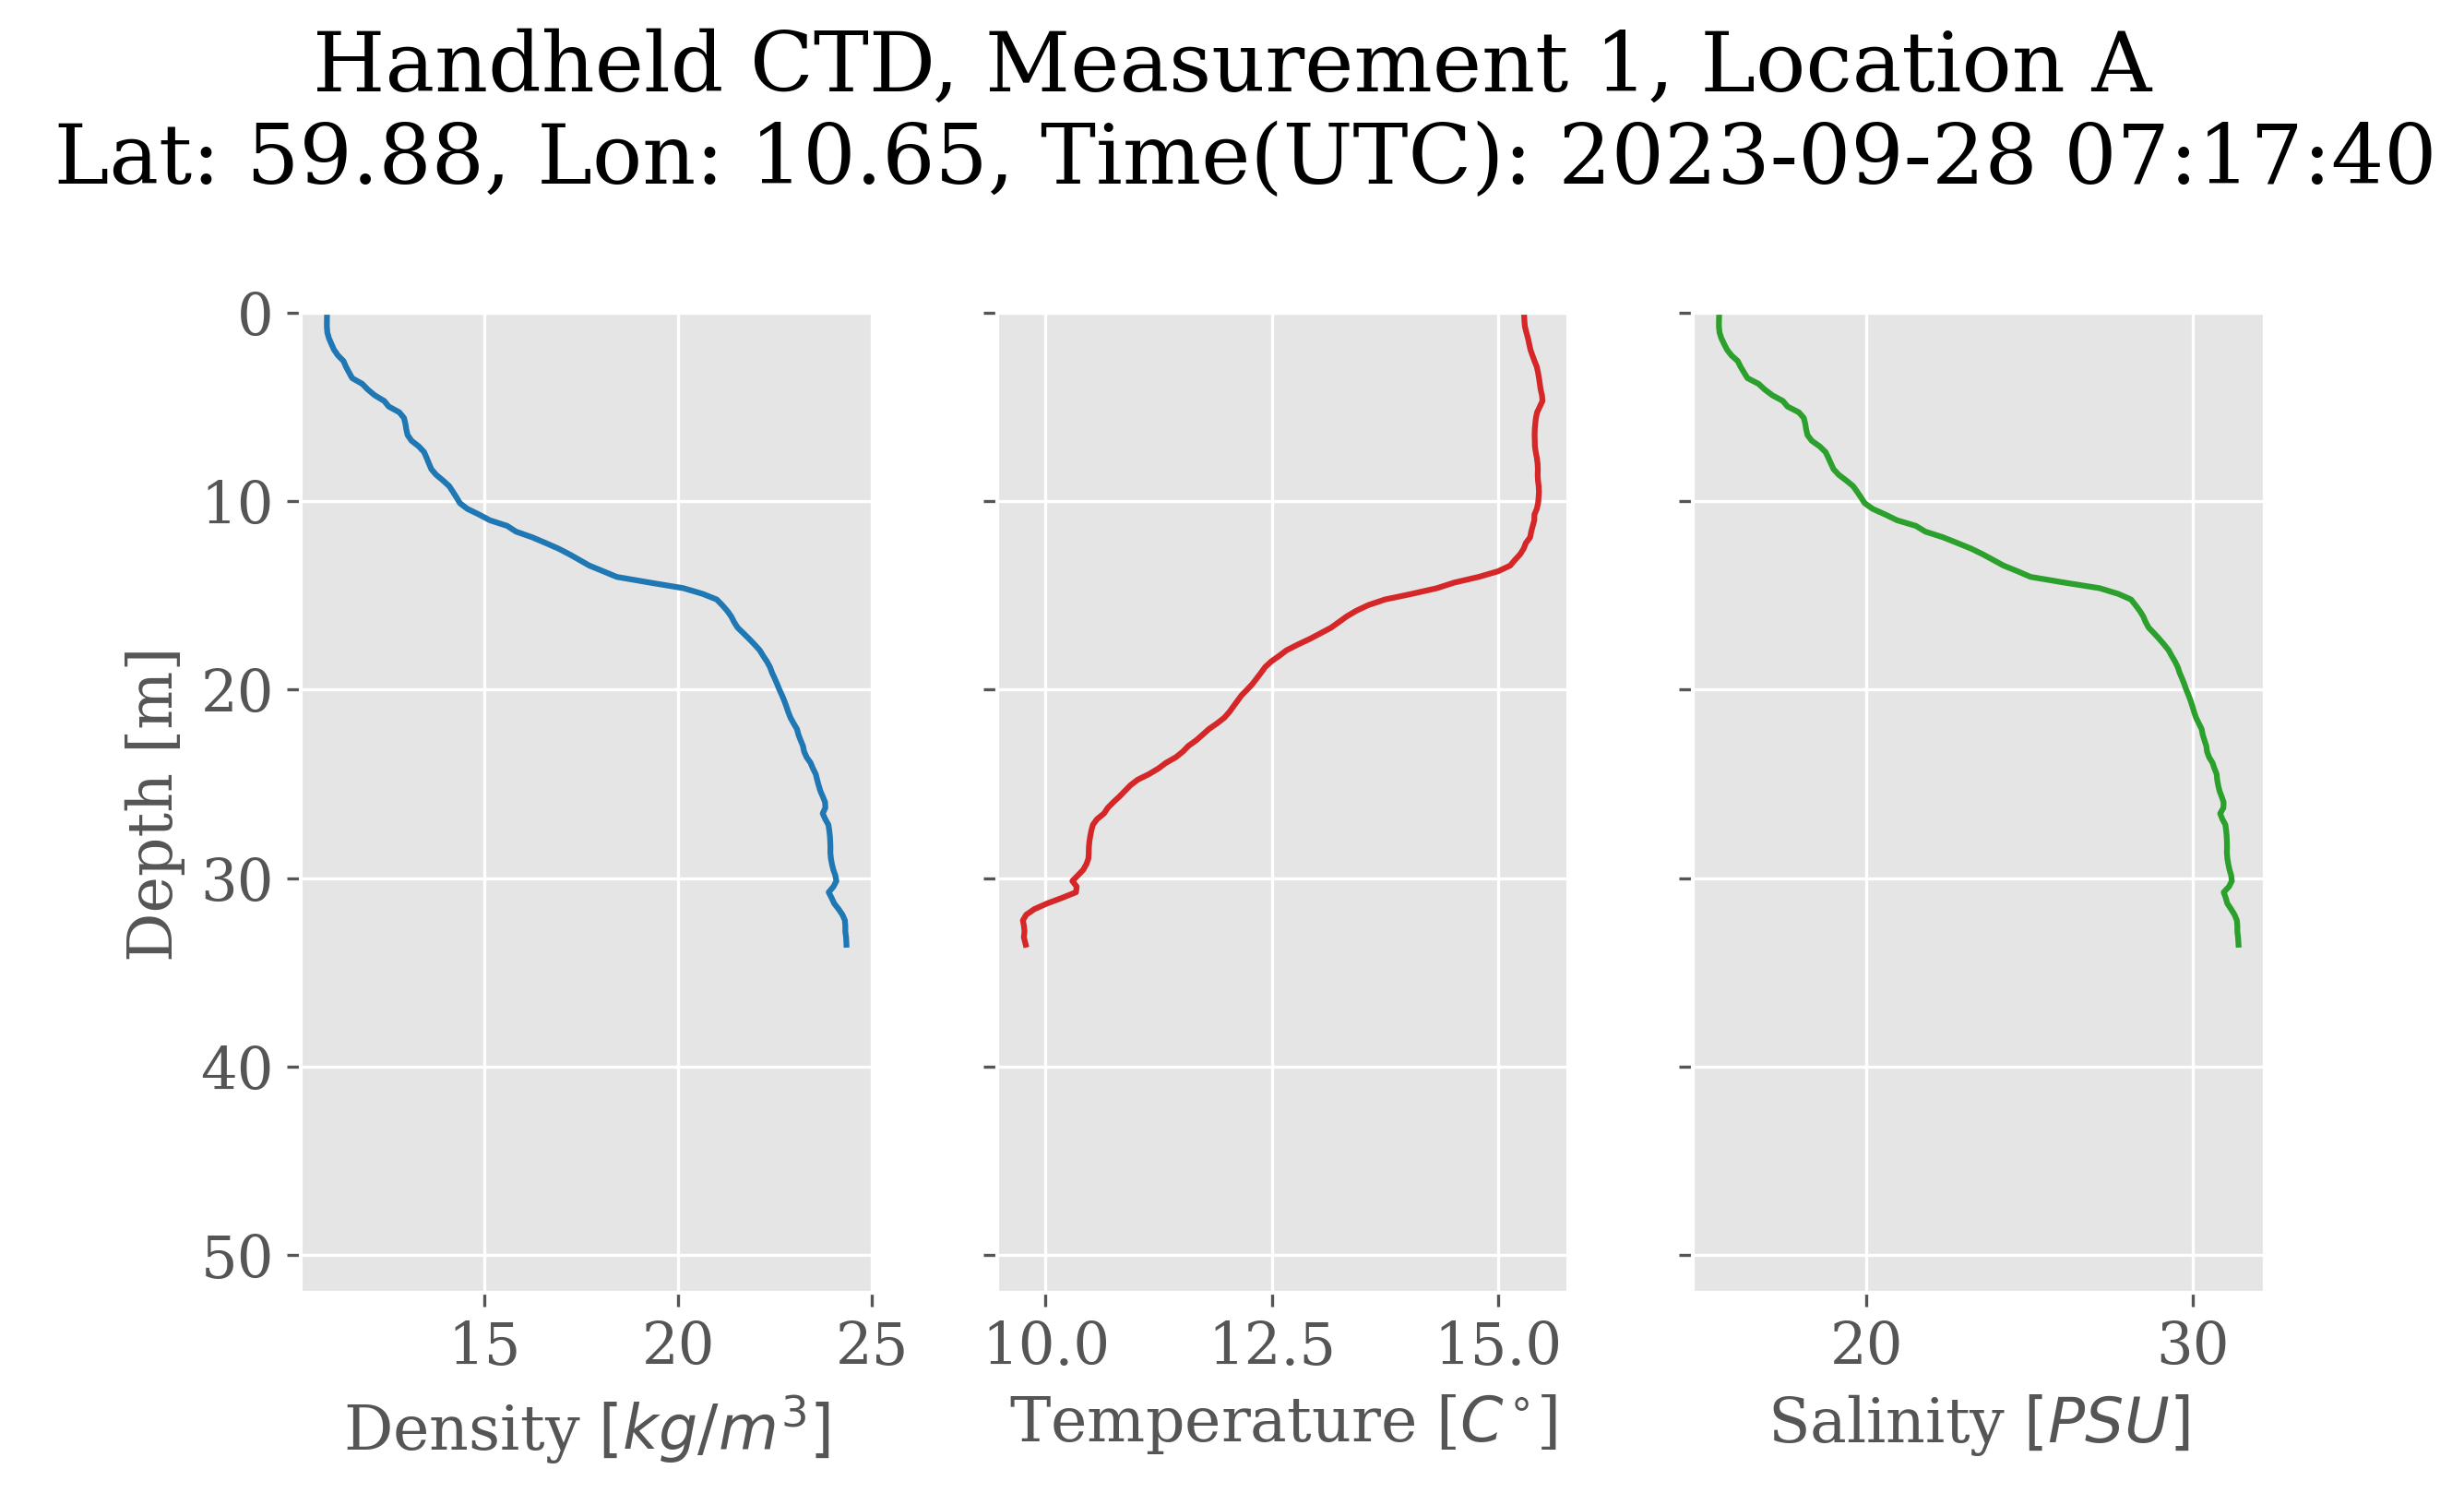
\includegraphics[width=1.\linewidth]{../figures/handheld_ctd/handhedld_ctd_Measurement_1_Location_A.png}
            \caption{}
            \label{fig:handheld_m1lA}
    \end{subfigure}%
    \begin{subfigure}{0.65\textwidth}
            \centering
            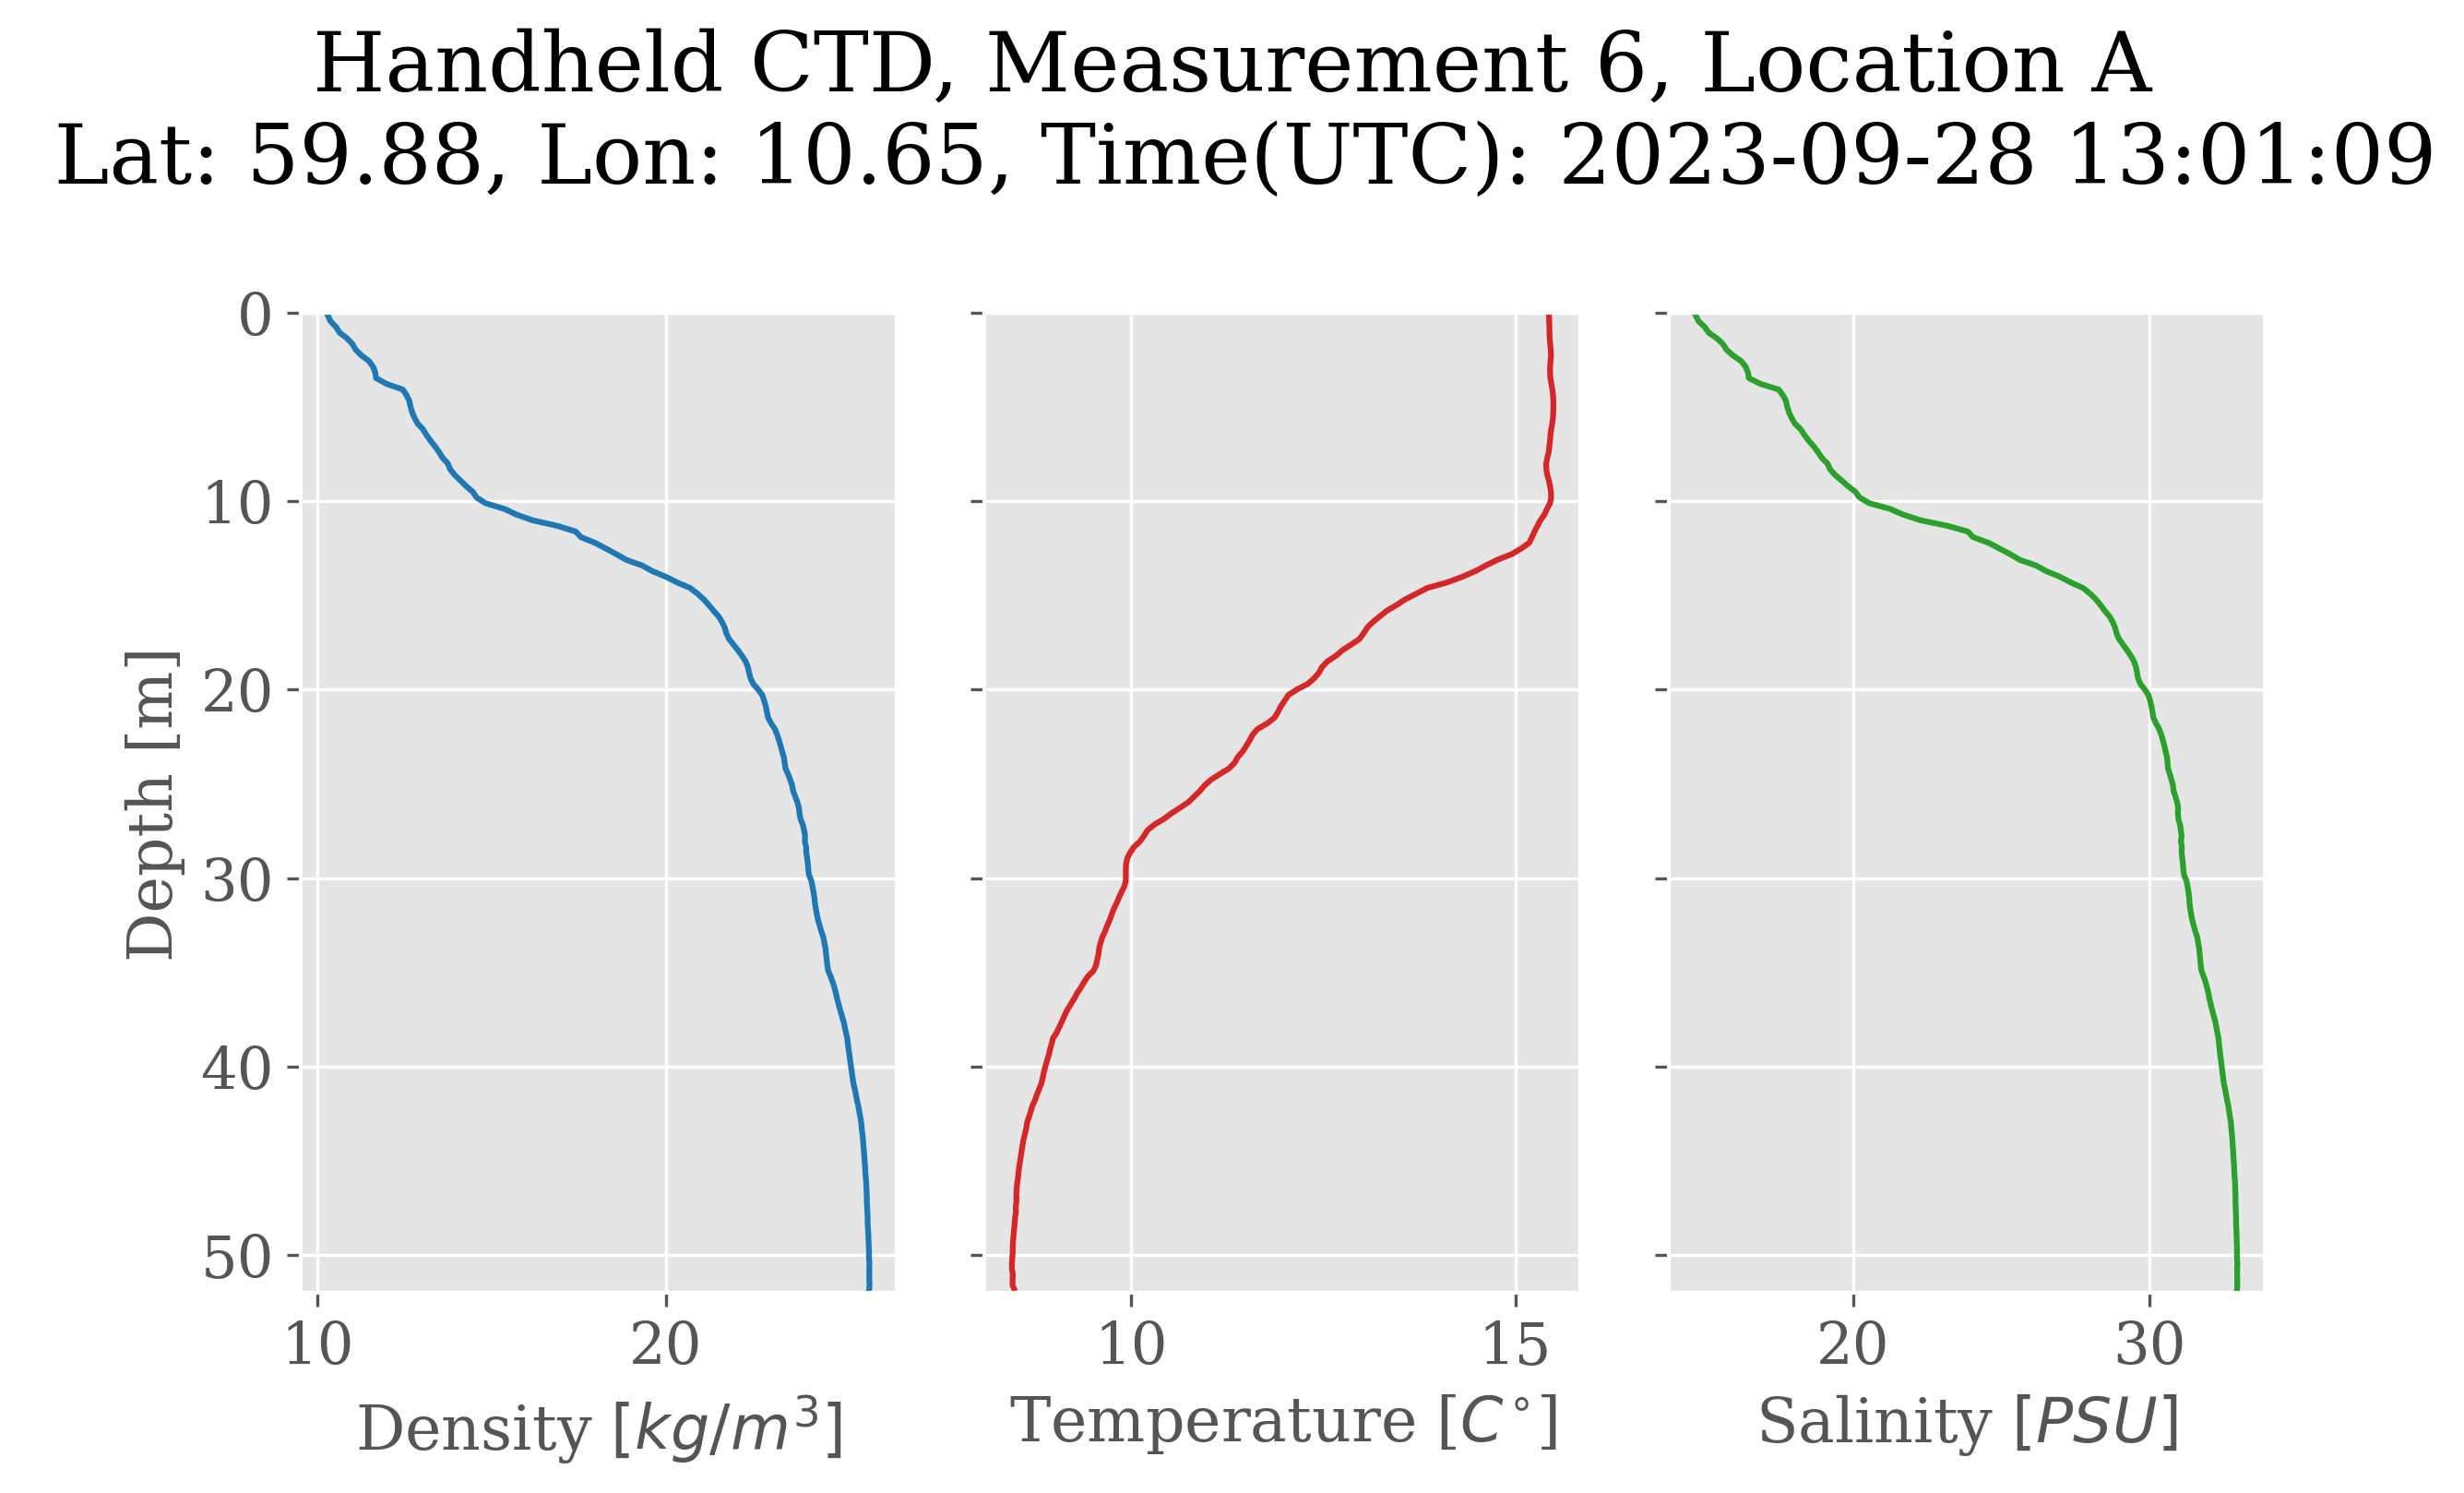
\includegraphics[width=1.\linewidth]{../figures/handheld_ctd/handhedld_ctd_Measurement_6_Location_A.png}
            \caption{}
            \label{fig:handheld_m6lA}
    \end{subfigure}
    
    \begin{subfigure}{0.65\textwidth}
            \centering
            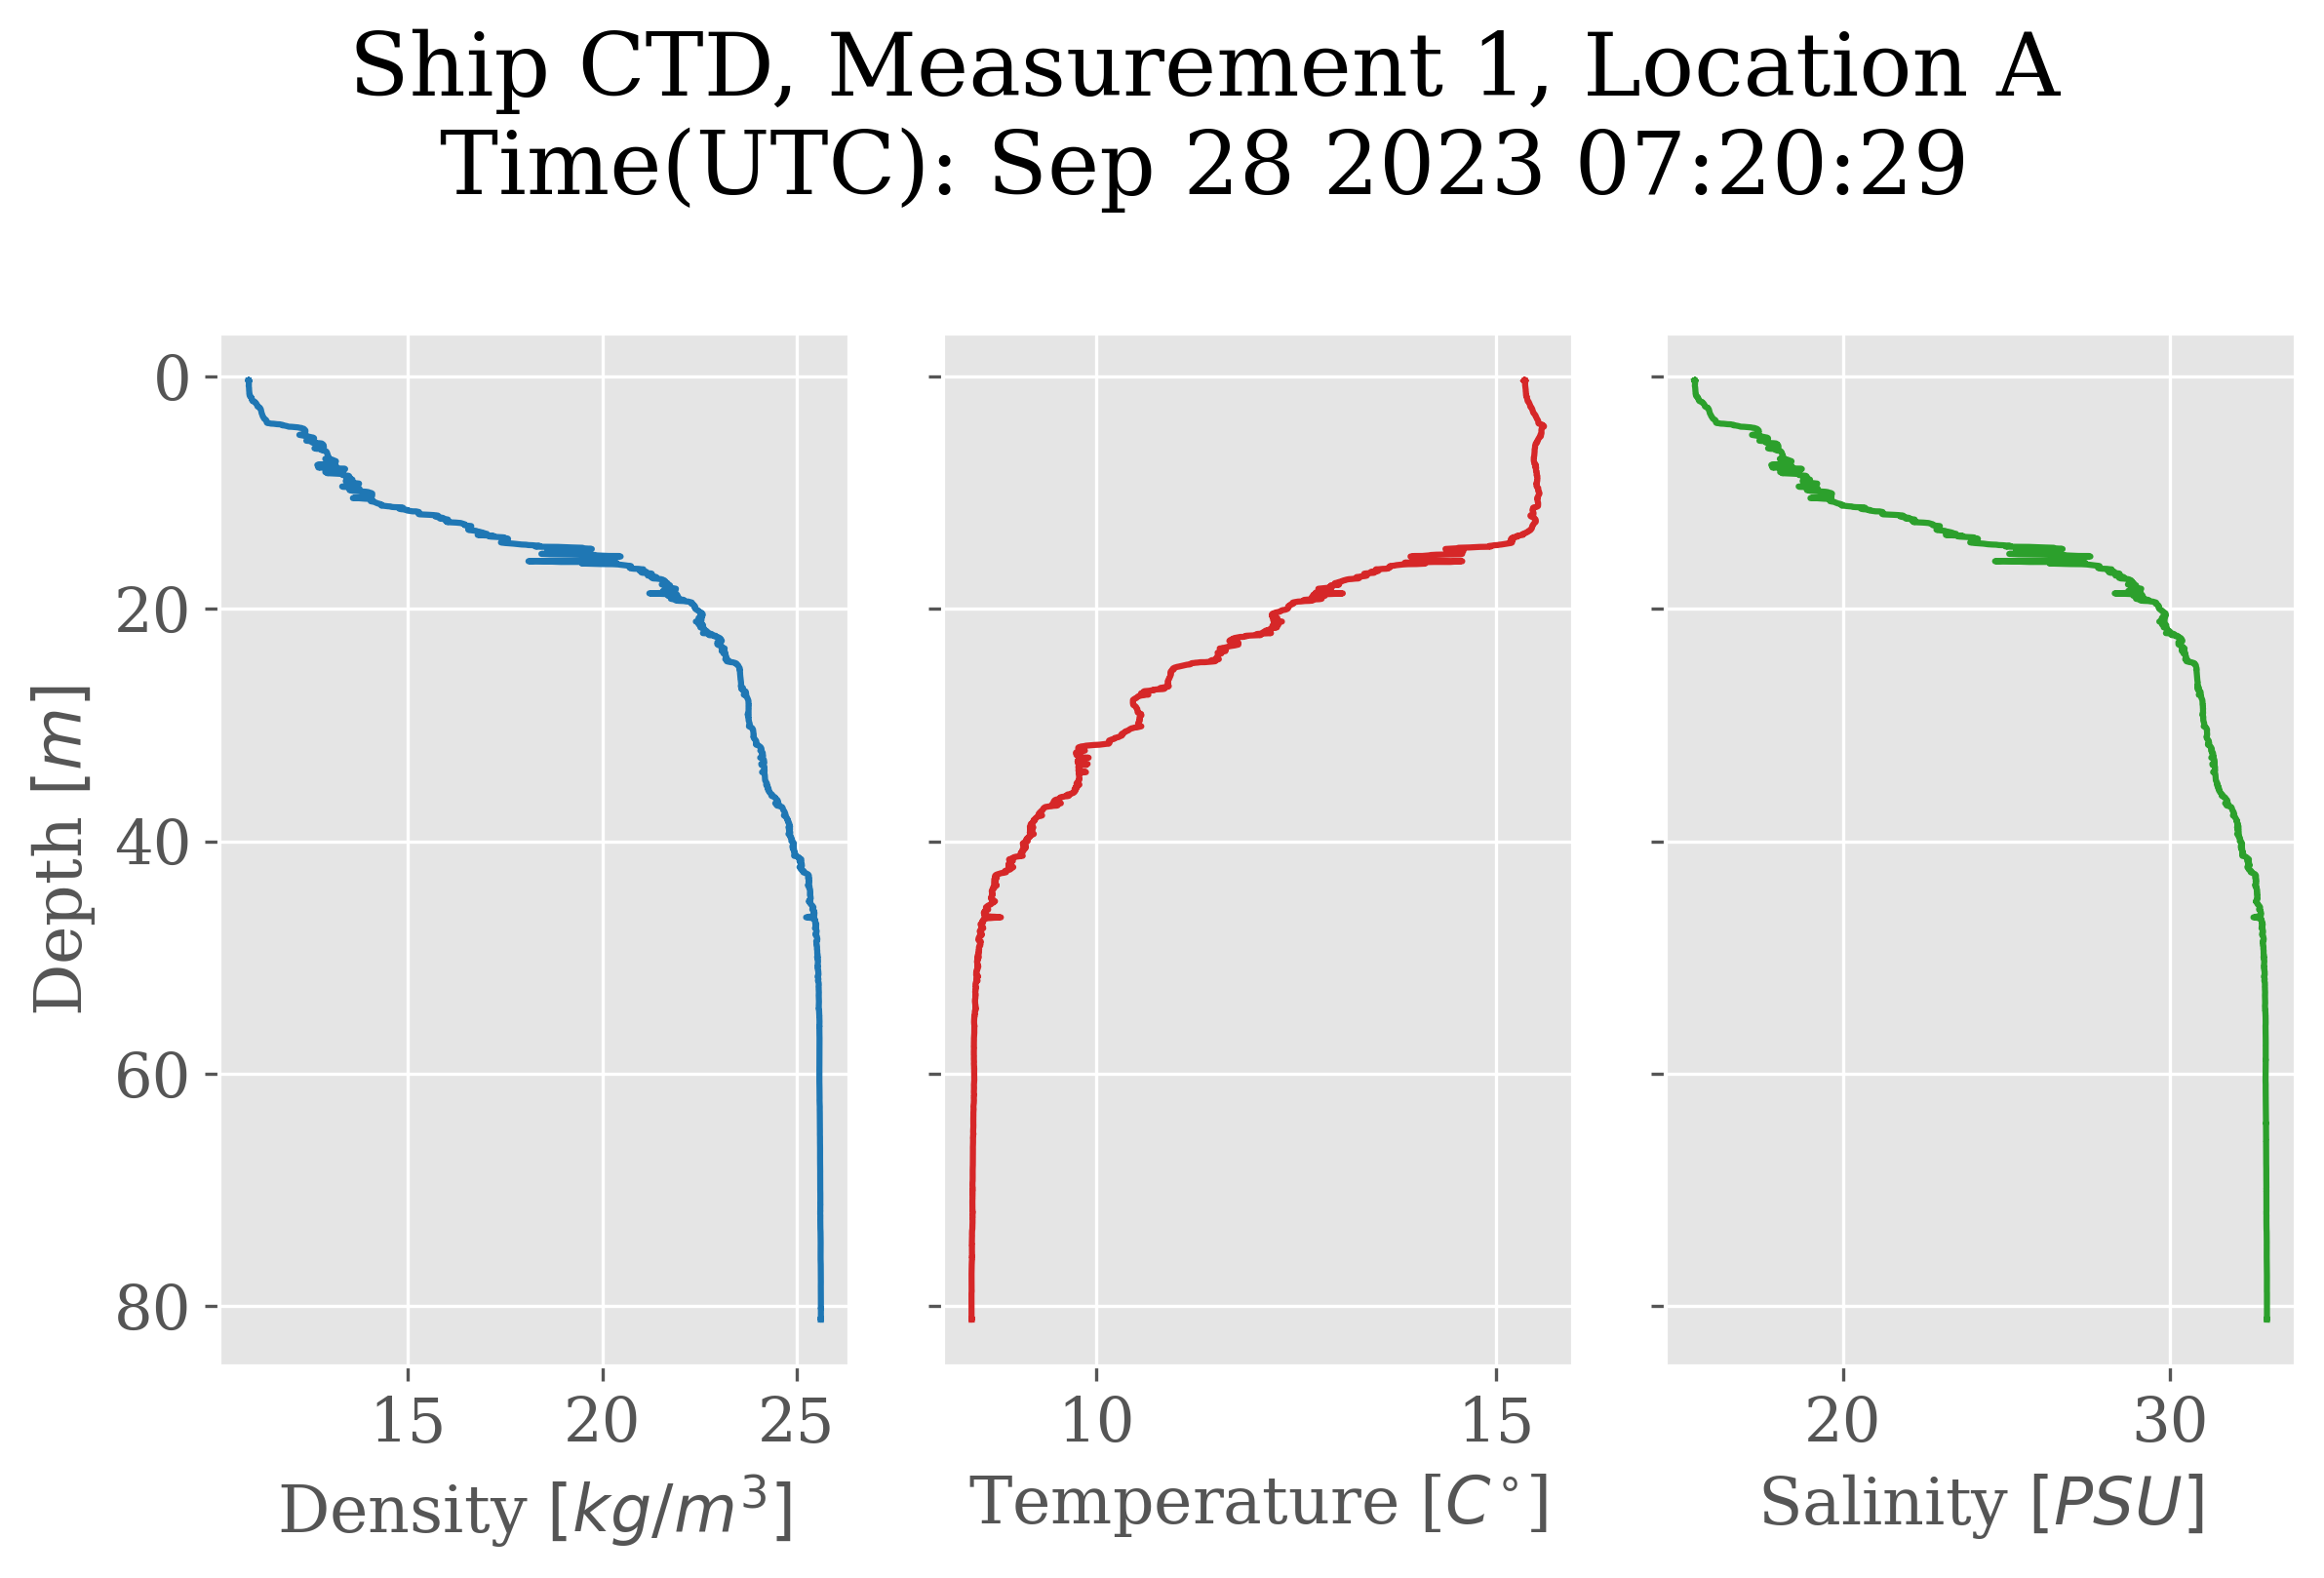
\includegraphics[width=.9\linewidth]{../figures/ship_ctd/ship_ctd_Measurement_1_Location_A.png}
            \caption{}
            \label{fig:ship_m1lA}
    \end{subfigure}%
    \begin{subfigure}{0.65\textwidth}
            \centering
            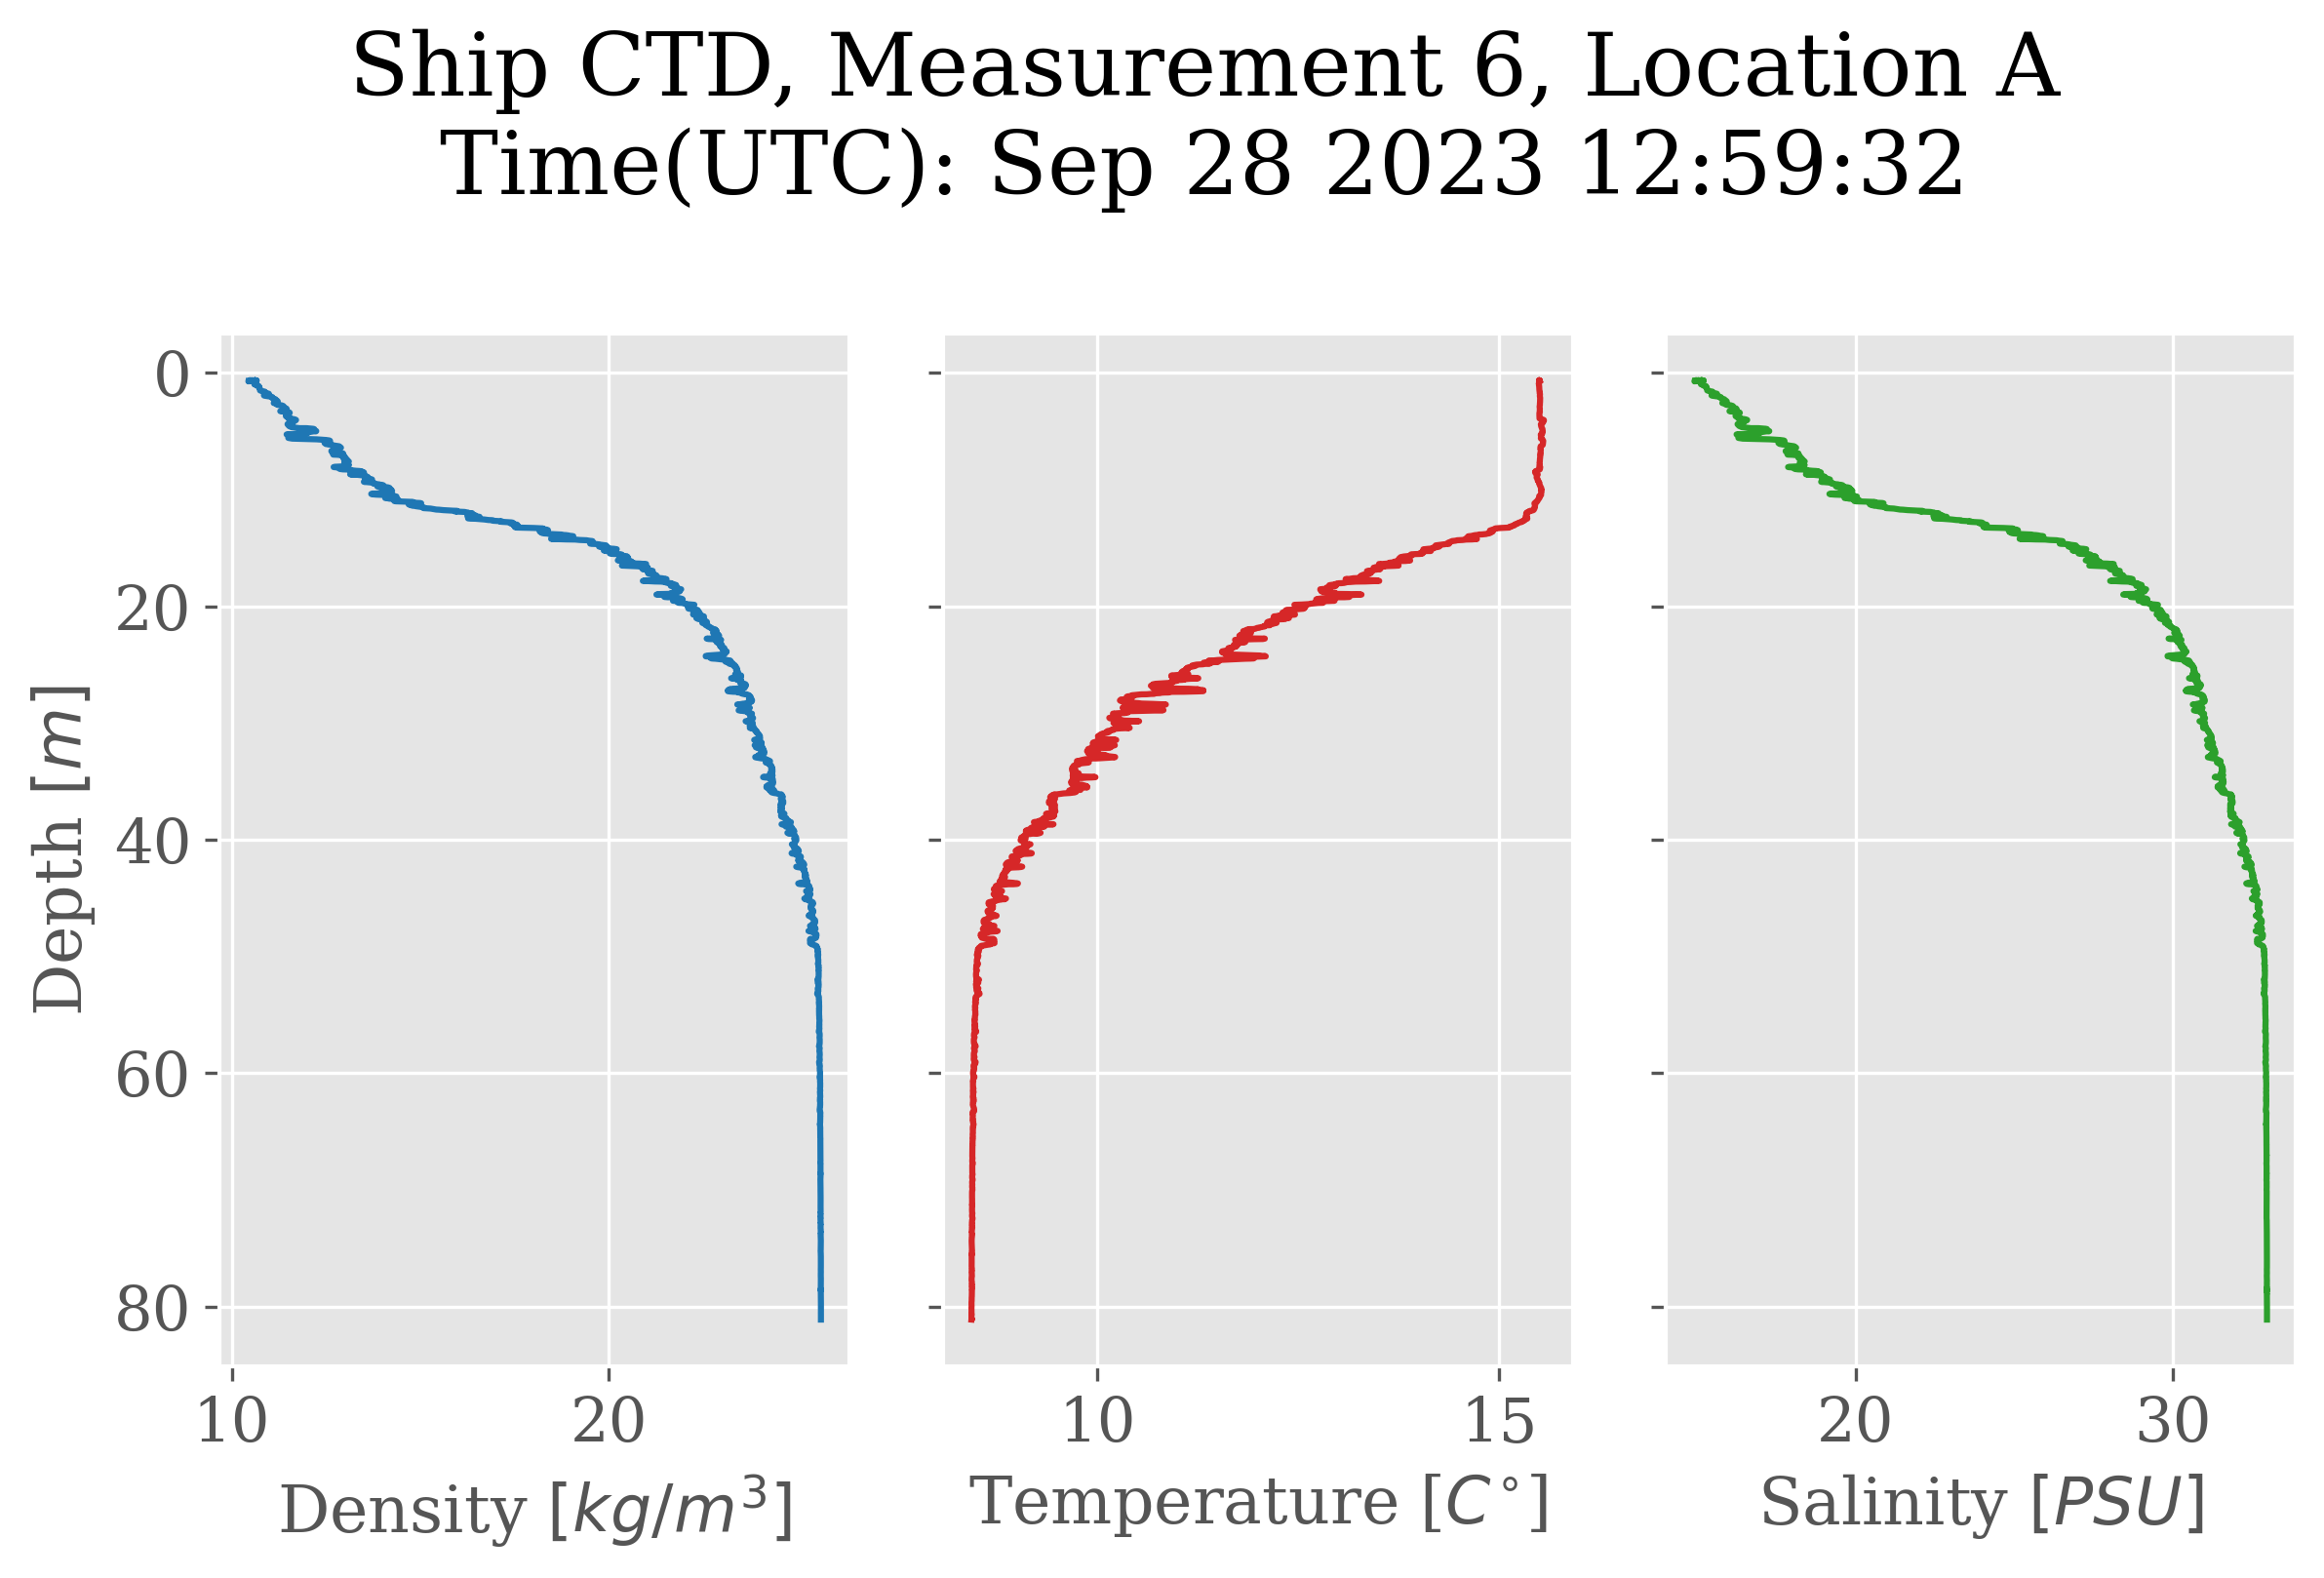
\includegraphics[width=.9\linewidth]{../figures/ship_ctd/ship_ctd_Measurement_6_Location_A.png}
            \caption{}
            \label{fig:ship_m6lA}
    \end{subfigure}
    \end{adjustwidth}
    
    \caption{Handheld (above) and ship (below) CTD measurements at location A. Each shows a depth profile of density, temperature and salinity.}
    \label{fig:location_Aapp}
    \end{figure}
    
    % station B
    \begin{figure}[H]
        \begin{adjustwidth}{-2.5cm}{-2.5cm}  % Adjust the values to change the margins
        \begin{subfigure}{0.65\textwidth}
                \centering
                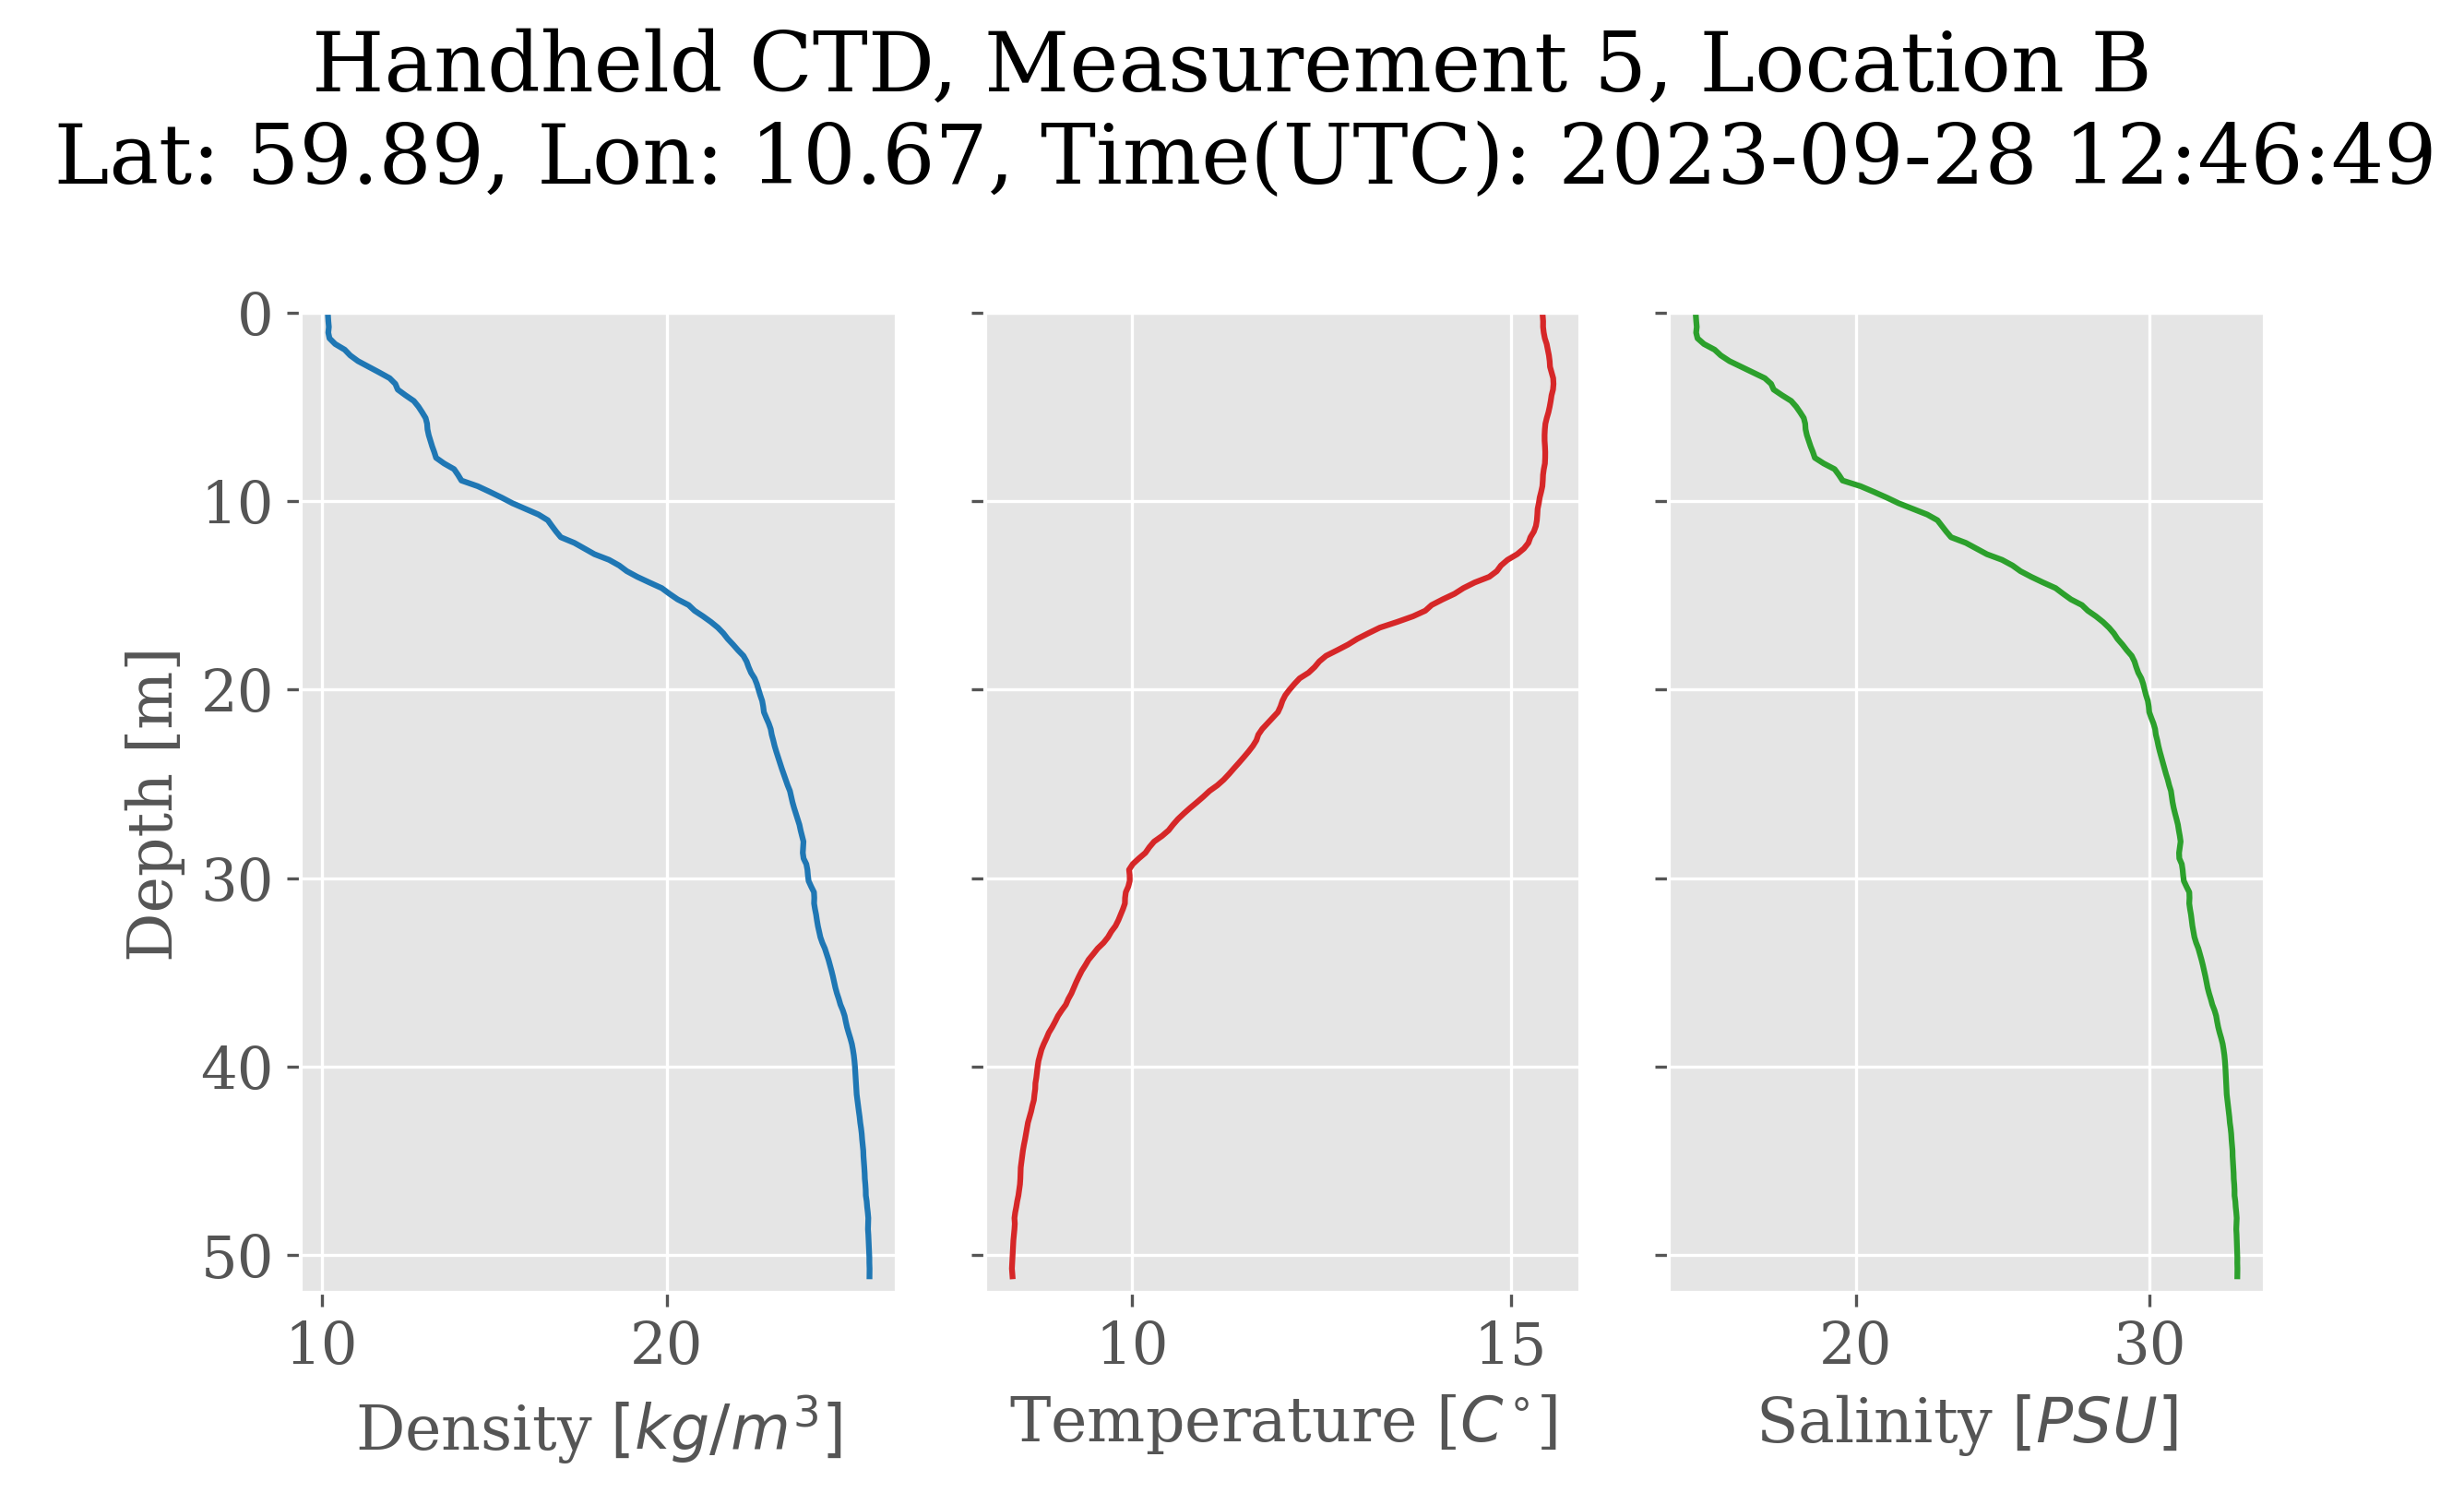
\includegraphics[width=1.\linewidth]{../figures/handheld_ctd/handhedld_ctd_Measurement_5_Location_B.png}
                \caption{}
                \label{fig:handheld_m1lA}
        \end{subfigure}%
        \begin{subfigure}{0.65\textwidth}
                \centering
                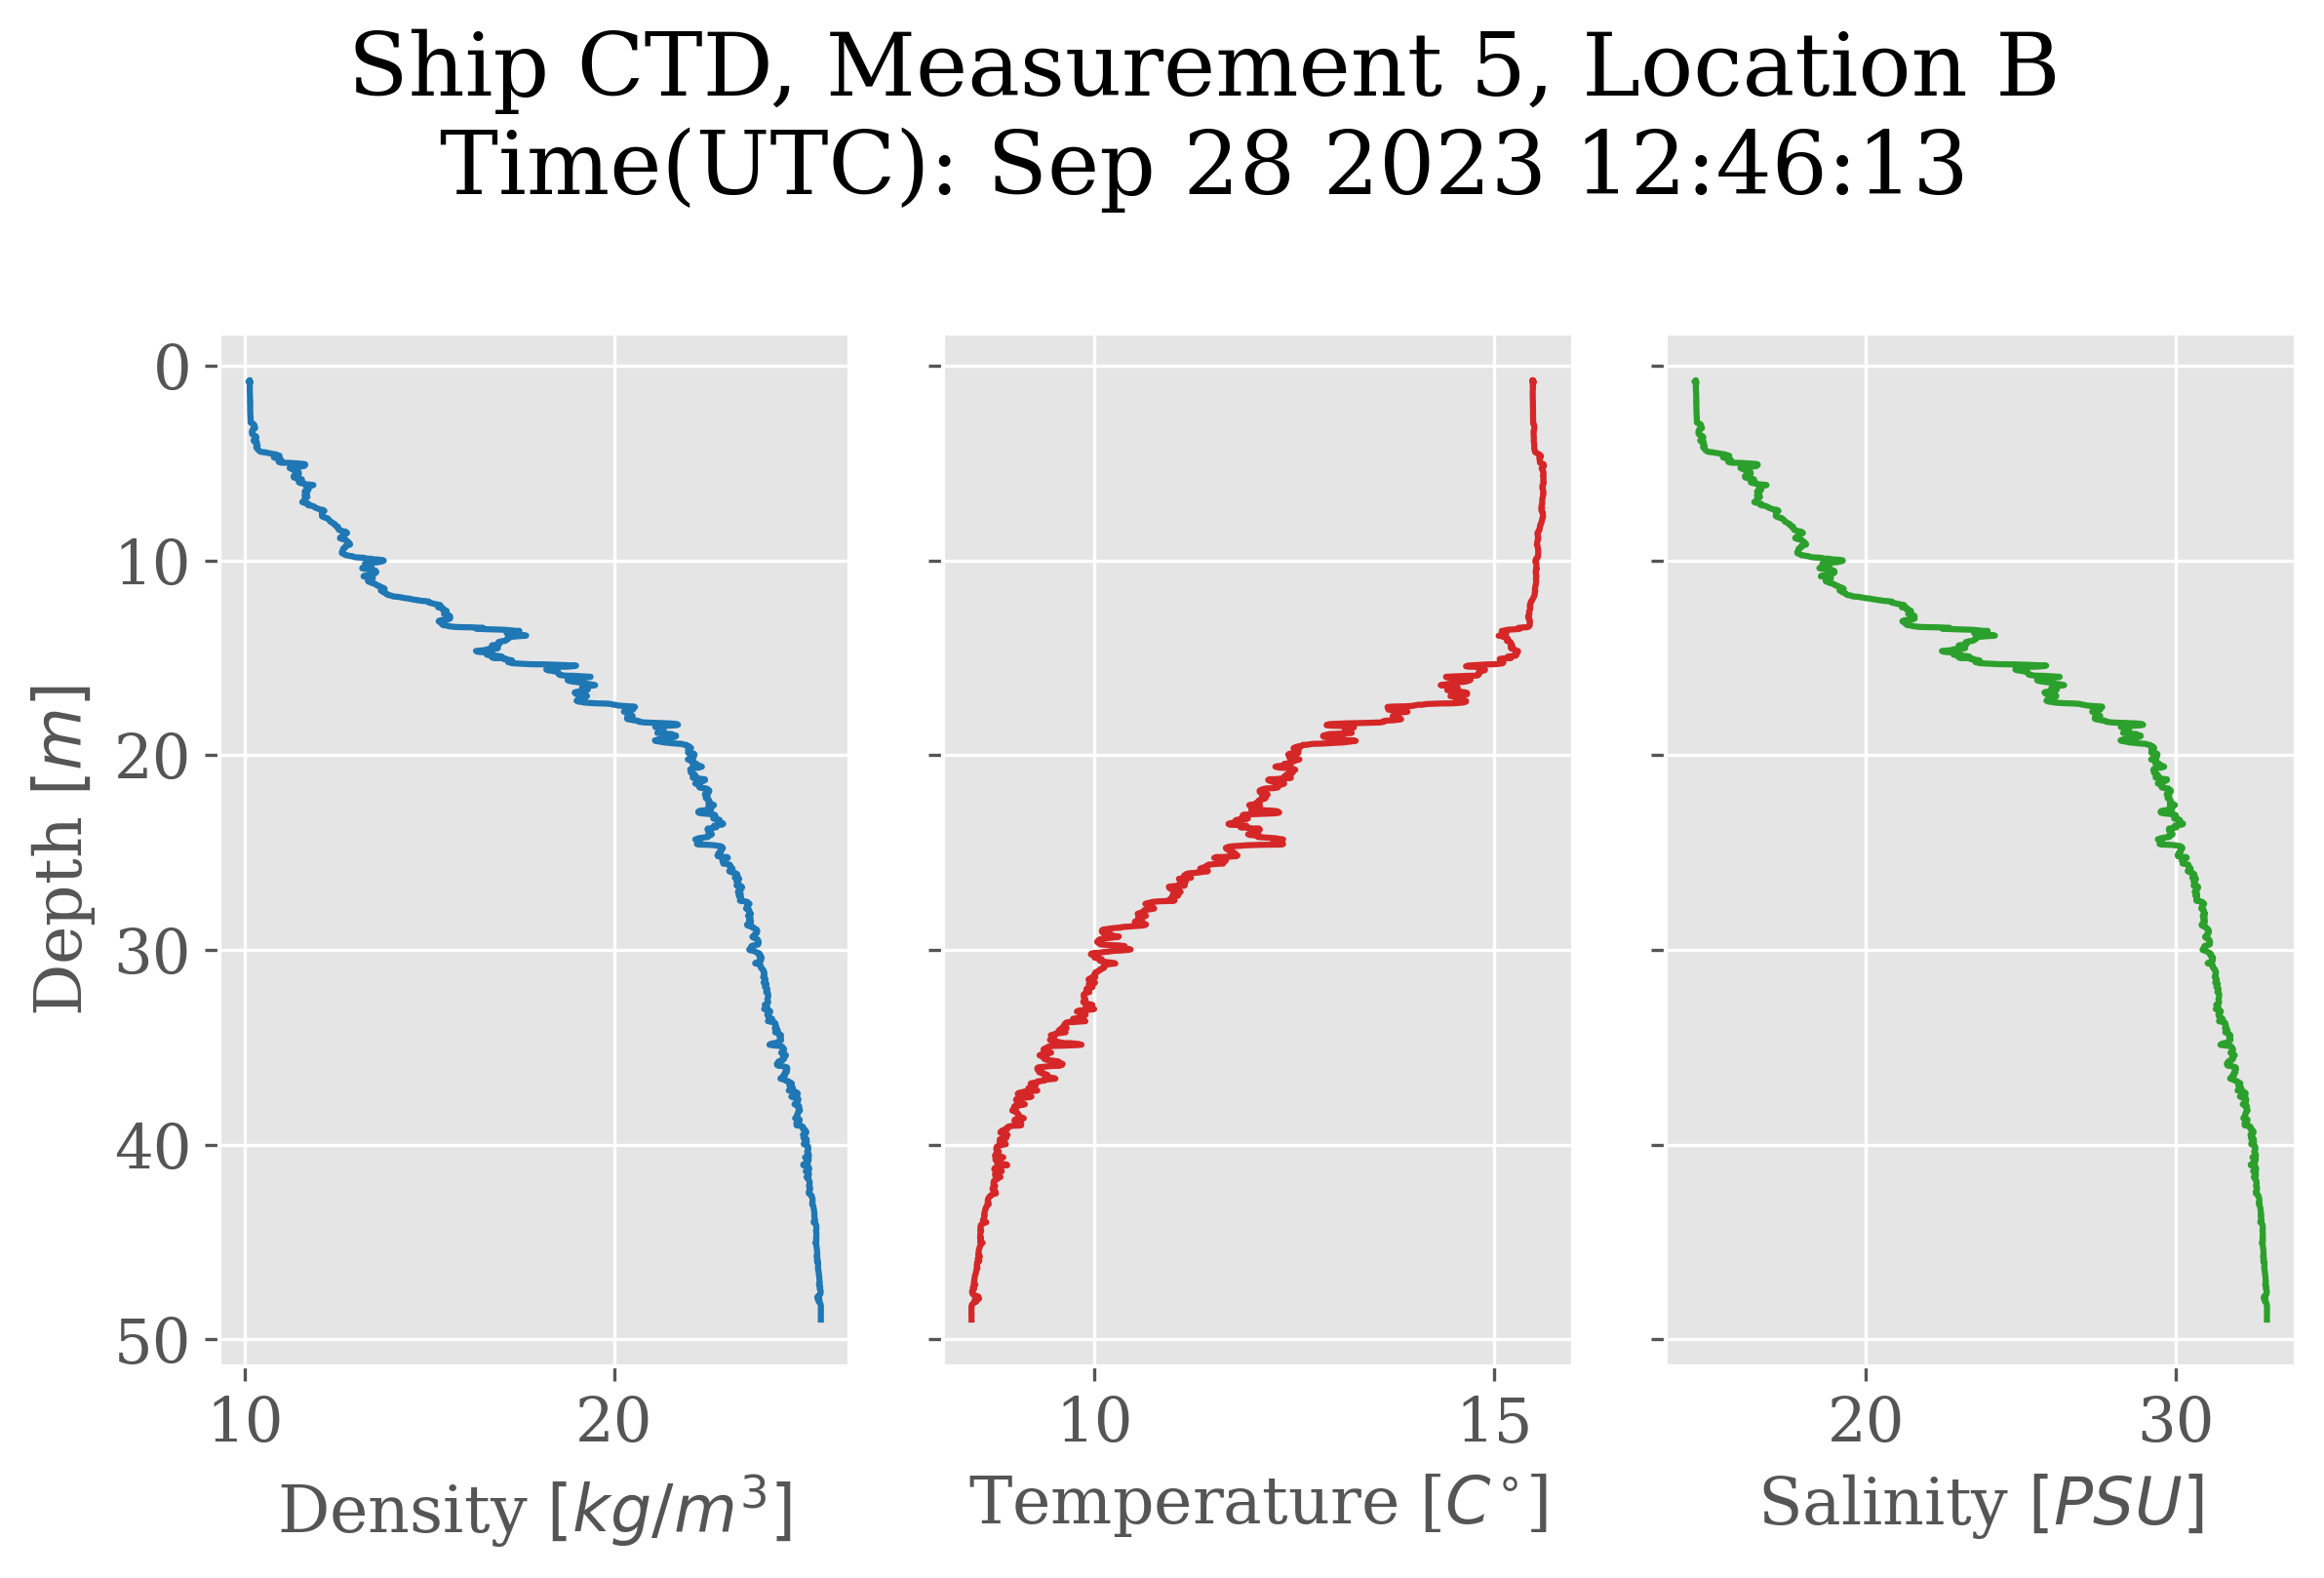
\includegraphics[width=1.\linewidth]{../figures/ship_ctd/ship_ctd_Measurement_5_Location_B.png}
                \caption{}
                \label{fig:handheld_m6lA}
        \end{subfigure}
        \end{adjustwidth}
        
        \caption{Handheld (left) and ship (right) CTD measurements at location A. Each shows a depth profile of density, temperature and salinity.}
        \label{fig:location_Aapp}
        \end{figure}
    
    %station C
    \begin{figure}[H]
            \begin{adjustwidth}{-2.5cm}{-2.5cm}  % Adjust the values to change the margins
            \begin{subfigure}{0.65\textwidth}
                \centering
                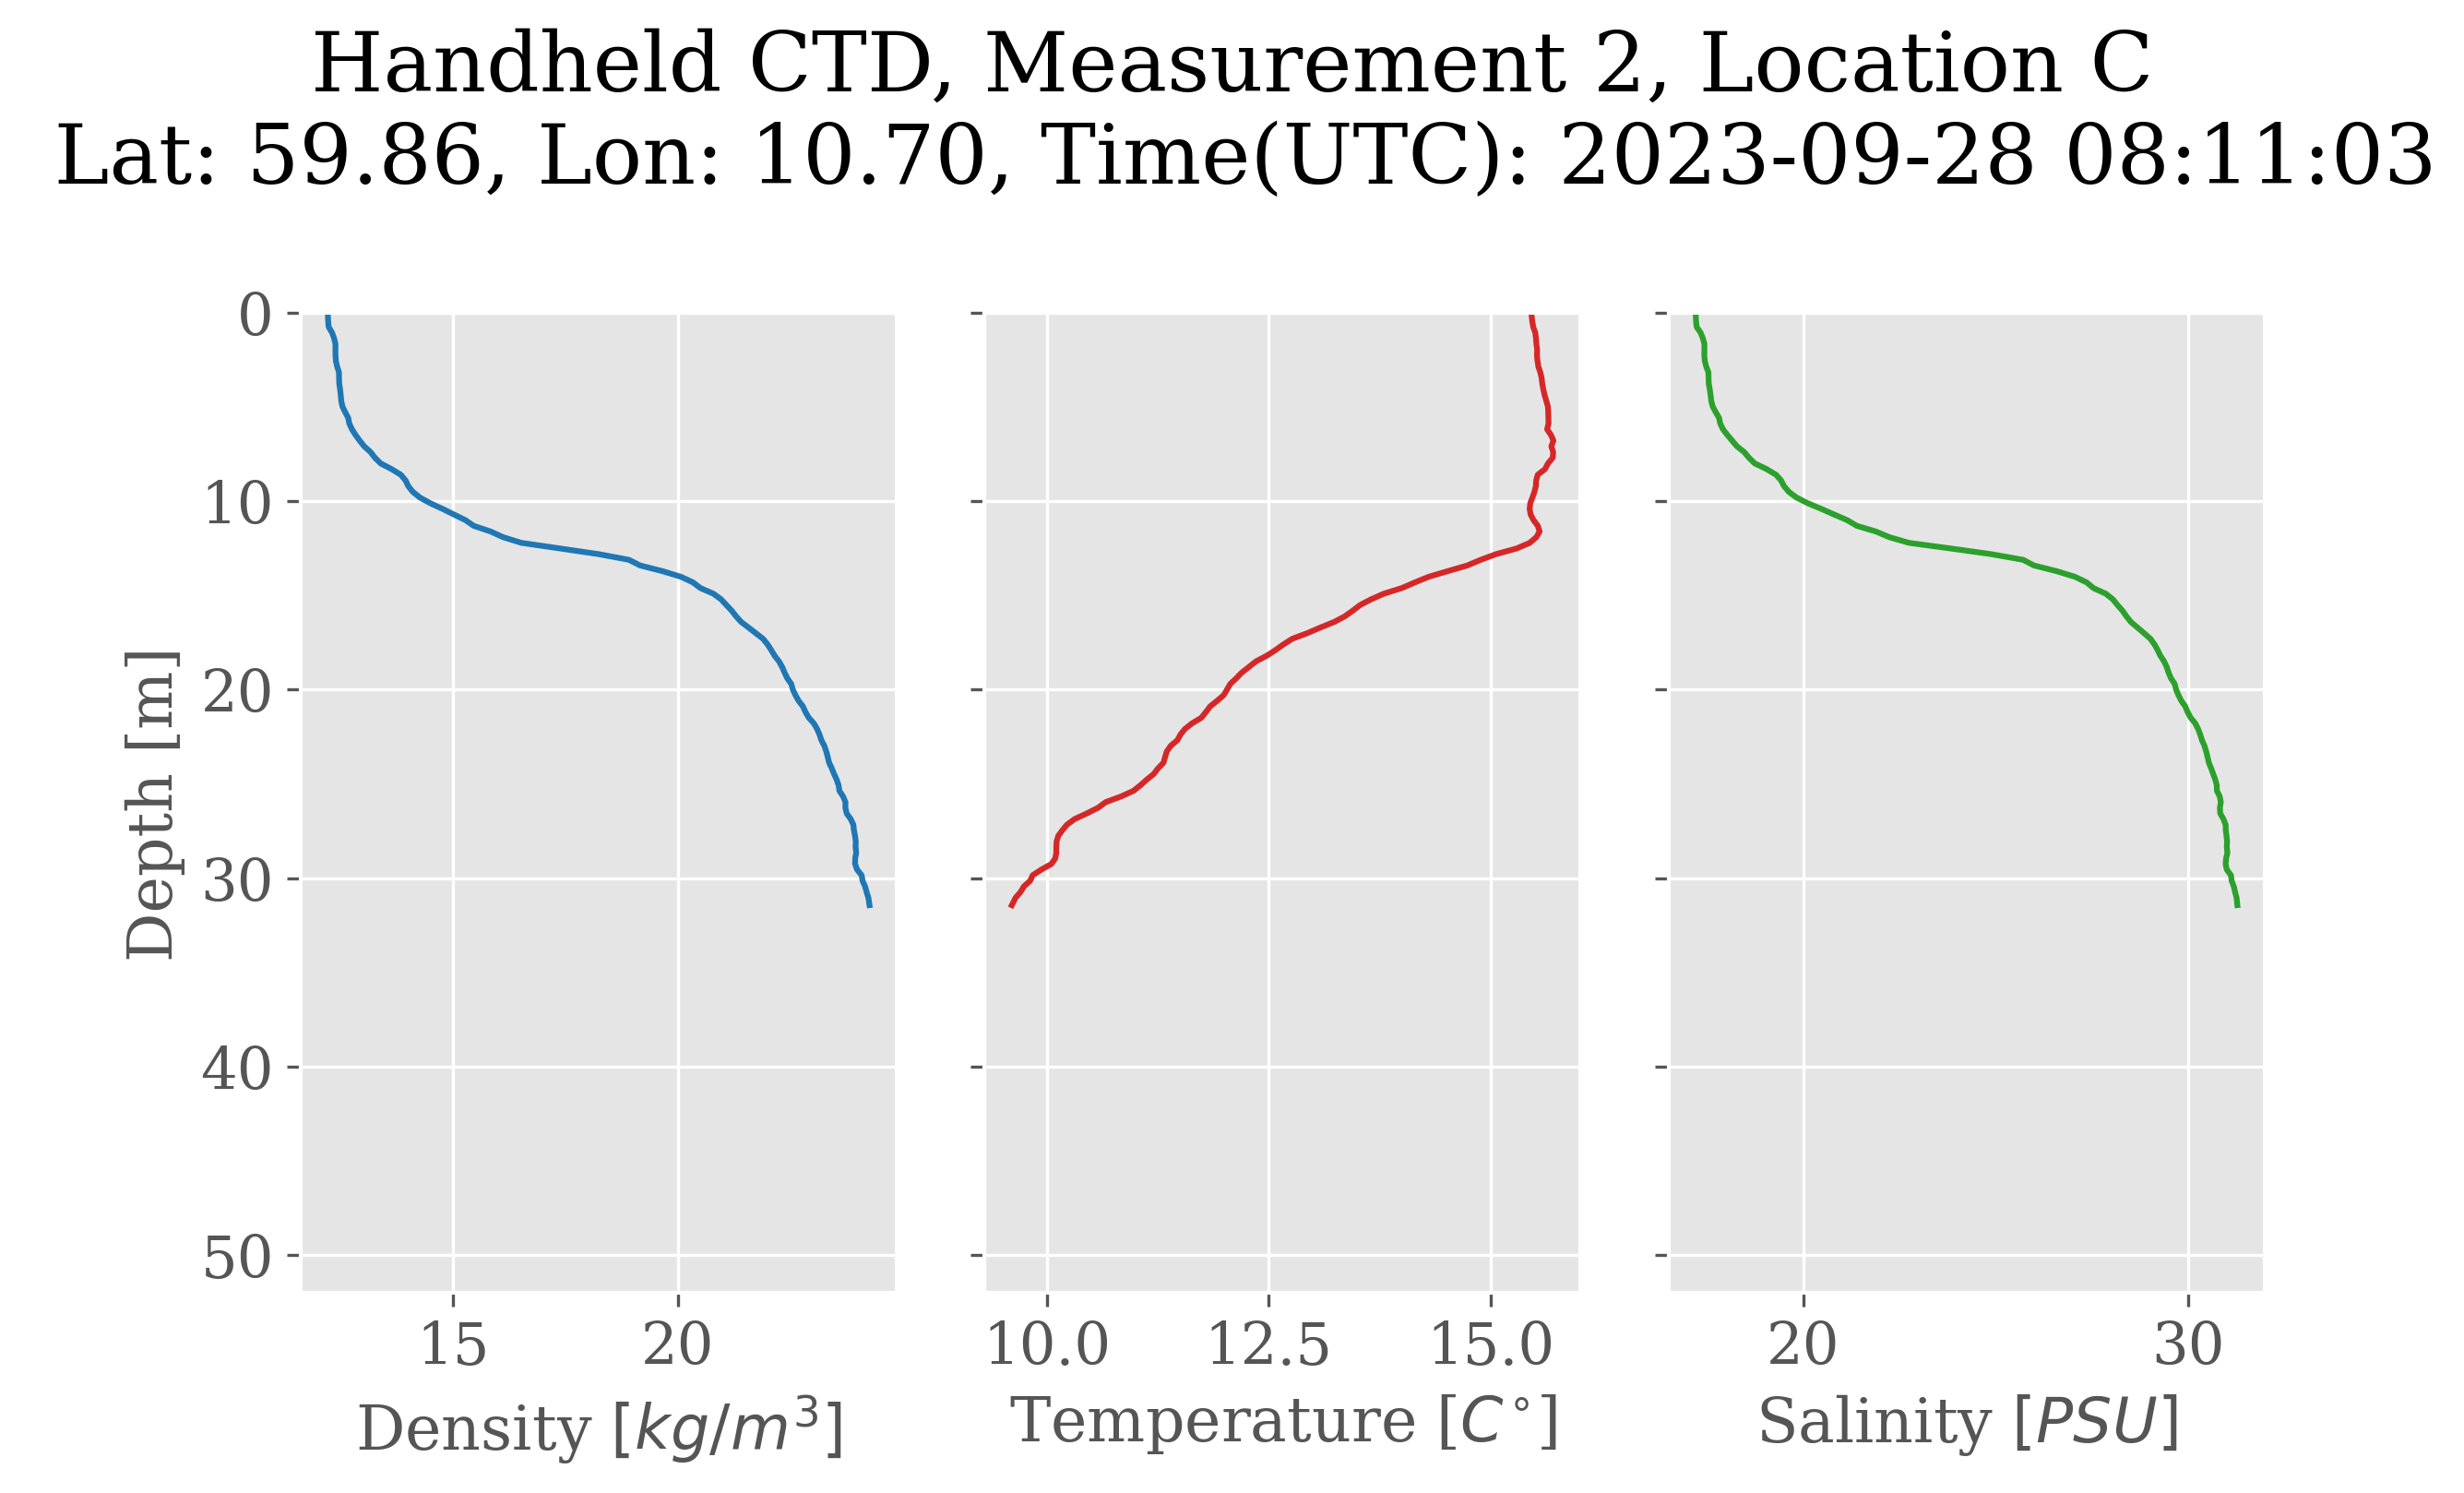
\includegraphics[width=1.\linewidth]{../figures/handheld_ctd/handhedld_ctd_Measurement_2_Location_C.png}
                \caption{}
                \label{fig:handheld_m2lC}
            \end{subfigure}%
            \begin{subfigure}{0.65\textwidth}
                \centering
                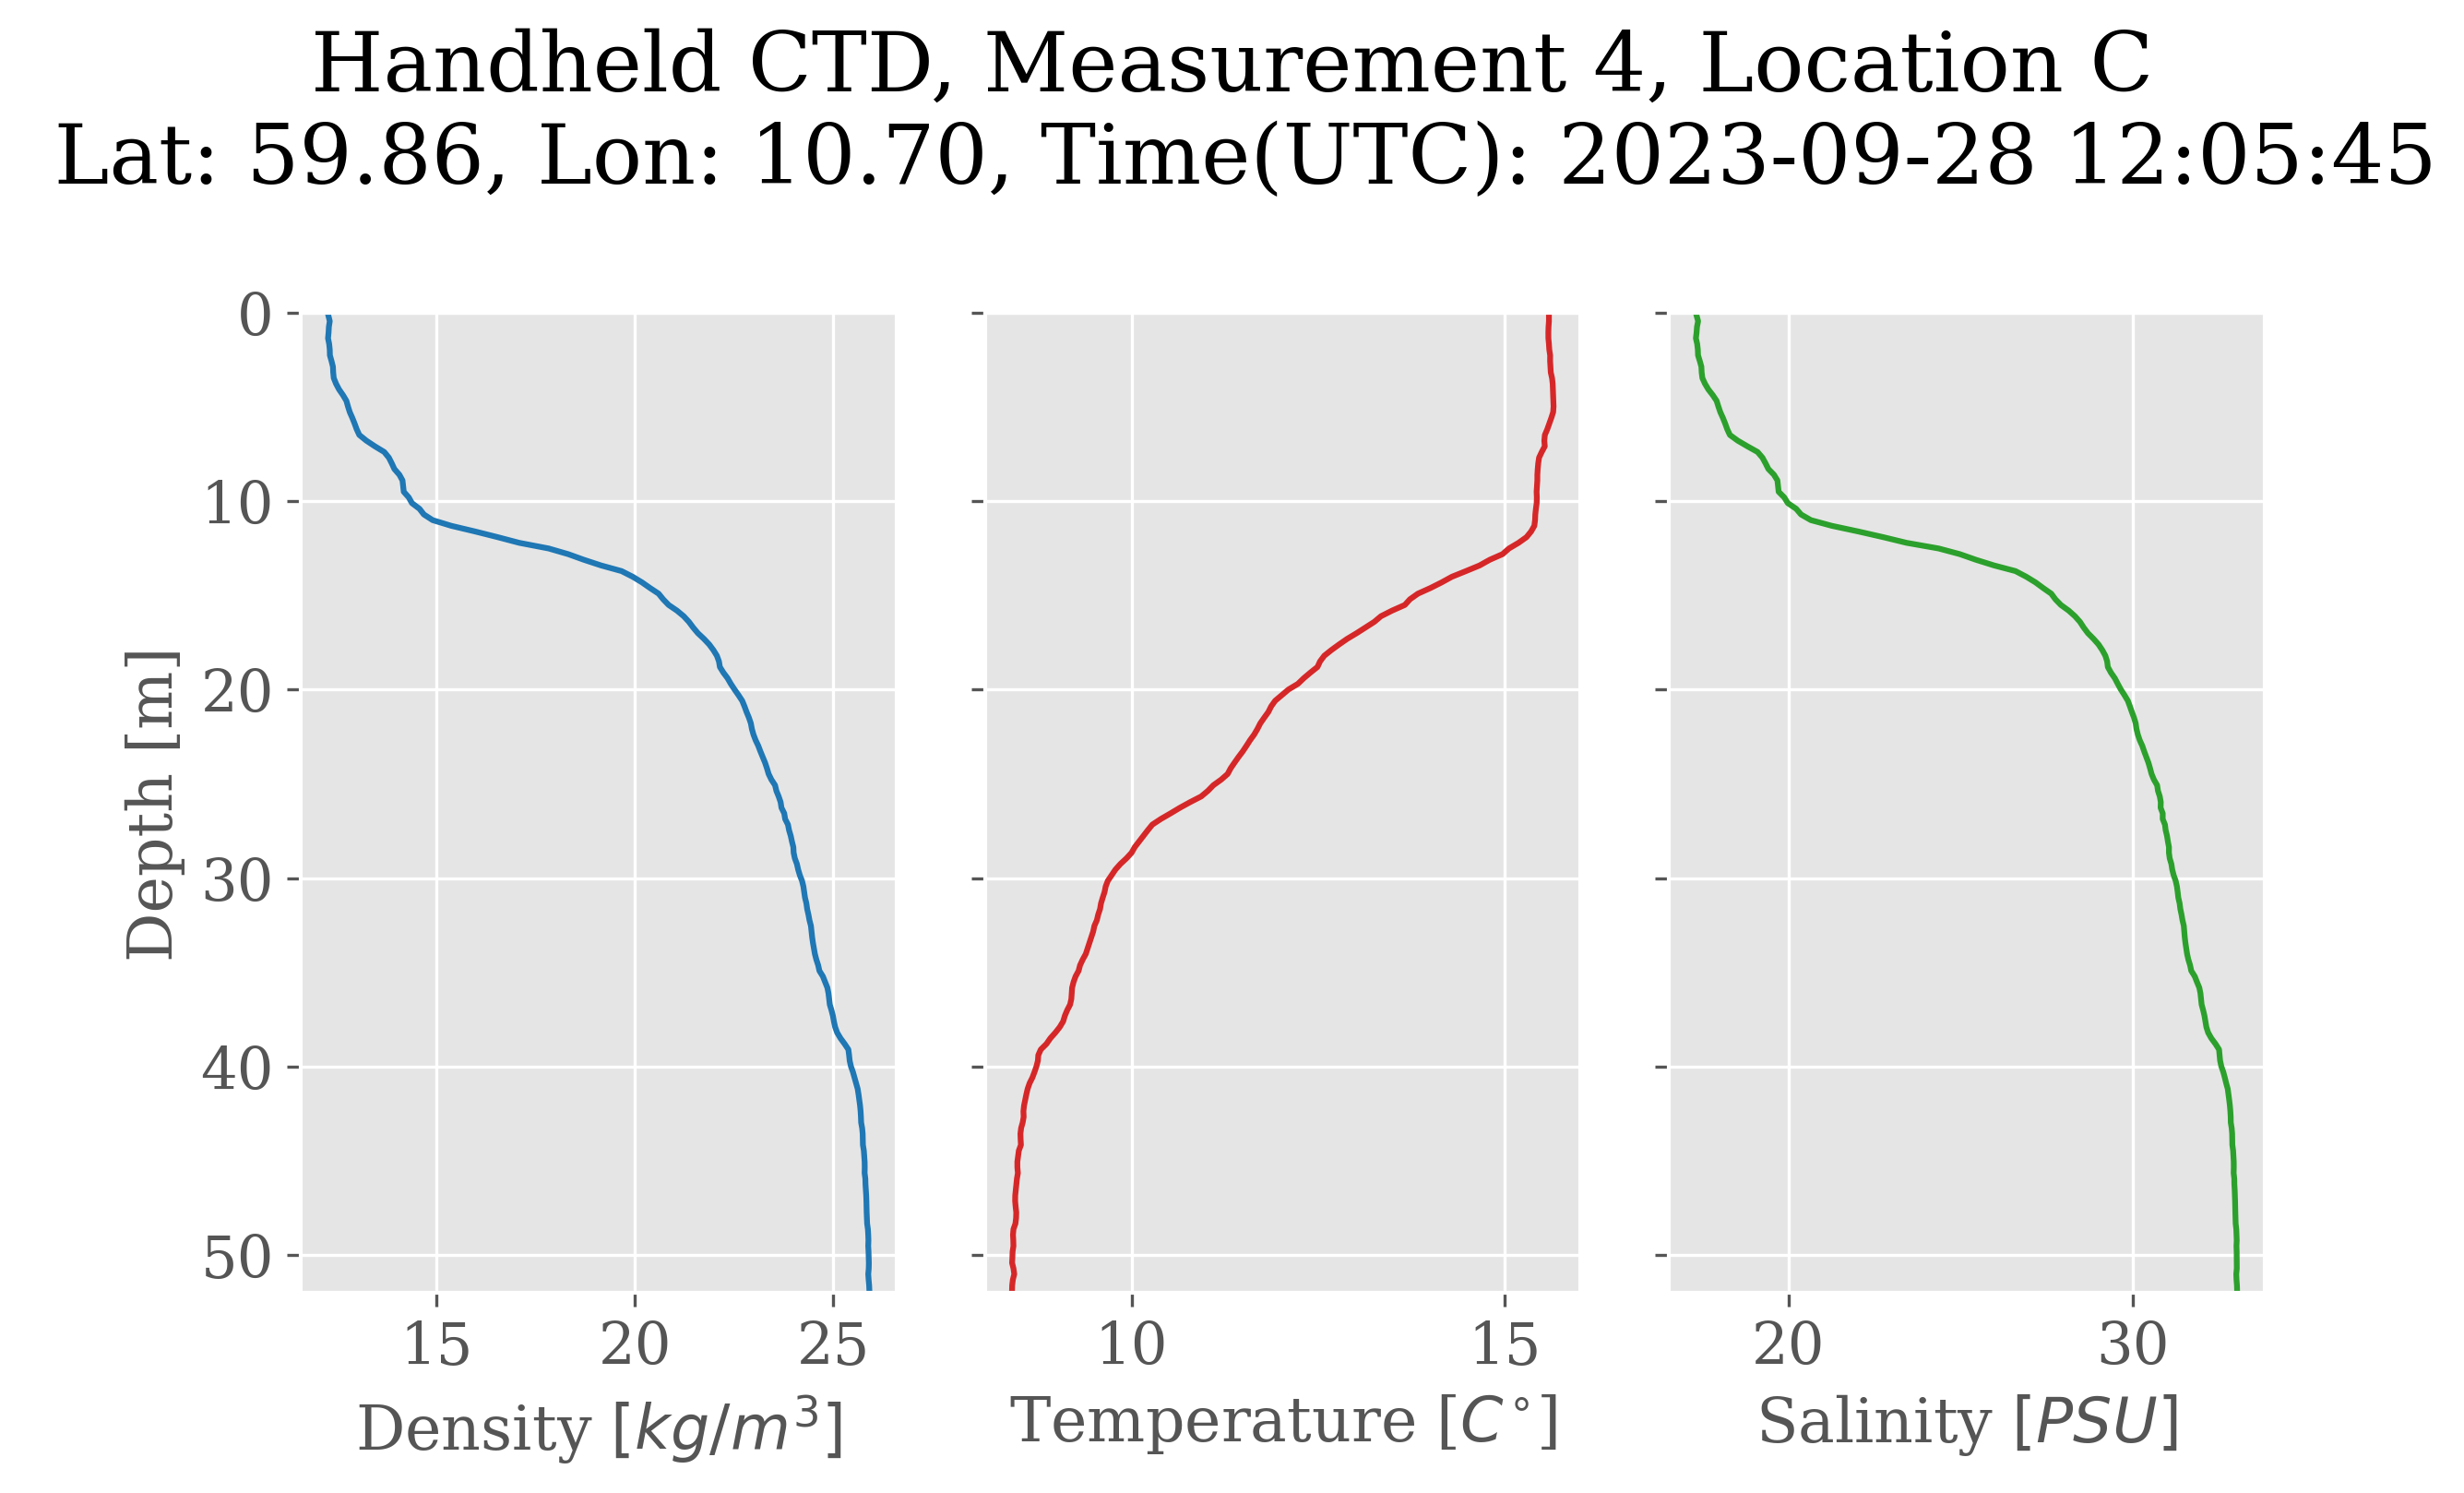
\includegraphics[width=1.\linewidth]{../figures/handheld_ctd/handhedld_ctd_Measurement_4_Location_C.png}
                \caption{}
                \label{fig:handheld_m4lC}
            \end{subfigure}
        
            \begin{subfigure}{0.65\textwidth}
                \centering
                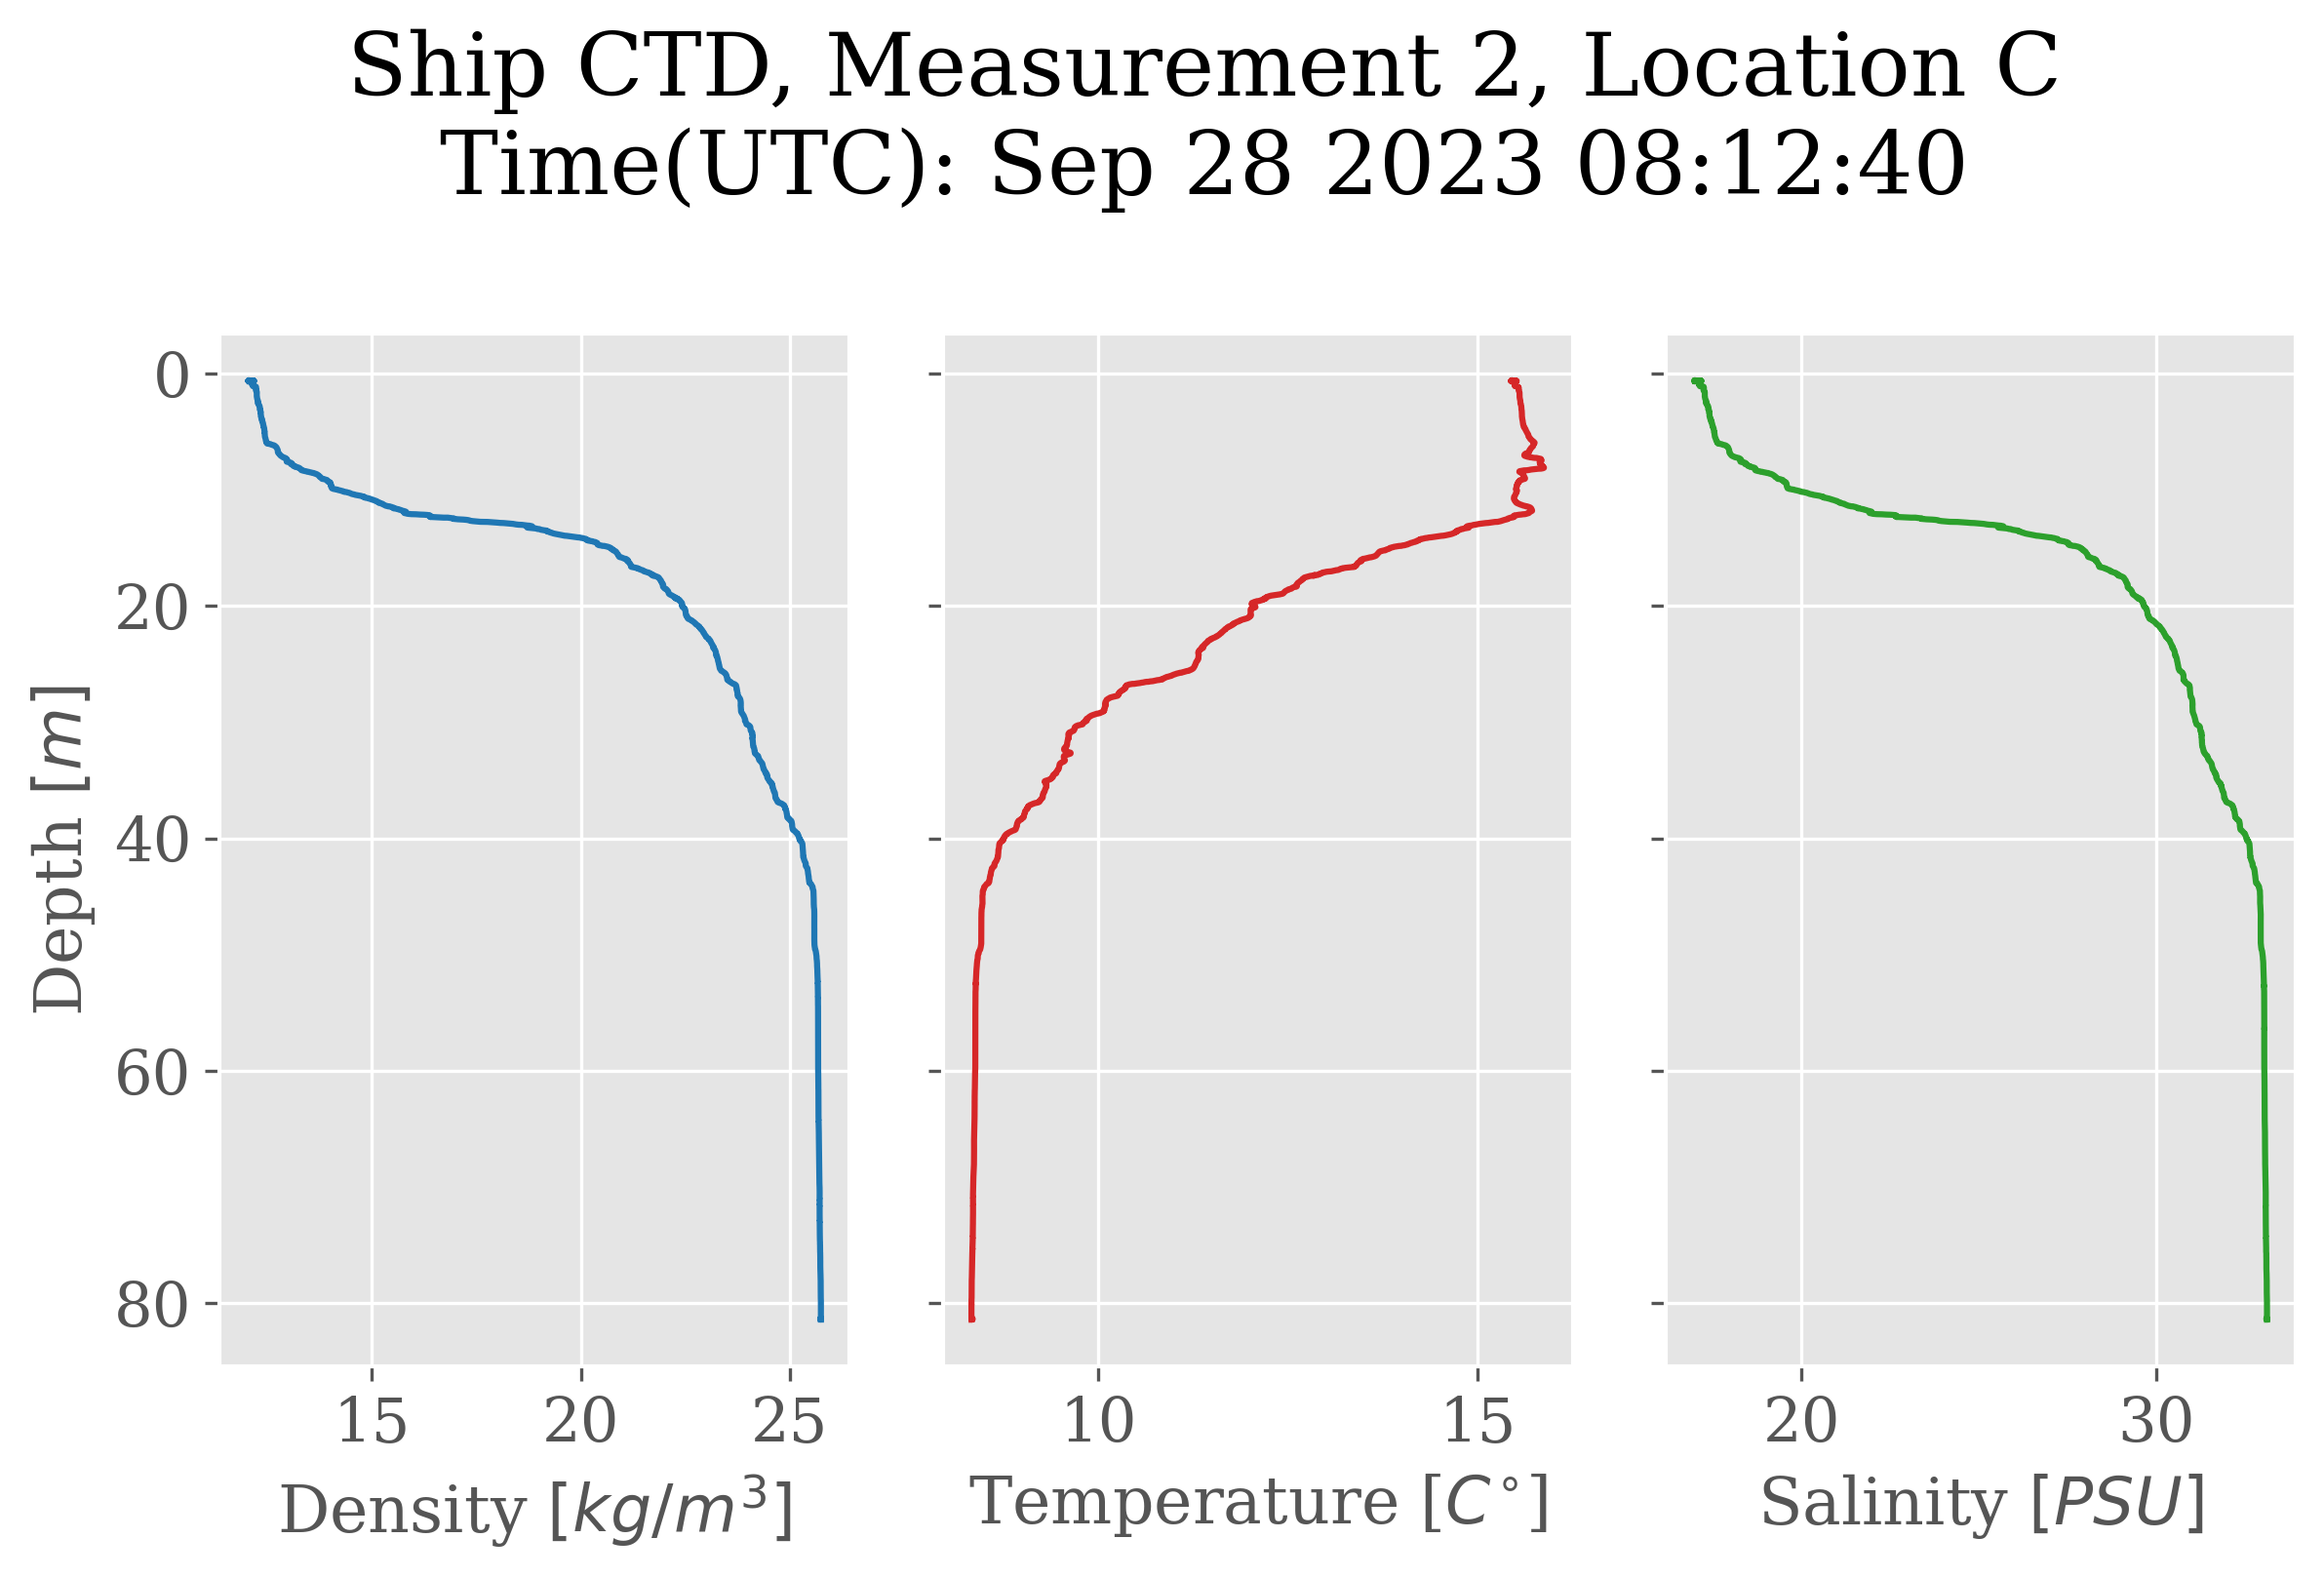
\includegraphics[width=.9\linewidth]{../figures/ship_ctd/ship_ctd_Measurement_2_Location_C.png}
                \caption{}
                \label{fig:ship_m2lC}
            \end{subfigure}%
            \begin{subfigure}{0.65\textwidth}
                \centering
                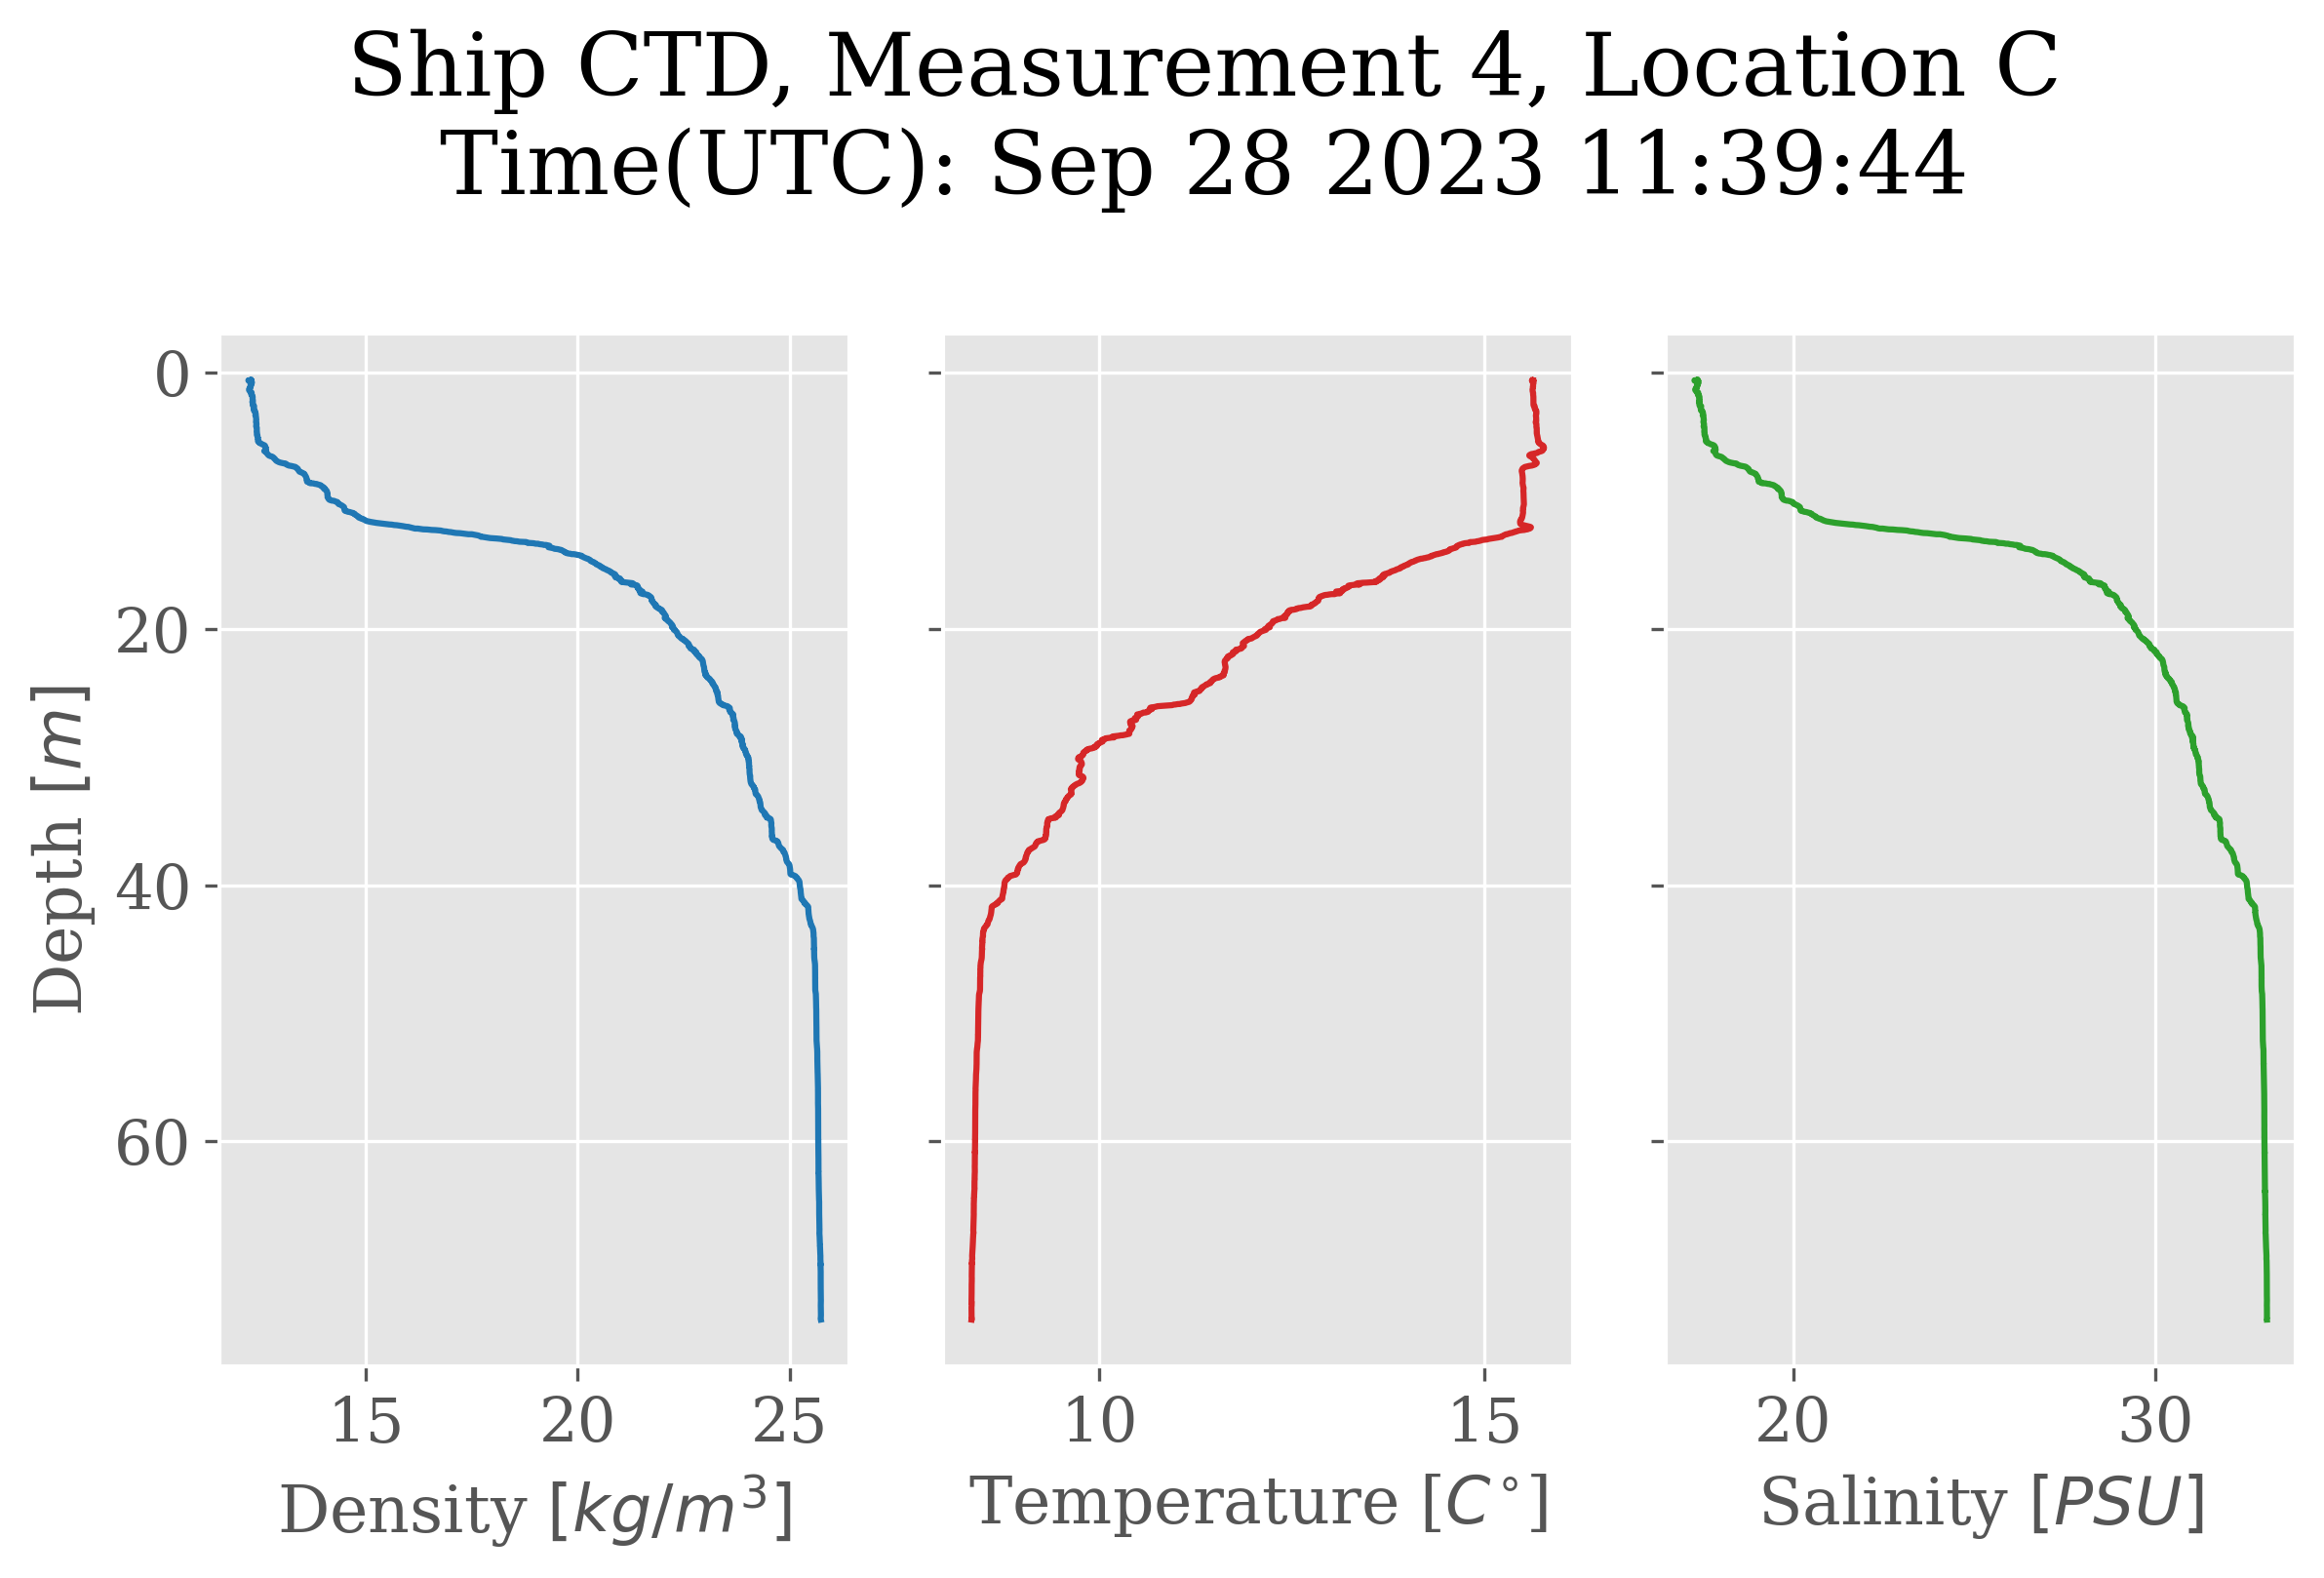
\includegraphics[width=.9\linewidth]{../figures/ship_ctd/ship_ctd_Measurement_4_Location_C.png}
                \caption{}
                \label{fig:ship_m4lC}
            \end{subfigure}
            \end{adjustwidth}
        
            \caption{Handheld (above) and ship (below) CTD measurements at location C. Each shows a depth profile of density, temperature and salinity.}
            \label{fig:location_Capp}
        \end{figure}
    
    
    \subsection{Individual ROMS model profiles with timestamps}\label{app:model}
    % ROMS MODEEL profiles
    \begin{figure}[H]
            \begin{adjustwidth}{-2.5cm}{-2.5cm}  % Adjust the values to change the margins
            \begin{subfigure}{0.65\textwidth}
                \centering
                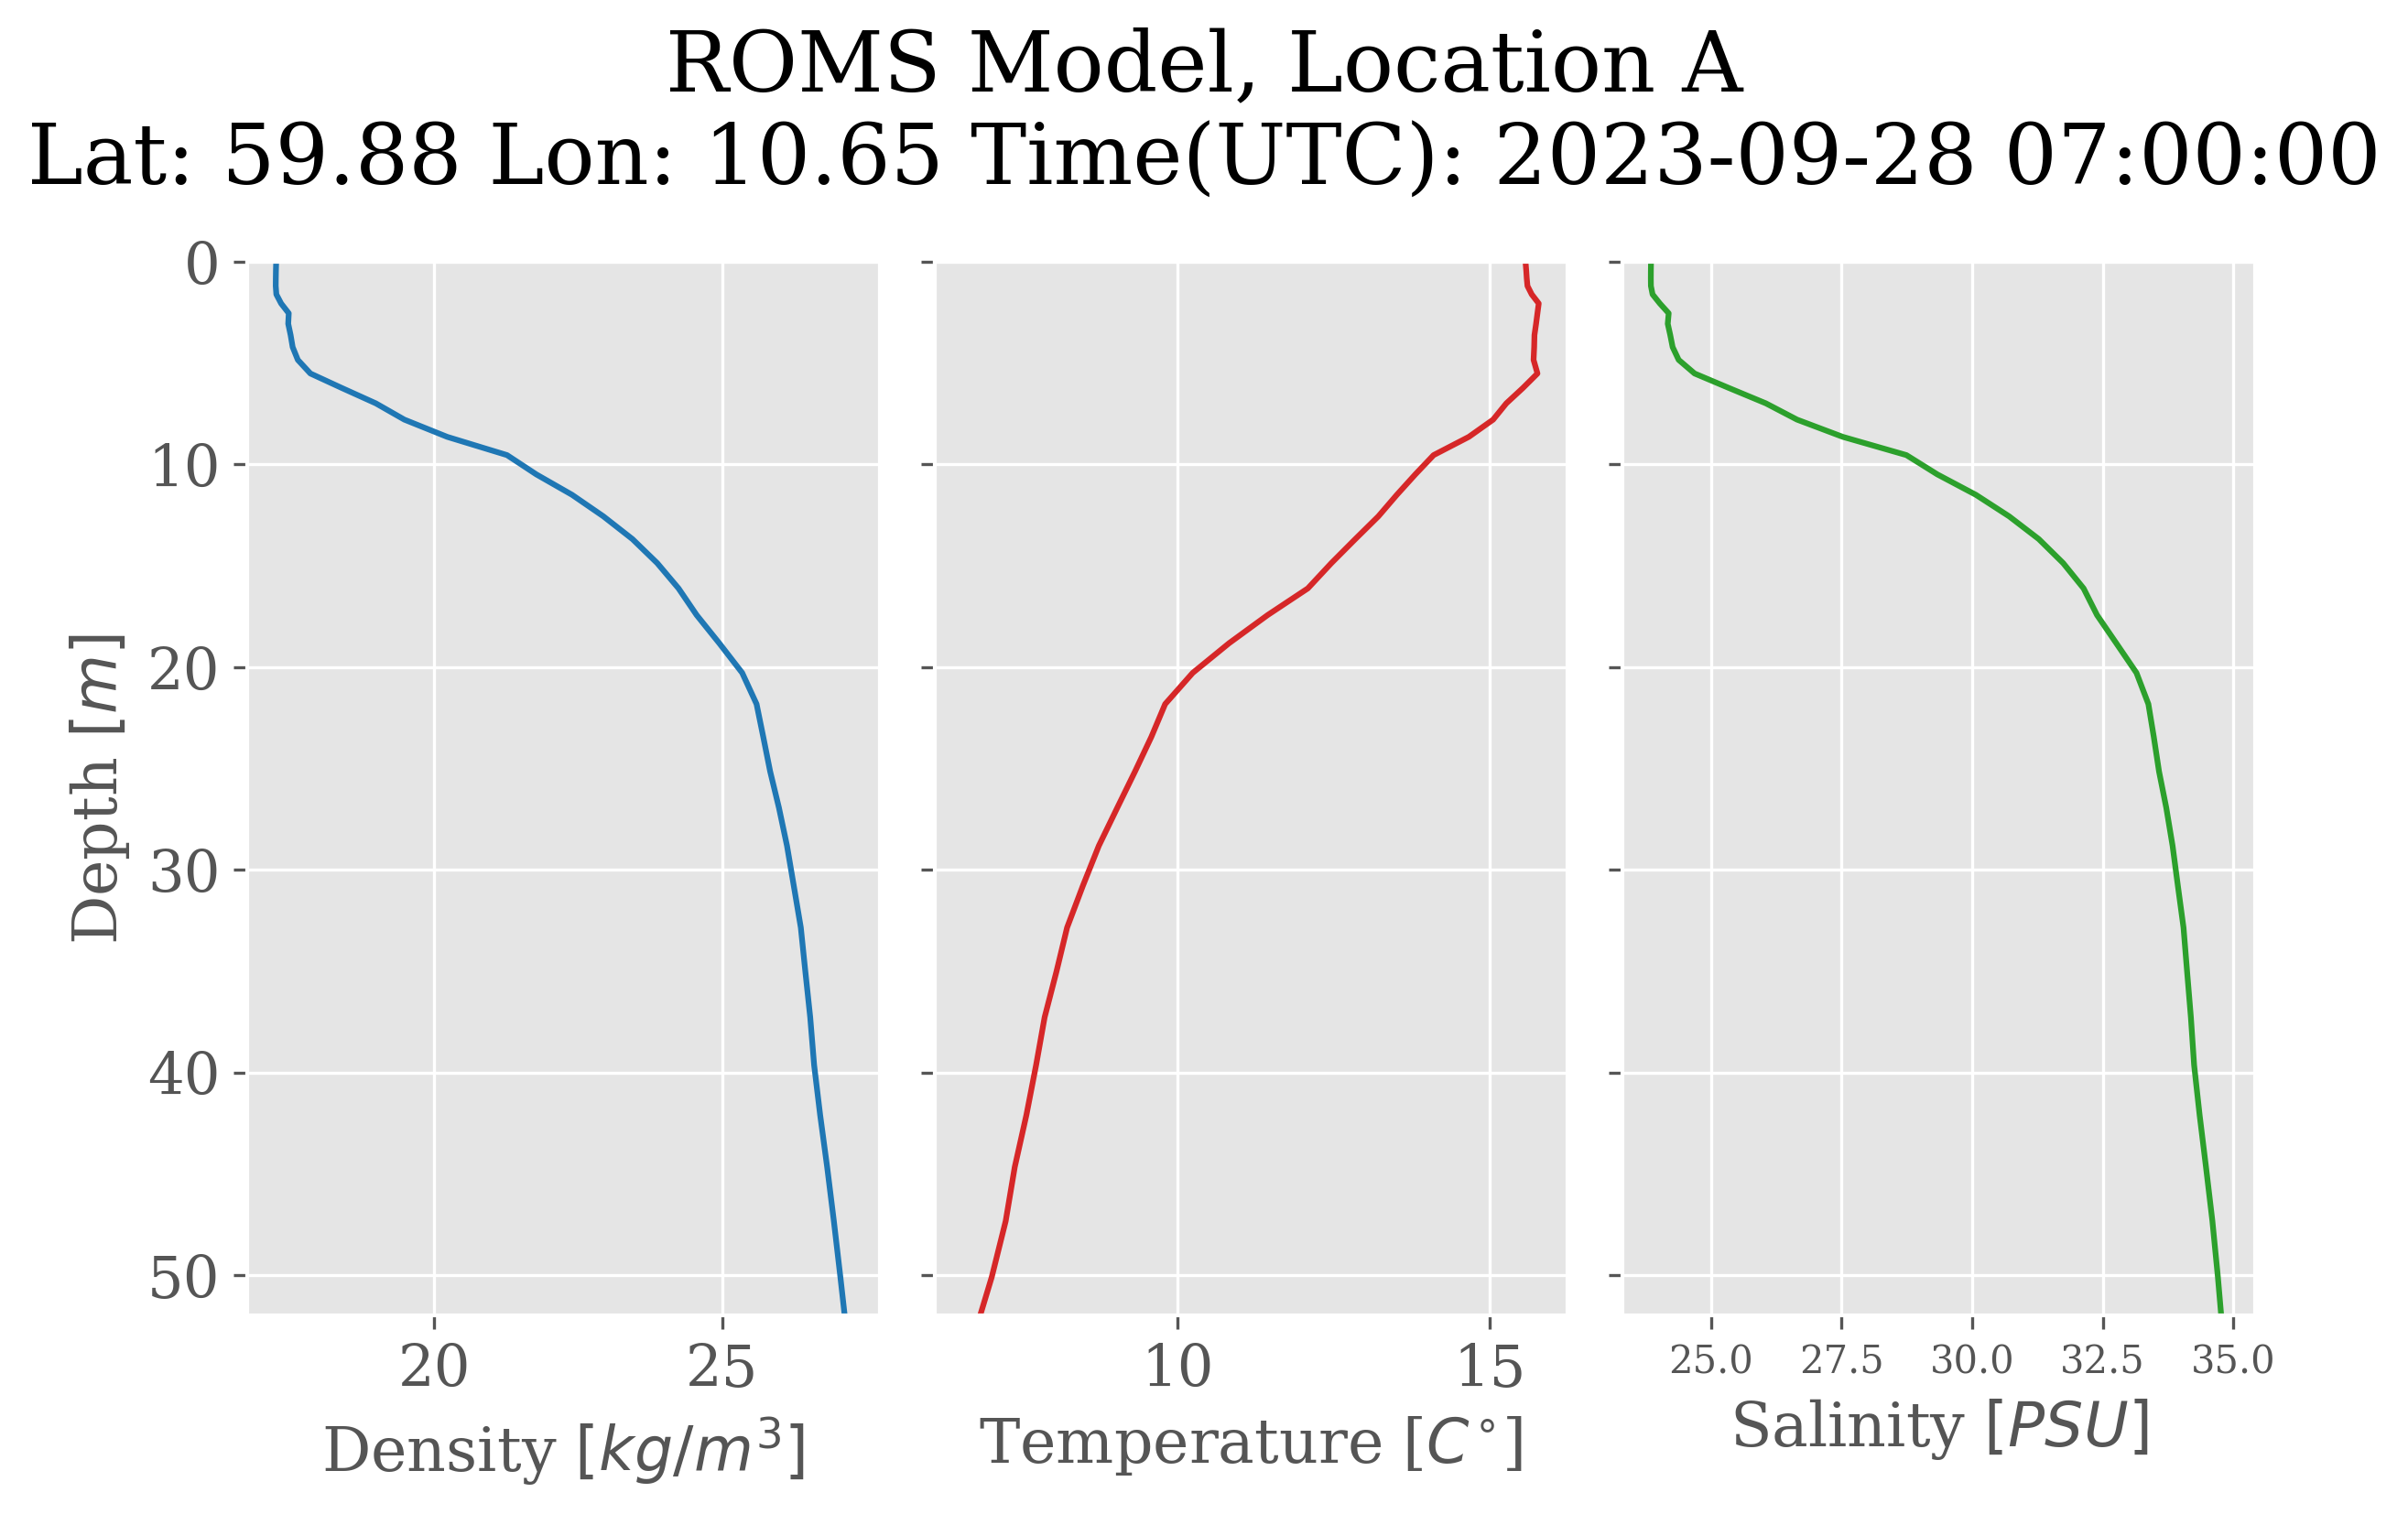
\includegraphics[width=1.\linewidth]{../figures/model_profiles/model_profiles_A_2023_09_28_07.png}
                \caption{}
                \label{fig:model_A07}
            \end{subfigure}%
            \begin{subfigure}{0.65\textwidth}
                \centering
                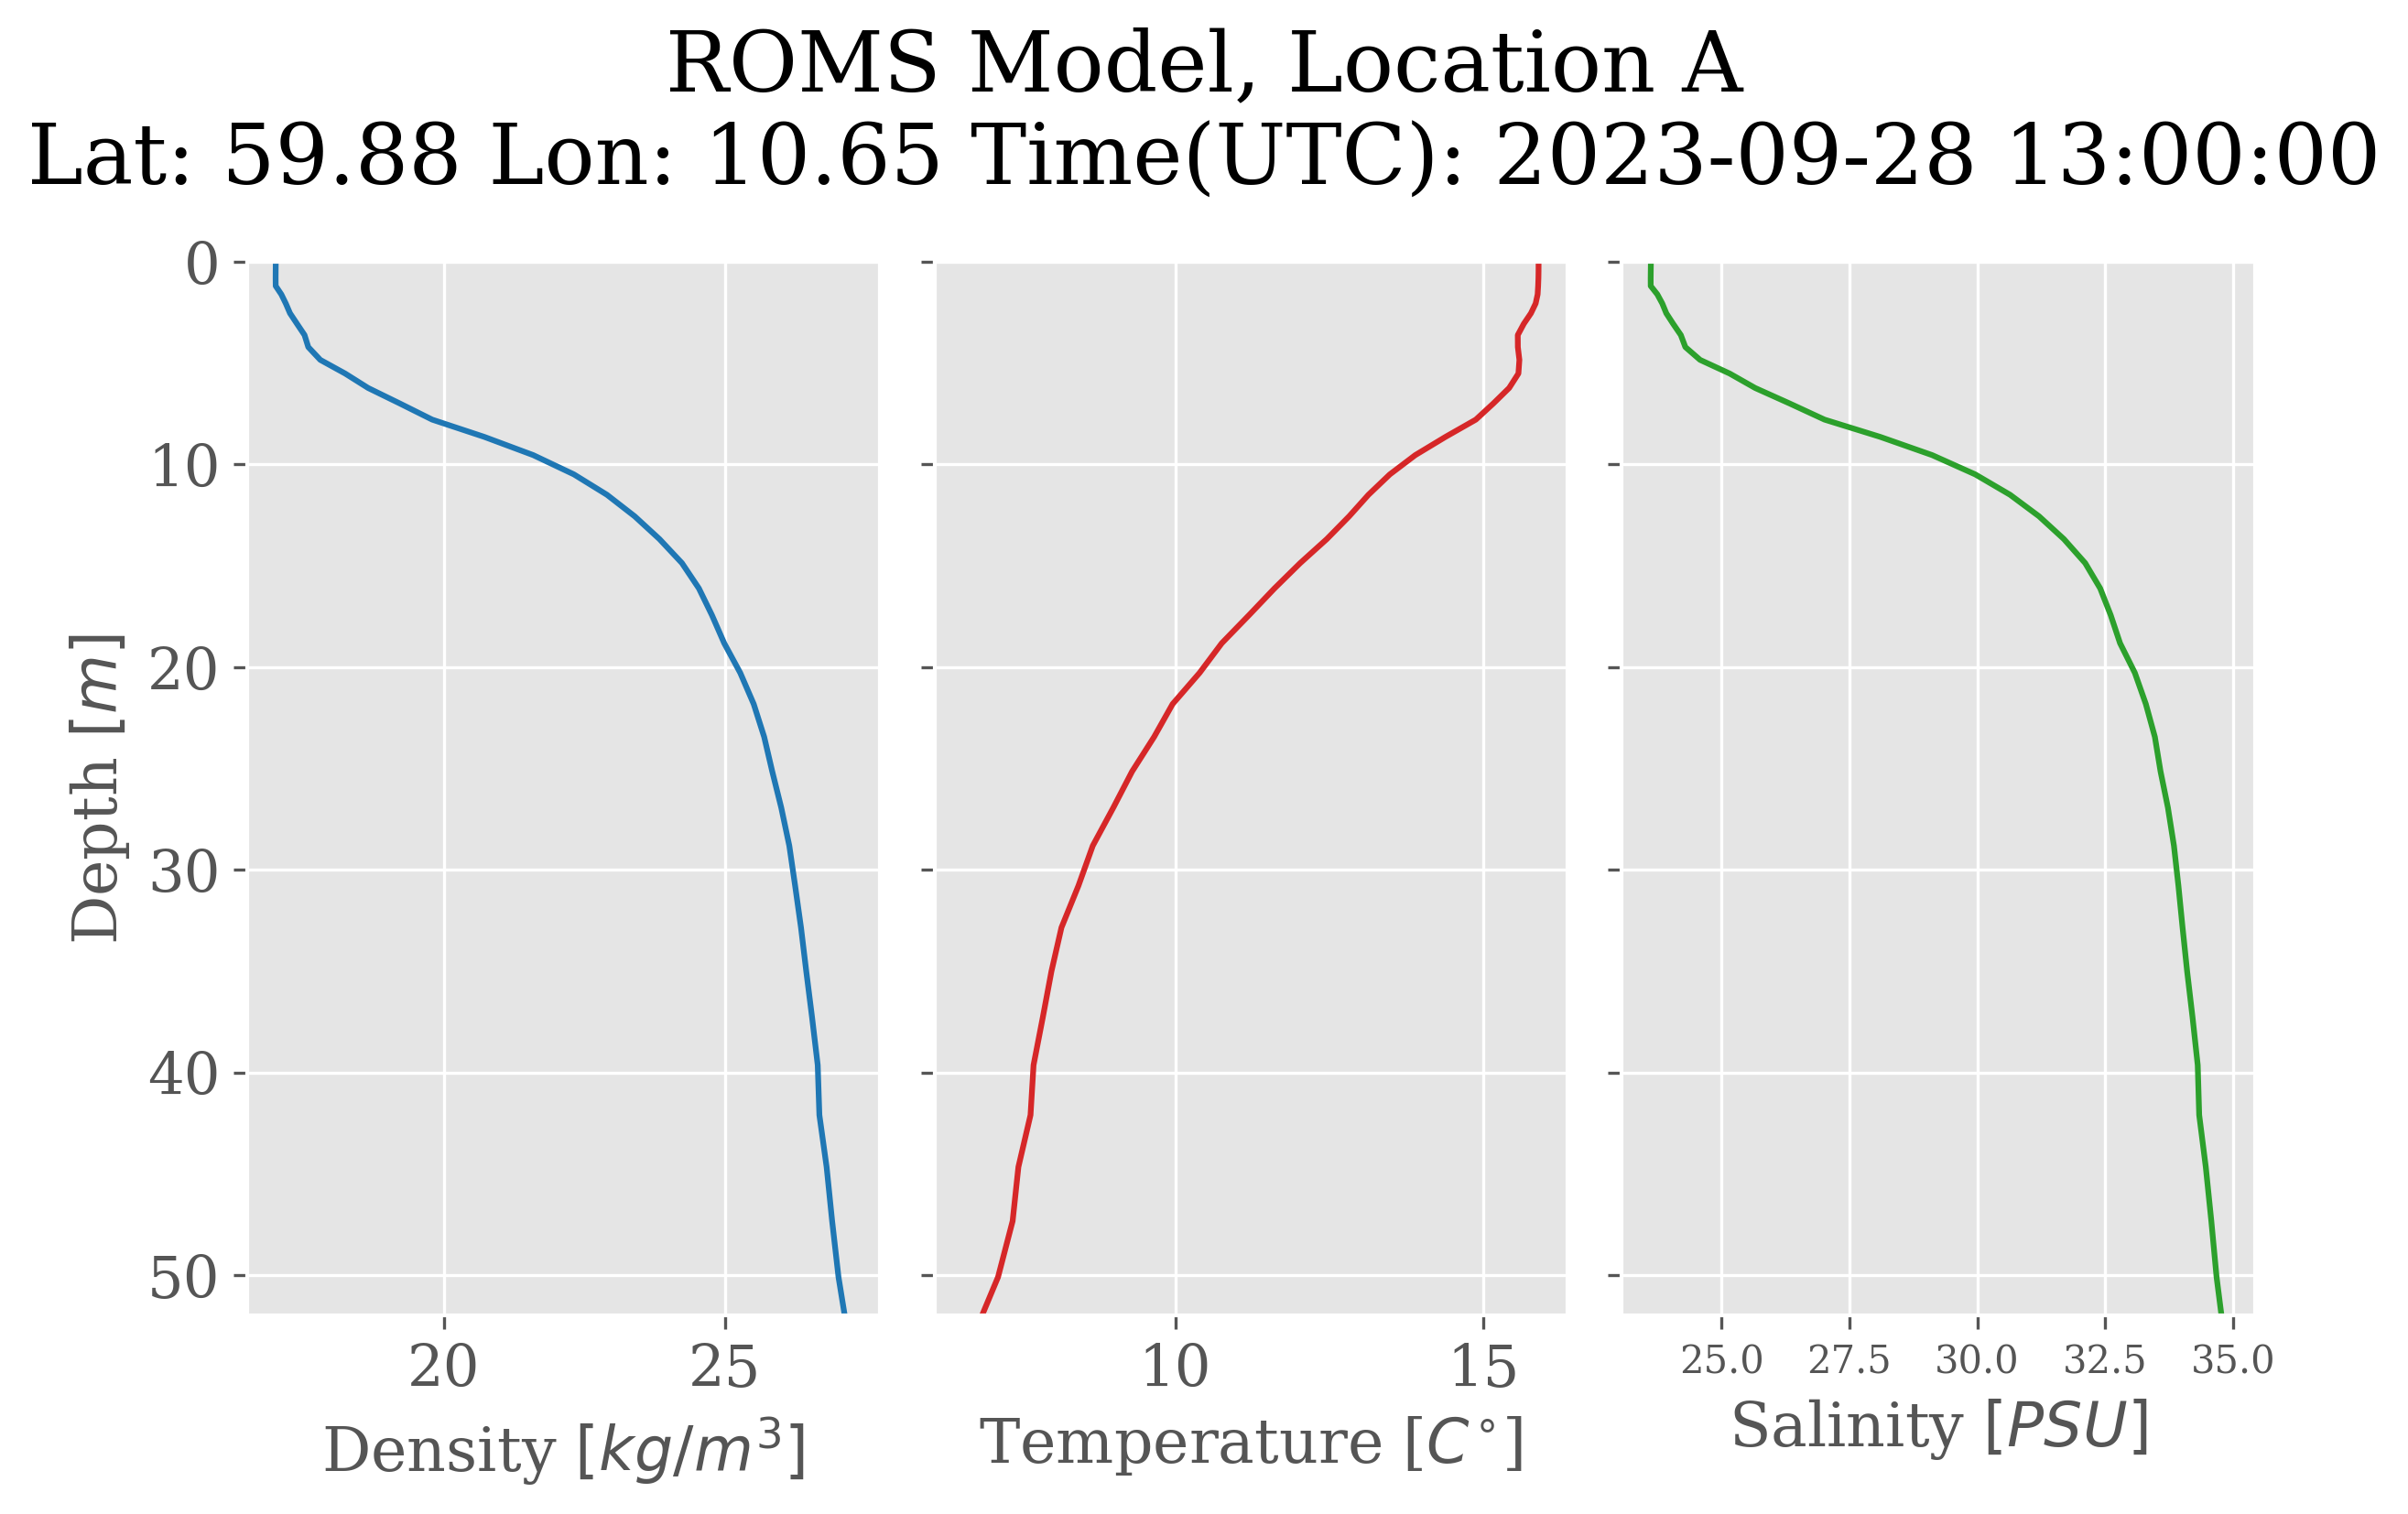
\includegraphics[width=1.\linewidth]{../figures/model_profiles/model_profiles_A_2023_09_28_13.png}
                \caption{}
                \label{fig:model_A13}
            \end{subfigure}
        
            \begin{subfigure}{0.65\textwidth}
                \centering
                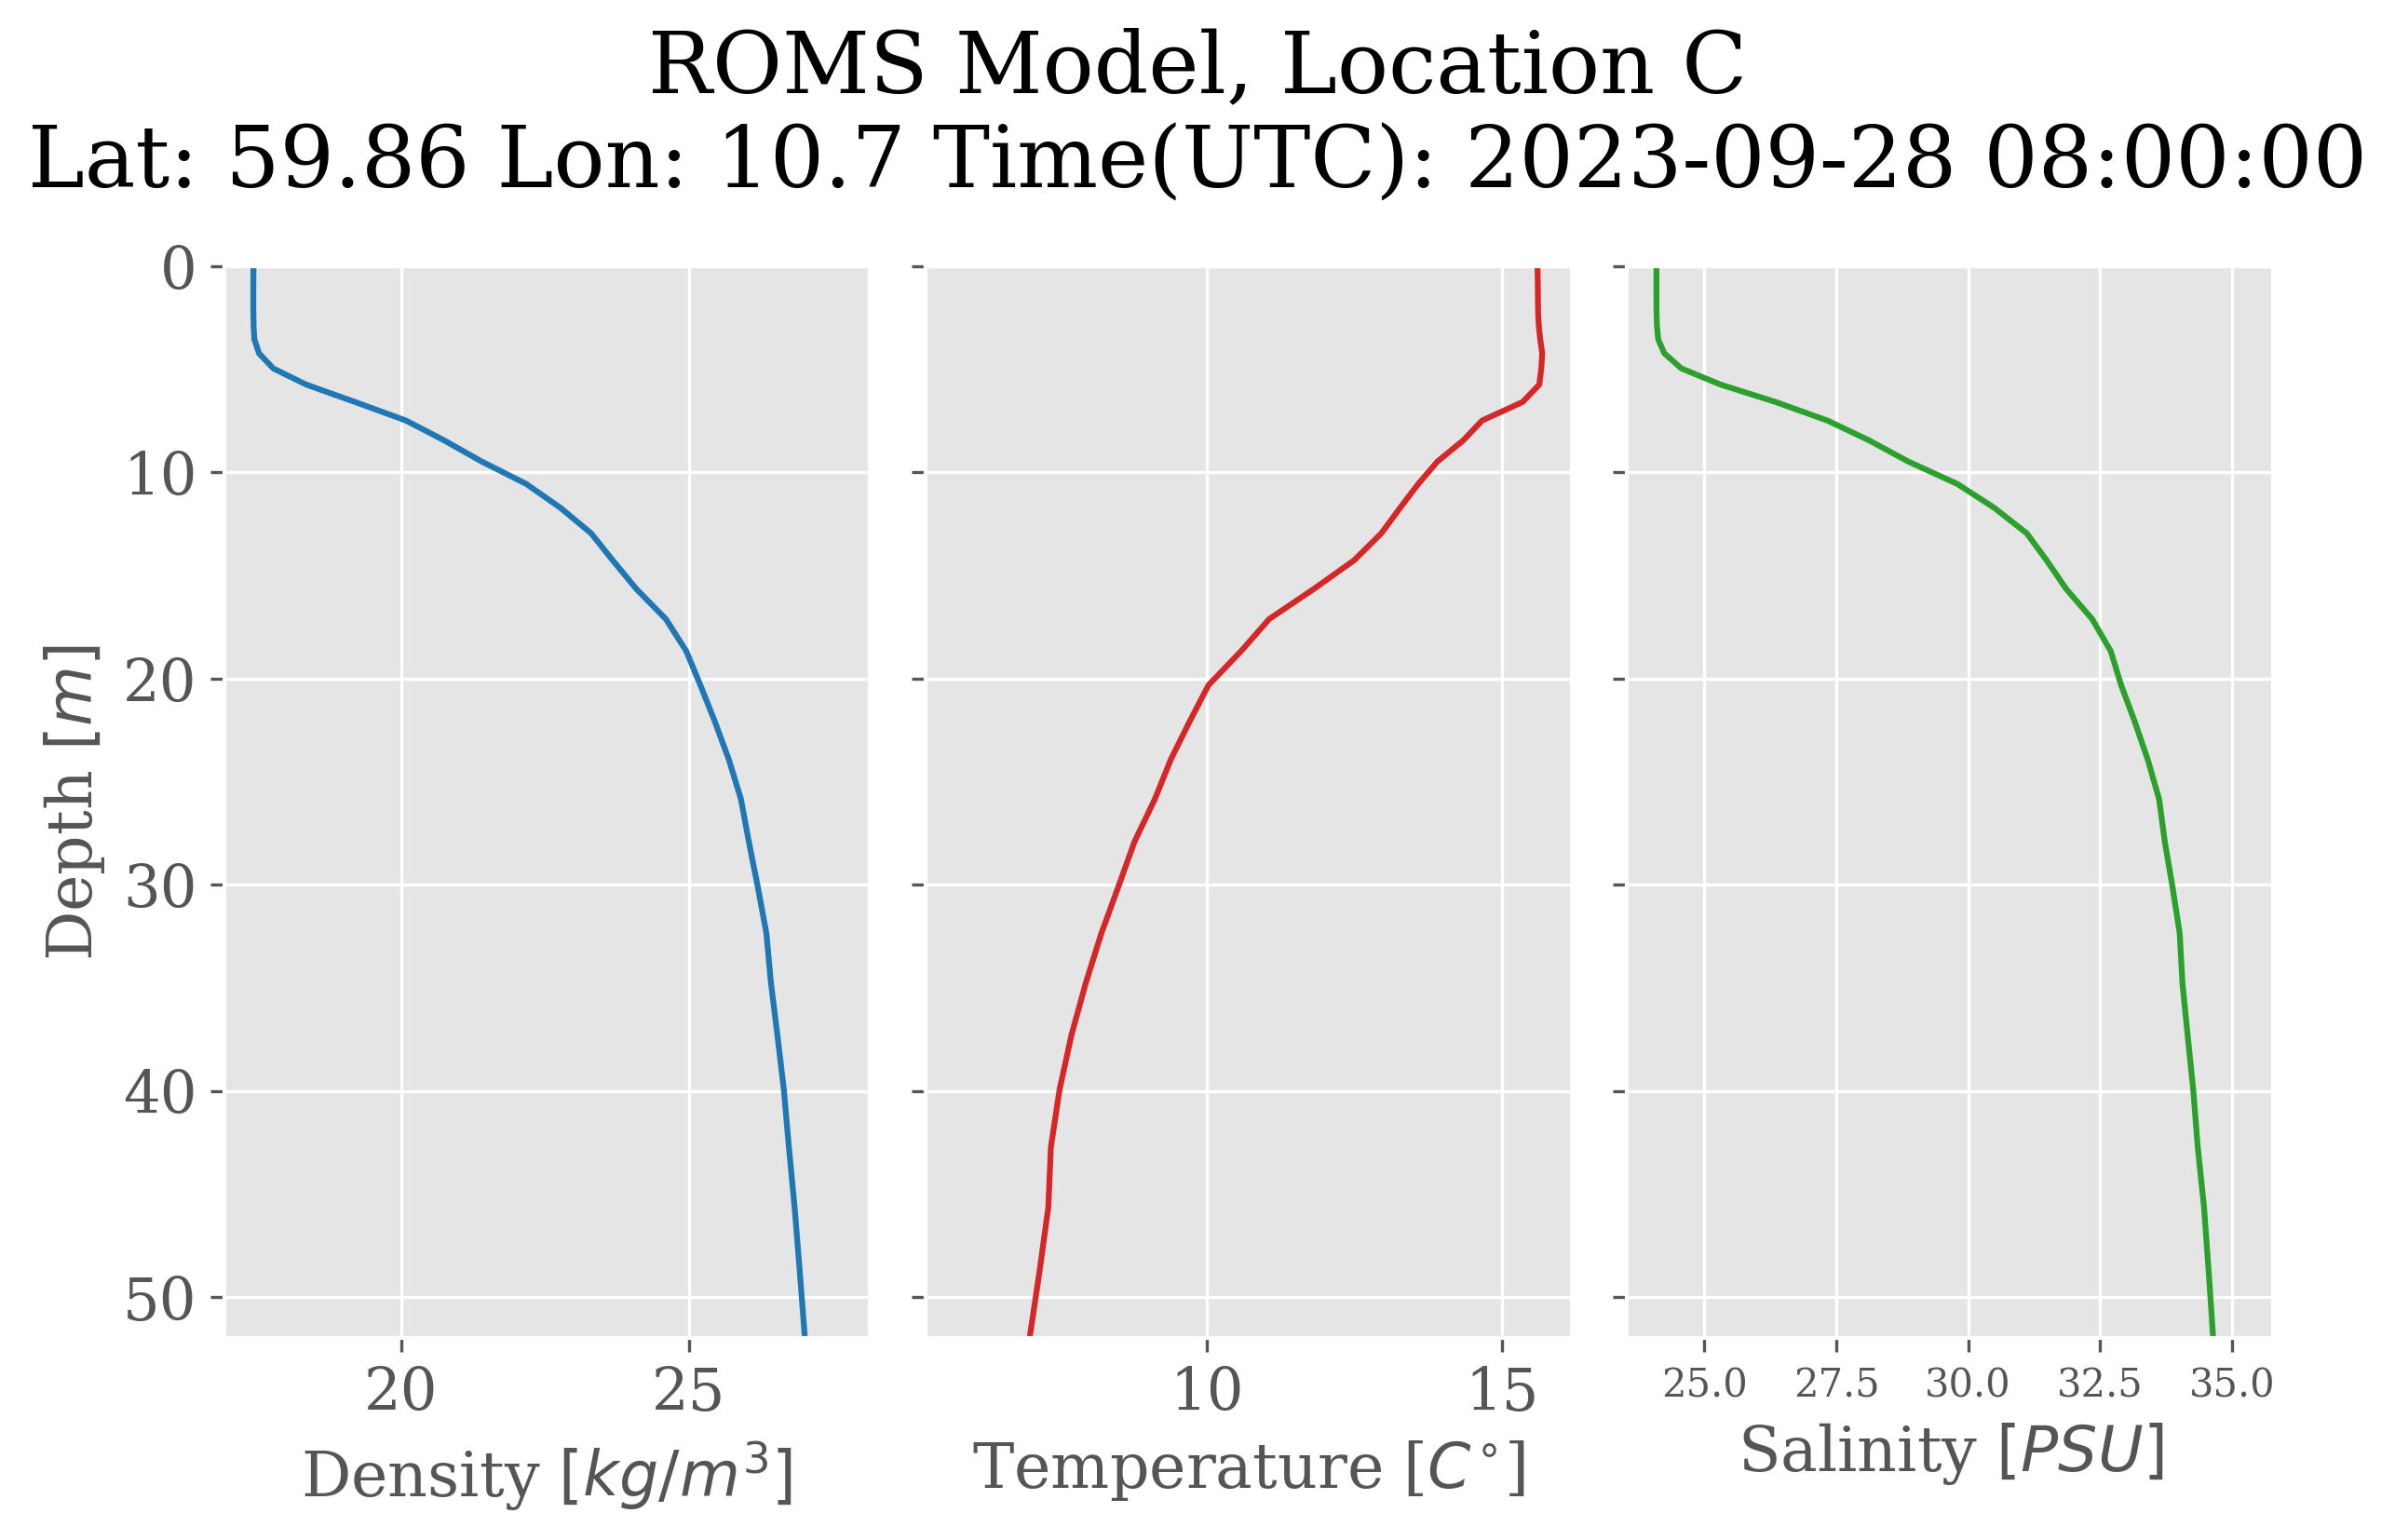
\includegraphics[width=.9\linewidth]{../figures/model_profiles/model_profiles_C_2023_09_28_08.png}
                \caption{}
                \label{fig:model_C08}
            \end{subfigure}%
            \begin{subfigure}{0.65\textwidth}
                \centering
                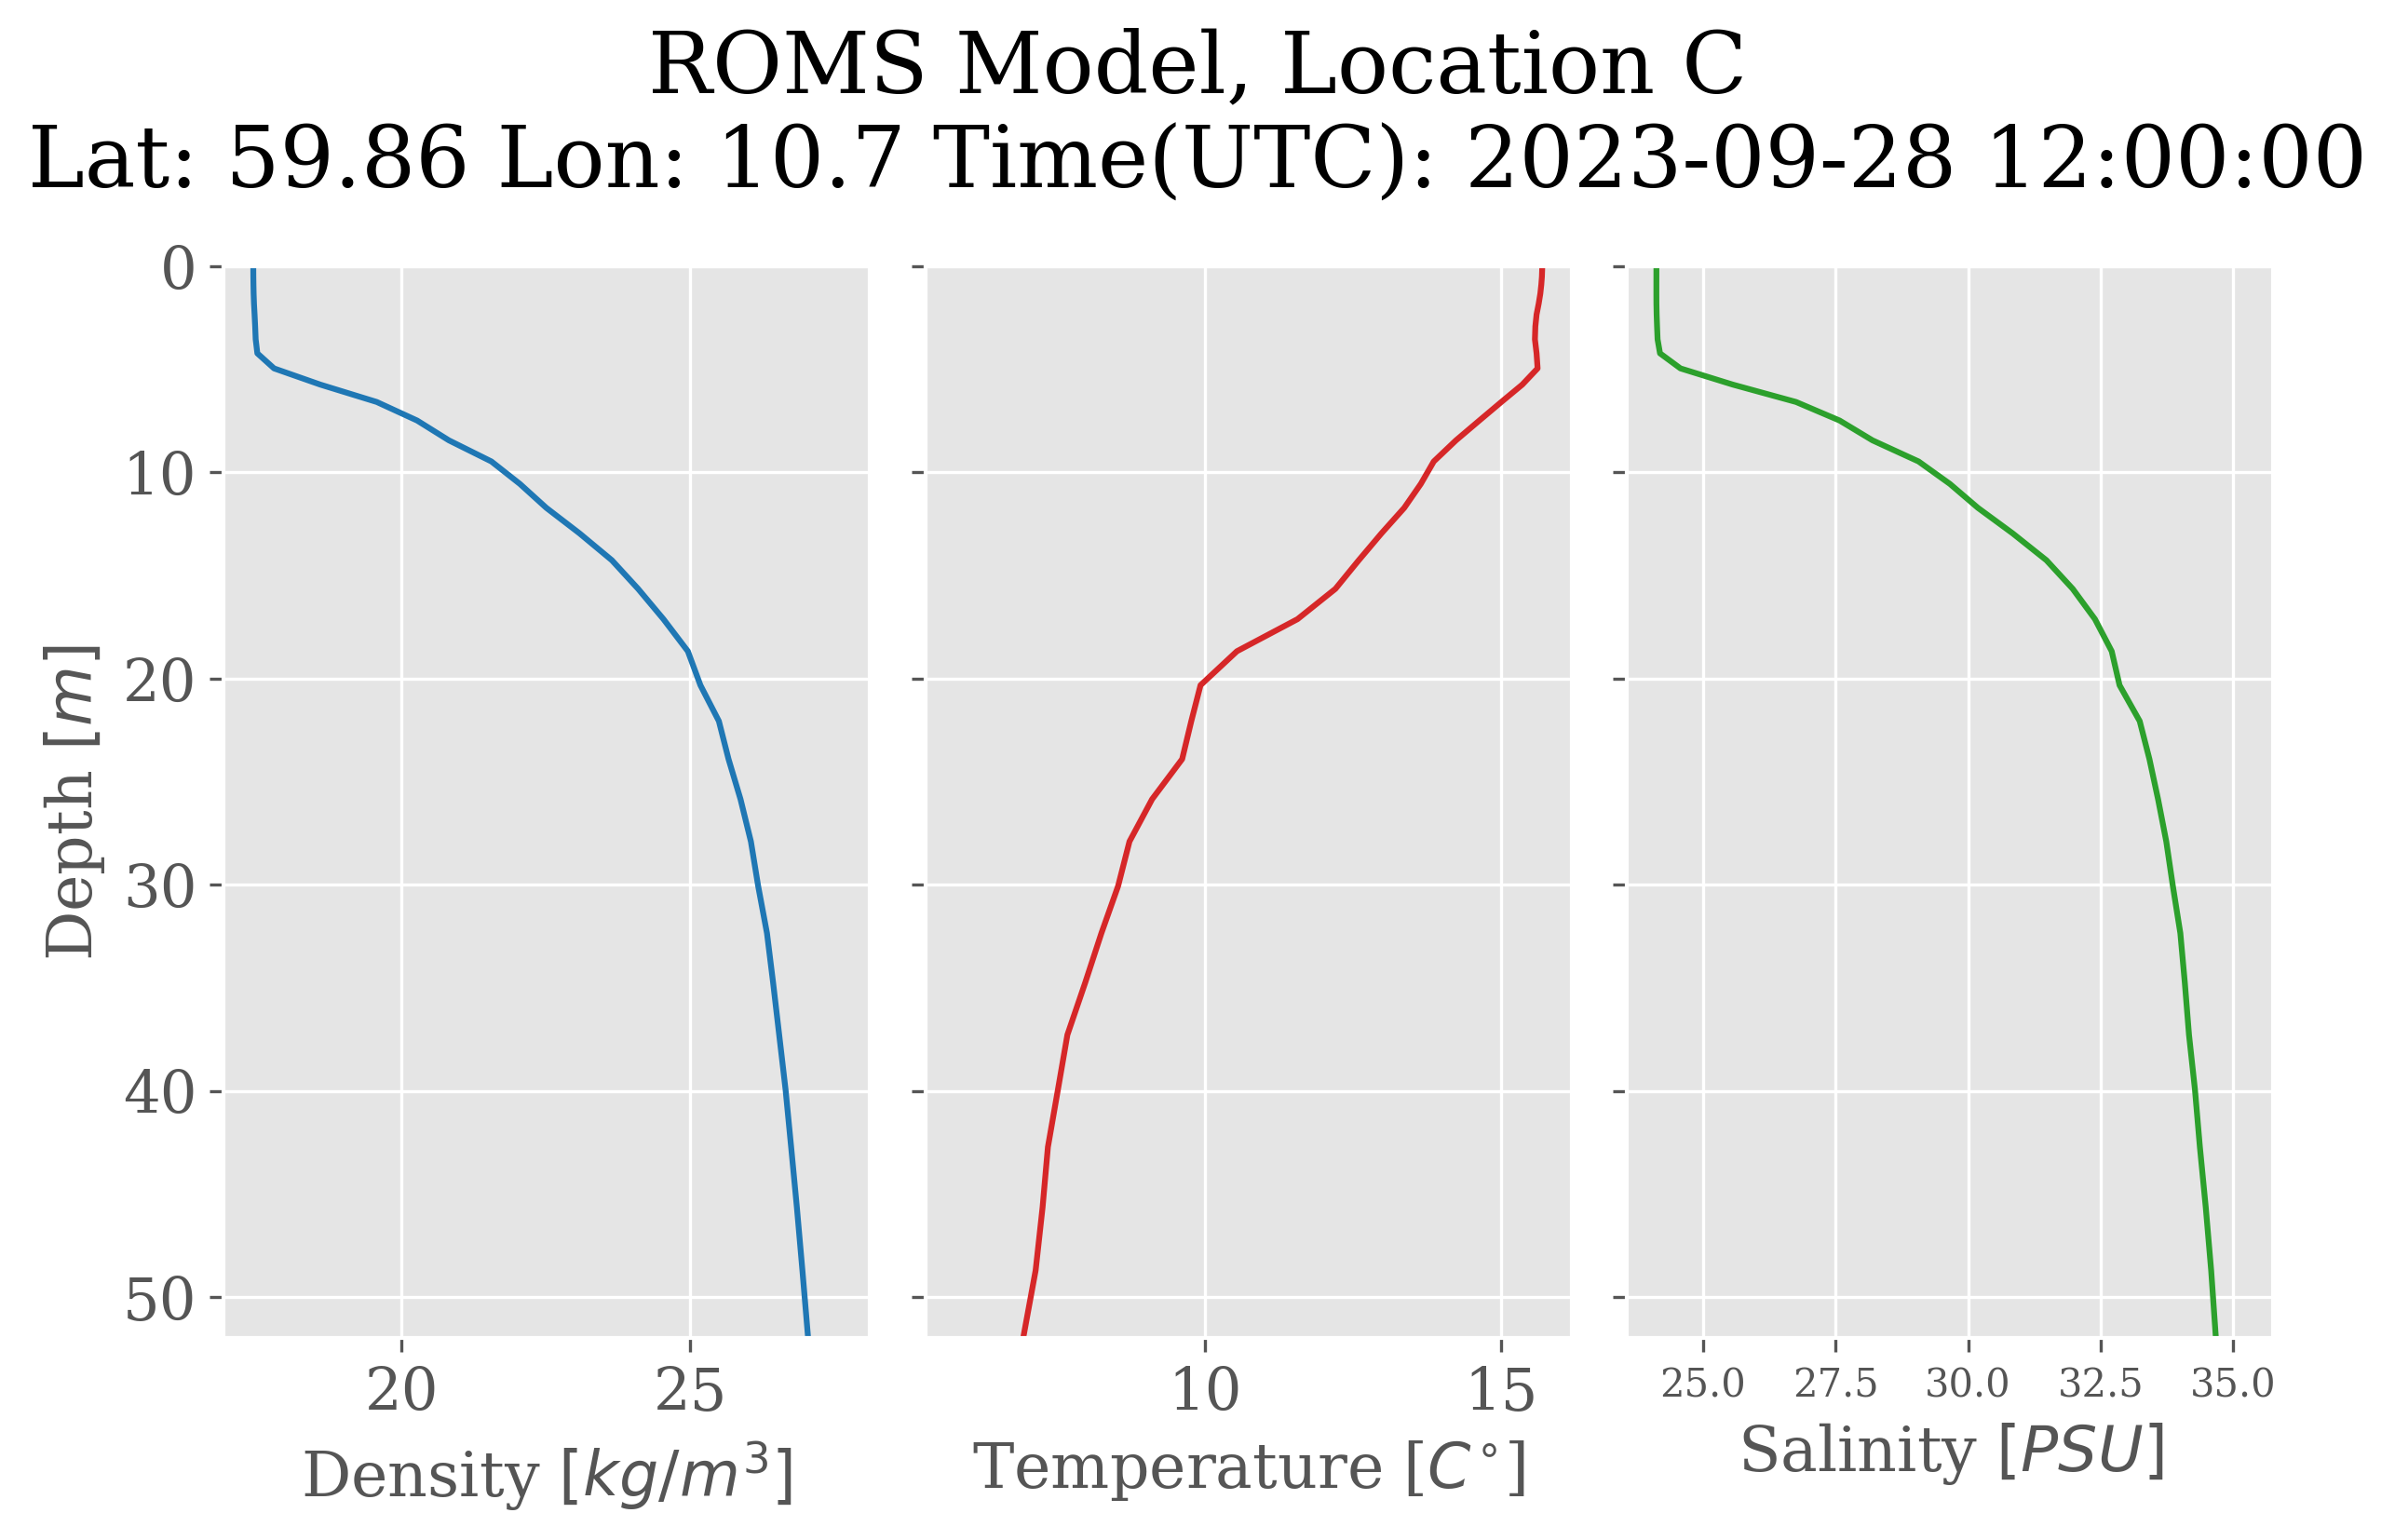
\includegraphics[width=.9\linewidth]{../figures/model_profiles/model_profiles_C_2023_09_28_12.png}
                \caption{}
                \label{fig:model_C12}
            \end{subfigure}
            \end{adjustwidth}
        
            \caption{Profiles at locations A and C generated from the MET Norway ROMS model.}
            \label{fig:model_profiles}
        \end{figure}


\end{document}
